% =====================================================================
%  ME 306 -- sCO2 Brayton cycle project
%  Theory and Implementation
%  Build:  latexmk -pdf theory_and_implementation.tex
% =====================================================================
\documentclass[11pt,a4paper]{report}

\usepackage[margin=2.5cm]{geometry}
\usepackage{amsmath,amssymb}
\usepackage{siunitx}
\usepackage{booktabs}
\usepackage{lmodern}
\usepackage[T1]{fontenc}
\usepackage{microtype}
\usepackage{graphicx}
\usepackage{tikz}
\usepackage{pgfplots}
\usepackage{listings}
\usepackage[most]{tcolorbox}
\usepackage[colorlinks=true,linkcolor=black,citecolor=black,urlcolor=blue]{hyperref}

\pgfplotsset{compat=1.17}
\usetikzlibrary{arrows.meta,positioning,calc,fit,backgrounds}
\sisetup{per-mode=symbol, detect-weight=true}

% ---------------------------------------------------------------- styles
\definecolor{cold}{RGB}{214,230,246}
\definecolor{hot}{RGB}{250,228,215}
\definecolor{neut}{RGB}{238,238,234}
\definecolor{accent}{RGB}{83,74,183}
\definecolor{warn}{RGB}{153,60,29}
\definecolor{chalk}{RGB}{47,102,78}
\definecolor{chalkbg}{RGB}{240,247,243}

\tikzset{
  blk/.style   ={draw=black!55, rounded corners=2pt, align=center,
                 font=\small, minimum height=8mm, minimum width=22mm,
                 inner sep=3pt, line width=0.4pt},
  coldblk/.style={blk, fill=cold},
  hotblk/.style ={blk, fill=hot},
  neutblk/.style={blk, fill=neut},
  ar/.style    ={-{Stealth[length=2mm,width=1.6mm]}, line width=0.5pt},
  lbl/.style   ={font=\scriptsize, inner sep=1.5pt},
}

% caveat box: every one states the choice and what it costs
\newtcolorbox{caveat}[1][]{
  enhanced, breakable, colback=warn!4, colframe=warn!60,
  boxrule=0.4pt, left=3mm, right=3mm, top=2mm, bottom=2mm,
  fonttitle=\bfseries\small, coltitle=warn!80!black,
  title={Caveat},#1}

\newtcolorbox{choicebox}[1][]{
  enhanced, breakable, colback=accent!4, colframe=accent!50,
  boxrule=0.4pt, left=3mm, right=3mm, top=2mm, bottom=2mm,
  fonttitle=\bfseries\small, coltitle=accent!80!black,
  title={Implementation},#1}

\newcommand{\code}[1]{\texttt{\small #1}}

% File paths set in \code are long, unhyphenatable words. Without a little
% slack TeX overfills the line rather than stretching the one before it.
\emergencystretch=3em

% Provenance of a worked number.  Every concrete figure in this document
% is either invented for teaching -- in which case it is round and says
% so -- or computed, in which case this macro names the file it lives in
% and the command that regenerates it.  The point is that you should
% never have to wonder which kind you are reading.
% Two arguments: the saved file, and the command that regenerates it.
% Both are \detokenize'd so that underscores -- which every one of these
% paths contains -- need no escaping at the call site. Escaping file
% paths by hand is exactly the kind of transcription this document is
% trying to get rid of.
\newcommand{\from}[2]{%
  \par\vspace{1pt}\noindent
  {\footnotesize\color{black!55}\textsf{$\hookrightarrow$ computed:
  {\ttfamily\detokenize{results/#1}}\quad regenerate with
  {\ttfamily\detokenize{#2}}}}\par\vspace{4pt}}
\newcommand{\invented}{{\footnotesize\color{black!55}%
  \textsf{(round numbers, invented for the argument)}}}

% Where this document keeps generated tables, plot data and schematics.
% Part II's body is a shared file -- the standalone report compiles the
% same bytes from a different directory and defines these three macros
% to point back here. That is why the body contains no relative paths.
\newcommand{\tbl}[1]{tables/#1}
\newcommand{\dat}[1]{data/#1}
\newcommand{\dgm}[1]{diagrams/#1}

% ------- code excerpts, pulled from source by make_code_snippets.py -------
\lstdefinestyle{pyst}{
  language=Python,
  basicstyle=\ttfamily\scriptsize,
  keywordstyle=\color{chalk!95!black}\bfseries,
  commentstyle=\color{chalk!50!black}\itshape,
  stringstyle=\color{warn!75!black},
  showstringspaces=false,
  breaklines=true, breakatwhitespace=true,
  columns=fullflexible, keepspaces=true,
  tabsize=4, aboveskip=0pt, belowskip=0pt,
}

\newtcbinputlisting{\codefile}[2][]{
  listing only, enhanced, breakable,
  colback=chalkbg, colframe=chalk!55,
  boxrule=0.4pt, left=3mm, right=3mm, top=2mm, bottom=1.5mm,
  fonttitle=\bfseries\scriptsize\ttfamily, coltitle=chalk!85!black,
  attach boxed title to top left={xshift=4mm, yshift=-2.4mm},
  boxed title style={colback=chalkbg, colframe=chalk!55, boxrule=0.4pt,
                     sharp corners, size=small},
  listing file={code/#2}, listing style=pyst, #1}

% ---------------------------------------------------------------- title
\title{\vspace{-1.5cm}\Large\bfseries
  Supercritical \ce{CO2} Brayton Cycle for a Compact SMR\\[2mm]
  \large Theory and Implementation}
\author{\normalsize ME 306 -- Advanced Thermodynamics}
\date{\normalsize Living document. Last rebuilt \today.}

\usepackage[version=4]{mhchem}

\begin{document}
\maketitle

\begin{abstract}
\noindent
This document explains how a supercritical \ce{CO2} power cycle works and
how the solver that models it was built, in that order, because the code
only makes sense once the physics is clear.

It is written to be re-read. Three years from now the code will still be on
the disk and the reasoning behind it will not be in anyone's head, so the
reasoning is here instead: why each approximation was made, what it costs,
and what was tried and abandoned. Worked examples use round invented numbers
chosen so the arithmetic can be followed without a calculator. Every real
computed result is in the appendices, separately, where it can be checked
against a future rebuild without interrupting the explanation.

It is in two parts. Part~I explains the physics and the solver. Part~II
is the submitted report, compiled from the same file the standalone report
uses, so the two can never disagree --- if a conclusion changes, it changes
in one place. Read Part~II first if you want the answer; read Part~I first
if you want to know why it is the answer.

Two companion files sit beside it. \code{usage.md} tells you how to
run the thing, and \code{project\_\allowbreak tracker.md} records what was
decided, when, and why.
\end{abstract}

\tableofcontents

% =====================================================================
\part{Theory and implementation}

This part is the explanation: what the physics is, why the code is shaped
the way it is, and what each approximation costs. Its worked examples use
round invented numbers so the arithmetic can be followed by hand. Part II
is the project's submitted argument, where every figure is a computed one.

\chapter{What this is}

\section{The problem}

A small modular reactor produces \SI{100}{\mega\watt} of heat at around
\SI{500}{\celsius}. Something has to turn that into electricity, and the
question is what.

The obvious answer is a steam cycle, which is what almost every power
station on earth uses. It is well understood and efficient. It is also
enormous: a steam turbine for even a small plant is a multi-stage machine
the size of a bus, the condenser is larger still, and the whole assembly
needs a building put around it. For a reactor whose main selling point is
that it can be built in a factory and trucked to site, the power conversion
system being ten times the size of the reactor is a problem.

Supercritical \ce{CO2} is the alternative being proposed. The claim is that
a \ce{CO2} turbine delivering the same power is roughly the size of a desk,
and that the cycle reaches comparable or better efficiency at the
temperature an SMR can actually provide. The project is to check that claim:
model the cycle properly, compare the layouts that have been proposed for
it, and recommend one.

\section{What has to be decided}

The brief asks for a single recommended configuration, justified on four
grounds that do not agree with each other:

\begin{itemize}\itemsep2pt
\item \textbf{Efficiency.} More electricity from the same reactor.
\item \textbf{Compactness.} Mass and volume, which is the entire reason for
      choosing this cycle.
\item \textbf{Cost.} A proxy, since nobody has real quotes.
\item \textbf{Operational safety.} Behaviour when something is not at its
      design point.
\end{itemize}

The tension is the interesting part. The layouts that reach the highest
efficiency do it by adding heat exchangers, and heat exchangers are the
heaviest, bulkiest and most expensive component in the plant. So efficiency
and compactness pull against each other directly, and a recommendation has
to pick a point on that trade rather than maximise one number.

\section{What was built}

A cycle solver, in two layers.

The lower layer, \code{cycles/}, knows how to solve a flowsheet. It knows
that streams have a pressure, an enthalpy and a flow rate, that blocks
transform streams, and that some property library can answer questions about
whatever fluid it is handed. It does not know what \ce{CO2} is, what a
Brayton cycle is, or what this project is for.

The upper layer, \code{project/}, is this project. It contains the layouts
being compared, the numbers from the brief, and the scripts that produce
results. It uses the lower layer as a black box.

That separation is not decoration. Chapter~\ref{ch:generality} shows what it
bought, which turned out to be more than expected.

\section{How to read this}

It goes physics, then components, then layouts, then how the whole thing is
solved.

Chapters \ref{ch:work} to \ref{ch:props} are physics with no code in them:
why a closed cycle produces work at all, and what supercritical \ce{CO2}
does that breaks the standard formulas.

Chapters \ref{ch:machines} to \ref{ch:precooler} take one component at a
time --- what it does, how it is modelled, then the code --- starting with
the machines, then the recuperator, then everything that rejects heat.

Chapter~\ref{ch:splitting} assembles those components into the four layouts
being compared and argues between them. It comes after the components
rather than before, because the layouts differ in their cooling more than
in anything else and that is not visible until the coolers have been
covered.

Chapter~\ref{ch:solving} is how the pieces are solved together, which is the
hardest part and the most interesting. The rest is shorter. Every real
computed number is a project result and lives in the final report.

Boxes in the margin colour mark two things. A \emph{Caveat} is an
approximation or a limitation, with what it costs. An \emph{Implementation}
box is a design decision that could reasonably have gone another way, with
the reason it went this way. Both are there for the version of you that
comes back later and wonders why.

% =====================================================================
\chapter{Why a closed cycle produces work at all}
\label{ch:work}

\section{The symmetry that has to be broken}

Here is a fact that should be uncomfortable.

The compressor takes the fluid from low pressure to high pressure. The
turbine takes it from high pressure back to low pressure. Same two
pressures, same fluid, same mass flow. One of them consumes work and the
other produces it, and there is no obvious reason the two should not simply
cancel.

For a steady-flow machine with no losses, the work per kilogram is
\begin{equation}
  w = \int v \, \mathrm{d}P
  \label{eq:vdp}
\end{equation}
where $v$ is specific volume. Compression runs the integral one way and
expansion runs it the other, over the same pressure limits. If $v$ were the
same on both passes the two integrals would be equal and opposite, the cycle
would produce exactly nothing, and no amount of clever engineering would
change that.

So the entire question is: \emph{how do you make $v$ different on the way up
and on the way down?}

\section{The answer, and its price}

Make the fluid small when you compress it and large when you expand it.

Specific volume rises with temperature. So compress the fluid cold, when it
takes up little space and the integral is small, then heat it, which
expands it, then expand it hot, when it takes up a lot of space and the
integral is large. The heat added between the two is what buys the asymmetry.

Put round numbers on it. Suppose the pressure span is
\SI{12}{\mega\pascal}, the average specific volume during compression is
\SI{0.002}{\metre\cubed\per\kilogram}, and heating has swollen it to
\SI{0.012}{\metre\cubed\per\kilogram} by the time it reaches the turbine:

\begin{align*}
  w_{\text{compressor}} &\approx 0.002 \times 12 \times 10^6
    = \SI{24}{\kilo\joule\per\kilogram} \\
  w_{\text{turbine}}    &\approx 0.012 \times 12 \times 10^6
    = \SI{144}{\kilo\joule\per\kilogram} \\
  w_{\text{net}}        &= \SI{120}{\kilo\joule\per\kilogram}
\end{align*}

Six times the volume, six times the work out, and the difference is the
plant's entire output.

\section{Back-work ratio, and why it decides everything}
\label{sec:bwr}

The ratio of those two numbers has a name:
\[
  \mathrm{BWR} = \frac{w_{\text{compressor}}}{w_{\text{turbine}}}
  = \frac{24}{144} = 0.17.
\]
Seventeen percent of what the turbine makes goes straight back into the
compressor. The other \SI{83}{\percent} is yours.

This single number separates the major power cycles more cleanly than any
other:

\begin{center}
\begin{tabular}{@{}llp{0.40\linewidth}@{}}
\toprule
Cycle & BWR & Why \\
\midrule
Steam Rankine & $\approx 0.01$
  & The pump handles liquid water, which is almost incompressible.
    $v$ is tiny, so the integral is negligible. \\
Gas turbine & $\approx 0.5$
  & The compressor handles air, a thin gas with large $v$.
    Half the turbine output is eaten. \\
sCO$_2$ & $\approx 0.2$
  & Compression happens where \ce{CO2} is nearly as dense as a liquid. \\
\bottomrule
\end{tabular}
\end{center}

Steam wins this comparison outright, which is why steam cycles exist. The
price is a phase change: you need a boiler and a condenser, and the
condenser is the single largest object in the plant. A gas turbine has no
phase change and is compact, but gives back half its output at the
compressor.

The sCO$_2$ cycle is an attempt to take the good half of each. Compress a
fluid dense enough that the pump argument almost works, but keep it as a
single phase throughout so there is no condenser.

\section{Why \ce{CO2}, and why right there}

For the fluid to be nearly incompressible at the compressor inlet without
being a liquid, it has to sit just above its critical point: dense like a
liquid, continuous like a gas.

\ce{CO2}'s critical point is at \SI{30.98}{\celsius} and
\SI{7.3773}{\mega\pascal}, and both halves of that are a gift. The
temperature is close to what ordinary cooling water can reach, so the
compressor inlet can be held there without refrigeration. The pressure is
high but not unreasonable. For almost any other candidate fluid one or both
numbers are wrong: water's critical point is at \SI{374}{\celsius}, far too
hot to compress at; nitrogen's is at \SI{-147}{\celsius}, requiring
cryogenics.

So the cycle is designed around the compressor inlet sitting a whisker above
that point, at roughly \SI{32}{\celsius} and \SI{7.7}{\mega\pascal}. One
degree and a third of a megapascal clear of critical.

How dense is it there? About a fifth of the volume an ideal gas would occupy
at the same pressure and temperature. The compressibility factor $Z = Pv/RT$
is around \num{0.22}, where an ideal gas would give exactly \num{1}. The
fluid is five times denser than the ideal-gas law predicts, and
Equation~\eqref{eq:vdp} takes that straight off the compressor bill.

\subsection{A sanity check you can do in your head}

There is a quick test of whether a fluid is behaving liquid-like. If $v$
barely changes during compression, it can be pulled out of
Equation~\eqref{eq:vdp} as a constant, giving the pump formula:
\[
  w \approx v_{\text{in}}\, \Delta P.
\]

Apply that to sCO$_2$ at the compressor inlet and it lands within a fraction
of a percent of what the solver computes from real properties. Apply it to
air at ambient conditions and it overestimates by nearly a factor of three,
because air expands enormously while being compressed and $v_{\text{in}}$ is
nothing like the average.

The pump formula working is the test. It means \ce{CO2} at the compressor
inlet is, for the purposes of the work integral, behaving like a liquid.

\begin{caveat}[title={Caveat: this operating point is a knife edge}]
Everything above depends on sitting just above the critical point, and
properties change violently there. A compressor inlet that drifts a couple
of degrees colder can start condensing, and liquid in a compressor is
cavitation, which destroys machinery.

Worse, density near the critical point is extremely sensitive to small
changes in temperature and pressure, so the machine's own operating map
moves under it. This is real and it is one of the open engineering problems
with sCO$_2$ cycles, not a modelling detail. The solver computes design
points and says nothing about this, so any operational-safety claim made
from its output is a claim about the design point only.
\end{caveat}

\section{What to remember}

\begin{itemize}\itemsep2pt
\item Work is $\int v\,\mathrm{d}P$, and compression and expansion run that
      integral in opposite directions over the same pressure span.
\item The cycle produces net work only because heating makes $v$ larger on
      the expansion pass. The heat buys the asymmetry.
\item Back-work ratio is the compressor's share of the turbine's output:
      $\approx 0.01$ for steam, $\approx 0.5$ for a gas turbine,
      $\approx 0.2$ for sCO$_2$.
\item \ce{CO2} is chosen because its critical temperature is near ambient,
      so the compressor can sit just above it where the fluid is dense.
\item That operating point is narrow, and the narrowness is a real
      operational risk rather than a modelling inconvenience.
\end{itemize}

% =====================================================================
\chapter{What the fluid is actually doing}
\label{ch:props}

\section{Above the critical point, where the rules change}

Below the critical point a fluid has two states and a sharp line between
them. Heat a liquid at constant pressure and its temperature climbs until it
reaches the boiling point, where it stops dead: all the heat you add goes
into converting liquid to vapour at constant temperature, and only once the
last drop has boiled does the temperature start rising again. The flat part
is the latent heat.

Raise the pressure and that flat part gets shorter, because liquid and
vapour become more alike. At the critical point it vanishes entirely. Above
it there is no boiling, no latent heat, no distinction between liquid and
vapour, and no line to cross. The fluid is simply one continuous phase whose
density you can vary from gas-like to liquid-like by changing pressure and
temperature.

That is the useful part: it is why the compressor can work on something
nearly as dense as a liquid without any risk of the two-phase mess that
would wreck it.

\section{The line that does not quite disappear}

The phase boundary vanishes, but it leaves something behind.

Follow the saturation line up to the critical point and continue past it in
the same direction. Along that extension the fluid still does something
reminiscent of boiling: over a narrow temperature band it absorbs a great
deal of heat while barely warming. There is no phase change and no latent
heat, but the specific heat $c_p$ goes through a sharp peak, as if the
fluid remembers how to boil and is doing a smeared-out version of it.

That extension is the \textbf{pseudo-critical line}, and the peak is the
single most important feature of this entire cycle.

\begin{figure}[htbp]
\centering
\begin{tikzpicture}
\begin{axis}[width=12cm, height=5.6cm,
  xlabel={Temperature [\si{\celsius}]},
  ylabel={$c_p$ [\si{\kilo\joule\per\kilogram\per\kelvin}]},
  xmin=25, xmax=150, ymin=0, ymax=16,
  legend pos=north east, legend style={font=\small,draw=black!30},
  grid=both, grid style={black!8},
  tick label style={font=\small}, label style={font=\small}]
\addplot[accent, thick] table[x=T,y=cp_lp] {data/cp_co2.dat};
\addlegendentry{\SI{7.7}{\mega\pascal}, low-pressure side}
\addplot[warn, thick] table[x=T,y=cp_hp] {data/cp_co2.dat};
\addlegendentry{\SI{20}{\mega\pascal}, high-pressure side}
\end{axis}
\end{tikzpicture}
\caption{Specific heat of \ce{CO2} near the compressor inlet. At
\SI{7.7}{\mega\pascal}, barely above critical, the peak is tall and narrow.
At \SI{20}{\mega\pascal} it has flattened into a broad hump. The two sides
of the recuperator run at these two pressures, which is why they behave
differently in the same exchanger.}
\label{fig:cp}
\end{figure}

Two things in that figure matter later.

\textbf{The peak is tall.} Near it, a \SI{10}{\kelvin} temperature rise can
cost around \SI{150}{\kilo\joule\per\kilogram} of enthalpy. Out at
\SI{400}{\celsius}, where $c_p$ has settled near
\SI{1.2}{\kilo\joule\per\kilogram\per\kelvin}, the same
\SI{10}{\kelvin} costs \SI{12}{}. The same temperature change costs
\emph{twelve times} as much enthalpy depending on where you are.

\textbf{The peak moves and flattens with pressure.} The two curves in
Figure~\ref{fig:cp} are the same fluid at the two pressures the recuperator
operates between, and they are not the same shape. Chapter~\ref{ch:splitting}
is entirely about the consequences of that mismatch.

\section{Why the formula sheet stops working}

The standard Brayton analysis is three equations, and the \ce{CO2} cycle
breaks all three.

\begin{center}
\begin{tabular}{@{}llp{0.42\linewidth}@{}}
\toprule
Assumption & What it says & Why it fails here \\
\midrule
Ideal gas & $Pv = RT$
  & $Z \approx 0.22$ at the compressor inlet. Off by a factor of five. \\
Constant $c_p$ & $\Delta h = c_p \Delta T$
  & $c_p$ runs from about \SI{1.2}{} to \SI{15}{\kilo\joule\per\kilogram
    \per\kelvin} within one cycle. \\
Isentropic relation & $T_2/T_1 = (P_2/P_1)^{(\gamma-1)/\gamma}$
  & Derived from the first two, so it inherits both failures. \\
\bottomrule
\end{tabular}
\end{center}

This is not a matter of accuracy. These relations do not give a slightly
wrong answer near the critical point; they give a meaningless one. Every
closed-form result on a Brayton formula sheet has to be abandoned, and the
properties have to come from a real equation of state.

\section{What replaces them}

Modern property libraries do not store tables. They store a single
function, the Helmholtz free energy $a(T, \rho)$, fitted to experimental
data, from which every other property follows by differentiation. Pressure
is a first derivative, entropy another, specific heat a second derivative,
and so on. One fitted function, consistent properties everywhere, including
through the critical region where simpler models fall apart.

\begin{choicebox}
\textbf{CoolProp} is used here, through a thin adapter in
\code{cycles/properties/}. Wrapping it rather than calling it directly costs
one layer of indirection and buys three things: the solver can be handed a
different backend (an ideal gas, for the validation in
Appendix~\ref{app:validation}), the property calls are in one place if they
ever need caching, and no block ever imports CoolProp, so no block depends
on it.
\end{choicebox}

\section{Which two properties to carry}

A state needs two independent properties. Which two is a real decision, and
the obvious choice is wrong.

\subsection{Why not pressure and temperature}

$(P,T)$ is how people think, how gauges read, and how the brief states its
conditions. It has two problems.

The first is that it is \textbf{ambiguous inside a saturation dome}. At
\SI{10}{\kilo\pascal} and \SI{45.8}{\celsius}, water can be liquid at
\SI{192}{\kilo\joule\per\kilogram}, vapour at \SI{2584}{}, or any mixture
in between. The pair $(P,T)$ does not name a state there; it names a line of
states. sCO$_2$ never enters a dome, but a Rankine cycle does immediately,
and building the ambiguity into the core type would make the solver
permanently unable to handle one.

The second is more mundane and bites every single calculation.

\subsection{Why pressure and enthalpy}

Every block in the cycle is an energy balance, and energy balances produce
enthalpy. A compressor's outlet is $h_{\text{in}} + w$. A heater's outlet is
$h_{\text{in}} + q$. A mixer's outlet is a flow-weighted average of inlet
enthalpies, which is exact in $h$ and simply false in $T$.

So carrying $(P,h)$ means the output of each block is already in the form
the next block wants. Carrying $(P,T)$ would mean converting to $h$ to do
the balance, then converting back to $T$ to store it, at every block, in
both directions. Two property calls per block that do nothing but undo each
other.

\codefile[title={cycles/stream.py}]{stream.py}

\noindent Three things about that type are deliberate.

It is \textbf{frozen}. A block cannot modify a stream in place, only return
a new one, so a value cannot be changed under a block that already read it.
The entire class of bug where a stream means something different depending
on when you looked at it is removed by one decorator.

\code{flow} is a \textbf{fraction}, not a mass flow. The whole cycle is
solved per unit of total flow and scaled to a plant size at the very end.
Splitters then become arithmetic with no units, and the thermal solution can
be reused for any plant size.

\code{describe()} is the only place temperature appears, and it is for
reporting. It takes the backend as an argument rather than holding one,
which is what keeps \code{Stream} ignorant of CoolProp.

\begin{caveat}[title={Caveat: temperature is not stored, and this was measured before deciding}]
The obvious objection is that temperature is wanted often enough to be worth
carrying, and looking it up repeatedly is wasteful. It is a reasonable
objection, so it was counted rather than argued about.

In a recompression solve, \num{393} streams are created and $T$ is looked up
\num{265} times. Storing $T$ on the stream would mean computing it at every
construction, whether or not anyone wanted it: \num{393} calls instead of
\num{265}, a net increase of \num{128}. Storing it also invites a second,
worse problem, which is a stored $T$ drifting out of agreement with its own
$(P,h)$ after some later edit.

\textbf{What it costs:} debugging is slightly less convenient, since a
stream printed raw shows an enthalpy rather than a recognisable temperature.
\code{describe()} exists for exactly that moment.
\end{caveat}

\section{What to remember}

\begin{itemize}\itemsep2pt
\item Above the critical point there is no phase boundary, which is why the
      compressor can work on a near-liquid safely.
\item The boundary leaves behind the pseudo-critical line, where $c_p$
      peaks. Near the peak a given temperature change costs roughly twelve
      times the enthalpy it costs far from it.
\item The peak is sharp at \SI{7.7}{\mega\pascal} and flat at
      \SI{20}{\mega\pascal}. The recuperator has one of each.
\item All three standard Brayton relations fail here, not approximately but
      completely.
\item States are carried as $(P,h)$: enthalpy is what energy balances
      produce, and $(P,T)$ is ambiguous in a two-phase region.
\item \code{Stream} is frozen, carries flow as a fraction, and does not
      store temperature.
\end{itemize}

% =====================================================================
\chapter{The machines}
\label{ch:machines}

\section{What a block has to be}

Everything in the cycle is modelled as a block: something that takes streams
in and puts streams out. If every block has the same shape, the solver can
treat them interchangeably, and a new layout becomes a list of connections
rather than new code.

A block is a module exporting five things:

\begin{center}
\begin{tabular}{@{}lp{0.60\linewidth}@{}}
\toprule
\code{TYPE}, \code{INLETS}, \code{OUTLETS} & its name and its ports \\
\code{pressure\_rules(params)} & what it does to pressure, answered
  \emph{before} any enthalpy is known \\
\code{flow\_rule(params)} & what it does to mass flow, also before \\
\code{evaluate(...)} & the actual thermodynamics \\
\code{fixed\_outlets(params)} & optional: an outlet it can state outright \\
\bottomrule
\end{tabular}
\end{center}

The split between the first two and \code{evaluate} is the one that matters.
Pressure and flow can be worked out without knowing anything thermal, and
Chapter~\ref{ch:solving} is largely the story of exploiting that. A block
that declared only \code{evaluate} would force the solver to iterate on
everything at once.

\section{Compressor and turbine}

\subsection{The ideal machine, and why it is not enough}

A perfect compressor would be reversible and adiabatic, which is to say
isentropic: entropy out equals entropy in. That makes the ideal outlet state
easy to find, since you know the outlet pressure and you know the entropy,
and two properties fix a state.

Real machines are not reversible. Friction, turbulence and leakage all
degrade the process, and the degradation has a specific thermodynamic
signature worth understanding rather than memorising.

\subsection{Where the lost work goes}

The energy does not disappear. Friction in a compressor turns shaft work
into heat, and that heat goes into the fluid, so the fluid leaves hotter
than it would have. Hotter means higher enthalpy, and higher outlet enthalpy
means the machine absorbed more work. The loss shows up as \textbf{extra
enthalpy at the outlet}, which costs you.

The same mechanism runs the other way in a turbine. Friction degrades some
of the expansion into heat, that heat stays in the fluid, so the fluid
leaves hotter than it should have. Hotter means it kept enthalpy it was
supposed to give up as work, so you get less out.

One mechanism, two signs. In both cases irreversibility raises the outlet
enthalpy, and raising the outlet enthalpy is bad both times.

\subsection{Putting numbers through it}

Isentropic efficiency compares real against ideal, and the definition flips
so that it is always a number less than one.

\paragraph{Compressor, $\eta = 0.89$.} Suppose the fluid comes in at
$h_{\text{in}} = \SI{300}{\kilo\joule\per\kilogram}$, and the isentropic
outlet at the discharge pressure works out to
$h_s = \SI{320}{\kilo\joule\per\kilogram}$.

\begin{enumerate}\itemsep2pt
\item Ideal work: $h_s - h_{\text{in}} = \SI{20}{\kilo\joule\per\kilogram}$.
\item Real work: $20 / 0.89 = \SI{22.5}{\kilo\joule\per\kilogram}$.
      \emph{More} than ideal, because inefficiency makes you pay more.
\item Outlet: $h_{\text{out}} = 300 + 22.5 =
      \SI{322.5}{\kilo\joule\per\kilogram}$.
\end{enumerate}

\paragraph{Turbine, $\eta = 0.90$.} In at
$h_{\text{in}} = \SI{1000}{}$, isentropic outlet
$h_s = \SI{850}{\kilo\joule\per\kilogram}$.

\begin{enumerate}\itemsep2pt
\item Ideal work: $h_{\text{in}} - h_s = \SI{150}{\kilo\joule\per\kilogram}$.
\item Real work: $0.90 \times 150 = \SI{135}{\kilo\joule\per\kilogram}$.
      \emph{Less} than ideal.
\item Outlet: $h_{\text{out}} = 1000 - 135 = \SI{865}{\kilo\joule\per\kilogram}$,
      which is \SI{15}{} above the isentropic outlet.
\end{enumerate}

The compressor divides by $\eta$ and the turbine multiplies by it. That is
not a convention to memorise; it falls directly out of the previous section.
Both machines end up with a higher outlet enthalpy than the ideal one, and
higher outlet enthalpy means more work in for a compressor and less work out
for a turbine.

\codefile[title={cycles/physics/isentropic.py}]{isentropic.py}

\noindent Three lines, and they are the three steps above. Keeping them in
\code{physics/} rather than inside the blocks means the compressor and
turbine modules contain no thermodynamic algebra at all, only plumbing.

\codefile[title={cycles/blocks/compressor.py}]{compressor.py}

\noindent \code{pressure\_rules} offers three ways to set the discharge
pressure, including saying nothing and letting it come from elsewhere in the
flowsheet; the pressure pass handles whichever. \code{flow\_rule} is
\code{Identity}, since a compressor neither splits nor merges. \code{evaluate}
then reads as the worked example: entropy in, isentropic outlet enthalpy,
apply efficiency.

The \code{extras} dictionary is the block's report on itself. \code{w\_lost}
is the gap between real and ideal work, which is a per-component loss
indicator, and \code{w\_total} is scaled by flow fraction so the solver can
sum across blocks without knowing which is which.

\begin{caveat}[title={Caveat: one efficiency number is standing in for a machine}]
$\eta$ is a constant input here. A real compressor has an efficiency that
varies with flow and pressure ratio, mapped across its whole operating
range, and near the critical point the inlet density moves enough that the
map matters even at steady load.

\textbf{What it costs:} design-point results are fine, and comparisons
between layouts at the same assumed $\eta$ are fine. Anything off-design is
outside what this model can say.
\end{caveat}

\section{Heater and cooler}

These are the simplest blocks and they carry a solver trick worth knowing
about.

A heater takes a stream and brings it to a specified outlet temperature. The
duty follows:
\[
  q = h(P_{\text{out}}, T_{\text{out}}) - h_{\text{in}}.
\]
For the reactor side, $T_{\text{out}} = \SI{500}{\celsius}$ comes straight
from the brief. The cooler is identical with the sign reversed.

The trick is that the outlet state does not depend on the inlet state at
all. If you have told the heater to deliver \SI{500}{\celsius} at
\SI{20}{\mega\pascal}, its outlet enthalpy is known before anything else in
the cycle has been solved. That is what \code{fixed\_outlets} declares:

\codefile[title={cycles/blocks/heater.py}]{fixed_outlets.py}

\noindent A block that can state an outlet up front hands the solver a free
starting point in the middle of the loop. Chapter~\ref{ch:solving} shows
what that is worth, which turned out to be a factor of thirty in runtime.

\begin{caveat}[title={Caveat: the heat source is a temperature, not a reactor}]
The heater is told an outlet temperature and reports a duty. It has no
reactor behind it: no coolant loop, no primary-side temperature profile, no
limit on how much heat is available at what temperature. A real
reactor-to-\ce{CO2} exchanger would impose a pinch of its own, which this
does not model.
\end{caveat}

\section{Splitter, mixer, throttle}

The flow-handling blocks, which exist because of the layouts in
Chapter~\ref{ch:splitting}.

A \textbf{splitter} sends a fraction $x$ one way and $1-x$ the other. Both
branches keep the inlet's pressure and enthalpy, because nothing has
happened to the fluid; only the bookkeeping changes.

A \textbf{mixer} combines two streams, and here there is a real physical
point. The combined enthalpy is the flow-weighted average:
\[
  h_{\text{out}} = \frac{f_1 h_1 + f_2 h_2}{f_1 + f_2}.
\]
That is exact, because enthalpy is conserved. The corresponding statement
about temperature is \emph{not} exact, and for sCO$_2$ it can be badly wrong:
mixing a stream at \SI{60}{\celsius} with an equal flow at
\SI{100}{\celsius} does not give \SI{80}{\celsius}, because $c_p$ differs
between the two and the one with the higher $c_p$ pulls the result towards
itself. Carrying $h$ rather than $T$ makes this correct for free, which is
one more vindication of the choice in Chapter~\ref{ch:props}.

\begin{caveat}[title={Caveat: mixing streams at different temperatures destroys work}]
The mixer satisfies the first law exactly and says nothing about the second.
Mixing two streams at different temperatures is irreversible and generates
entropy, which represents work capacity thrown away. In the recompression
layout the mixer joins two streams that a well-chosen split fraction brings
close in temperature, so the loss is small and partly intentional; but it is
a loss, it is not counted, and a second-law analysis would want it.
\end{caveat}

A \textbf{throttle} drops pressure at constant enthalpy. It is not used in
any layout here, since throttling is pure loss and a power cycle has no
reason to want it. It exists because it is three lines, and because a
Joule--Thomson cycle is nothing but a throttle and a recuperator, which made
it a useful test that the solver was not secretly Brayton-specific.

\section{What to remember}

\begin{itemize}\itemsep2pt
\item A block declares its pressure and flow behaviour separately from its
      thermodynamics, because pressure and flow can be solved first.
\item Irreversibility always raises the outlet enthalpy. That costs work in
      a compressor and loses work in a turbine, which is why the efficiency
      divides in one and multiplies in the other.
\item A heater or cooler with a specified outlet temperature knows its
      outlet before the cycle is solved, and telling the solver so is worth
      a great deal.
\item Mixing is exact in enthalpy and wrong in temperature. Carrying
      $(P,h)$ makes it correct without anyone thinking about it.
\end{itemize}

% =====================================================================
\chapter{The recuperator}
\label{ch:recup}

\section{Why there has to be one}

Follow the fluid around the cycle and look at two places in particular.

The turbine exhaust is hot. It has expanded and done work, but it has not
been cooled, so it leaves at something like \SI{430}{\celsius}. The next
thing in its path is the precooler, whose job is to throw that heat into a
river.

The compressor discharge is cool. It has just been pumped up to
\SI{20}{\mega\pascal} near the critical point, which barely warms it, so it
leaves at something like \SI{90}{\celsius}. The next thing in its path is
the reactor, whose job is to heat it to \SI{500}{\celsius}.

So the cycle is about to throw away heat at \SI{430}{\celsius} and, a few
metres away, spend reactor fuel heating a stream that is sitting at
\SI{90}{\celsius}. Put a heat exchanger between the two and the reactor
stops paying for the part of the heating that the exhaust could have done
for free.

\subsection{How much that is worth}

Take round numbers. Suppose heating the cold stream from \SI{90}{\celsius}
all the way to \SI{500}{\celsius} needs \SI{600}{\kilo\joule\per\kilogram},
and the net work of the cycle is \SI{120}{\kilo\joule\per\kilogram}.

Without a recuperator the reactor supplies all \SI{600}{}:
\[
  \eta = \frac{120}{600} = \SI{20}{\percent}.
\]
Now let the exhaust preheat the cold stream to \SI{400}{\celsius}, which
costs the reactor nothing. Suppose that covers
\SI{350}{\kilo\joule\per\kilogram} of the \SI{600}{}, leaving
\SI{250}{\kilo\joule\per\kilogram} for the reactor:
\[
  \eta = \frac{120}{250} = \SI{48}{\percent}.
\]

The work did not change. Not one kilojoule of extra output was produced. The
efficiency more than doubled because the \emph{denominator} shrank.

That is the thing to carry forward: \textbf{the recuperator does not make
the cycle produce more, it makes the reactor pay less.} Every other question
in this chapter --- how much heat can move, how closely the streams can
approach, how big the exchanger has to be --- is a question about how much
of that denominator you can eat away, and at what cost in hardware.

\section{The object itself, before any equations}

\begin{figure}[htbp]
\centering
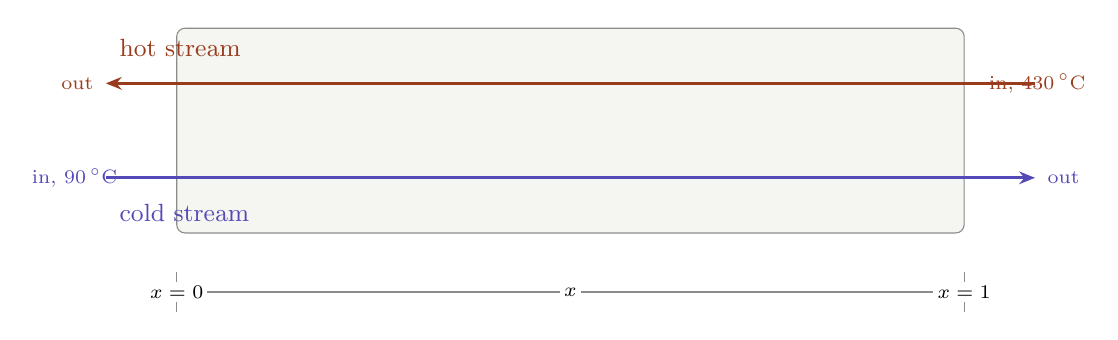
\begin{tikzpicture}[x=1cm,y=1cm]
  \draw[rounded corners=3pt, draw=black!45, fill=neut!60]
        (0,0) rectangle (10,2.6);
  \draw[ar, line width=1.1pt, warn]   (10.9,1.9) -- (-0.9,1.9);
  \draw[ar, line width=1.1pt, accent] (-0.9,0.7) -- (10.9,0.7);
  \node[font=\small, warn,   anchor=west] at (-0.85,2.35) {hot stream};
  \node[font=\small, accent, anchor=west] at (-0.85,0.25) {cold stream};
  \node[lbl, warn,   anchor=east] at (11.6,1.9) {in, \SI{430}{\celsius}};
  \node[lbl, warn,   anchor=east] at (-1.0,1.9)  {out};
  \node[lbl, accent, anchor=west] at (-1.9,0.7)  {in, \SI{90}{\celsius}};
  \node[lbl, accent, anchor=west] at (11.0,0.7)  {out};
  \draw[black!45] (0,-0.5) -- (0,-1.0);
  \draw[black!45] (10,-0.5) -- (10,-1.0);
  \draw[{Stealth[length=1.6mm]}-{Stealth[length=1.6mm]}, black!45]
        (0,-0.75) -- (10,-0.75);
  \node[lbl, fill=white, inner sep=1.5pt] at (0,-0.75)  {$x=0$};
  \node[lbl, fill=white, inner sep=1.5pt] at (10,-0.75) {$x=1$};
  \node[lbl, fill=white, inner sep=1.5pt] at (5,-0.75)  {$x$};
\end{tikzpicture}
\caption{A counterflow exchanger. The two streams run in opposite
directions, so ``which end'' means different things to each of them.}
\label{fig:cf}
\end{figure}

Figure~\ref{fig:cf} is the whole of it. Everything in this chapter is a
statement about a position along that box, so the coordinate has to be
nailed down before anything else.

Let $x$ run from the left end to the right end, \SI{0}{} to \SI{1}{},
regardless of which way either fluid happens to be travelling. Then:

\begin{center}
\begin{tabular}{@{}lll@{}}
\toprule
       & hot stream & cold stream \\
\midrule
$x=0$  & outlet     & inlet  \\
$x=1$  & inlet      & outlet \\
\bottomrule
\end{tabular}
\end{center}

Read that table twice, because it is the one thing that makes the rest of
the chapter either obvious or impenetrable. A single value of $x$ names one
cross-section of the metal. At that cross-section there is some hot fluid on
one side and some cold fluid on the other, and the hot fluid there is nearly
finished with its journey while the cold fluid there is just beginning its
own. They are at the same place and at opposite points in their respective
lives.

Two consequences follow immediately.

At $x=0$ the hot stream is as cold as it will get, and it is sitting next to
cold fluid that has not been warmed by anything yet. At $x=1$ the cold
stream is as hot as it will get, and it is sitting next to the hottest fluid
in the exchanger. So at both ends the exchanger is arranged so that the hot
side is still above the cold side --- which is precisely why counterflow is
used, and why a parallel-flow arrangement could never recover this much.

And $x$ is not a length. The exchanger is not uniform: some parts of it do
far more work per metre than others, as \S\ref{sec:ua} will show. $x$ is
simply ``how far along'', and in the solver it is specifically \emph{how
much of the total heat has been transferred so far}, which is a much more
convenient thing to count.

\section{How much heat can move at all}
\label{sec:qmax}

Before asking how good an exchanger is, ask what perfection would even look
like. That ceiling is $Q_{\max}$, and it comes from two separate limits that
have nothing to do with the hardware.

\subsection{The hot stream can only give up so much}

The hot stream enters at \SI{430}{\celsius}. How cold could it possibly
leave?

Not colder than \SI{90}{\celsius}, because \SI{90}{\celsius} is where the
cold stream comes in. Heat only runs downhill. The moment the hot stream
drops below the temperature of the coldest fluid available to receive heat,
there is nothing left to push the transfer. So:

\begin{center}
\emph{the hot stream's limiting outlet temperature is the cold stream's
inlet temperature.}
\end{center}

\noindent Its limiting outlet \emph{state} is therefore
$(P_{h,\mathrm{out}},\, T_{c,\mathrm{in}})$ --- outlet pressure, because
that is where the fluid will physically be, and the other stream's inlet
temperature. Look up both enthalpies and difference them:
\[
  Q_{h,\lim} = f_h \left[\, h_{h,\mathrm{in}}
  - h(P_{h,\mathrm{out}},\, T_{c,\mathrm{in}}) \,\right].
\]
Say this comes out to \SI{500}{\kilo\joule\per\kilogram}.

\subsection{The cold stream can only take so much}

Mirror image. The cold stream enters at \SI{90}{\celsius} and could not
possibly leave hotter than \SI{430}{\celsius}, because that is the hottest
fluid in the box. Its limiting outlet state is
$(P_{c,\mathrm{out}},\, T_{h,\mathrm{in}})$:
\[
  Q_{c,\lim} = f_c \left[\, h(P_{c,\mathrm{out}},\, T_{h,\mathrm{in}})
  - h_{c,\mathrm{in}} \,\right].
\]
Say this comes out to \SI{600}{\kilo\joule\per\kilogram}.

\subsection{Why the smaller one wins}

Both streams carry the same heat --- whatever leaves one enters the other.
So a duty of \SI{600}{} would require the hot stream to surrender
\SI{600}{\kilo\joule\per\kilogram}, and it only has \SI{500}{} to give
before it hits \SI{90}{\celsius}. It cannot be done:
\[
  Q_{\max} = \min(500,\, 600) = \SI{500}{\kilo\joule\per\kilogram}.
\]
The hot stream is \textbf{the limiting side} here, and the extra
\SI{100}{\kilo\joule\per\kilogram} of appetite on the cold side simply goes
unsatisfied.

Which side limits is worth knowing rather than just computing, because it
tells you what to change. A hot-limited exchanger does not improve if you
make it bigger --- it improves if you send less flow down the cold side, and
that single sentence is the entire motivation for the recompression layout.

\begin{caveat}[title={Caveat: $Q_{\max}$ needs infinite hardware}]
These limits come from the inlet states alone. Nothing about size, metal or
cost enters. Reaching $Q_{\max}$ would need an exchanger of infinite
conductance, so it is a ceiling to measure against, never a design target.
\end{caveat}

\begin{caveat}[title={Caveat: the lookup $h(P,T)$ is ambiguous in a two-phase region}]
Both limits ask ``what is the enthalpy at this pressure and that
temperature'', and inside a saturation dome that question has infinitely
many answers --- at \SI{10}{\kilo\pascal} and \SI{45.8}{\celsius}, water can
be liquid at \SI{192}{}, vapour at \SI{2584}{}, or any mixture between.

The fix is to notice the limit does not want ``the'' enthalpy, it wants the
\emph{extreme} one consistent with the constraint: cooling takes $h_f$,
heating takes $h_g$. sCO$_2$ never meets this, since the cycle stays above
the critical pressure, but a Rankine condenser would hit it on the first
call, so the guard is in.
\end{caveat}

\section{Effectiveness: the first of three languages}

With a ceiling in hand, the obvious way to describe a real exchanger is as a
fraction of it:
\[
  \varepsilon = \frac{Q}{Q_{\max}}, \qquad\text{so}\qquad
  Q = \varepsilon\, Q_{\max}.
\]
At $\varepsilon = 0.90$ and $Q_{\max} = \SI{500}{\kilo\joule\per\kilogram}$,
the duty is \SI{450}{\kilo\joule\per\kilogram}.

It is convenient because it is bounded, dimensionless and directly tied to
the ceiling. It also hides something, and the hiding matters.

$Q_{\max}$ is not a constant. It depends on both inlet states, which depend
on the rest of the cycle. So \SI{90}{\percent} in one cycle and
\SI{90}{\percent} in another are \emph{not the same exchanger} --- they are
the same fraction of two different ceilings. You cannot cost an exchanger
from $\varepsilon$, you cannot compare two cycles' hardware by it, and a
sweep that holds $\varepsilon$ fixed while changing pressure ratio is
quietly changing the exchanger at every point.

That limitation is the reason the other two languages exist.

\section{The temperature profile}

To say anything more than ``how much heat'', the temperature at every $x$ is
needed, not just at the ends.

\subsection{Enthalpy first, because it is the easy one}

Here is where the choice of $x$ pays off. If $x$ counts \emph{fraction of
duty transferred}, then by the time you reach position $x$, exactly $xQ$ of
heat has changed hands. Energy accounting then gives the enthalpy directly,
with no properties involved at all:

\begin{align*}
  h_c(x) &= h_{c,\mathrm{in}} + \frac{xQ}{f_c}
         &&\text{cold stream, has absorbed $xQ$ since its inlet at $x=0$}\\
  h_h(x) &= h_{h,\mathrm{out}} + \frac{xQ}{f_h}
         &&\text{hot stream, still has $xQ$ left to give before its outlet at $x=0$}
\end{align*}

Note the hot stream is built \emph{up} from its outlet rather than down from
its inlet. That is the table in Figure~\ref{fig:cf} doing its work: at $x=0$
the hot stream is at its outlet, so $h_h(0) = h_{h,\mathrm{out}}$, and it
gets hotter as $x$ grows.

Both expressions are straight lines in $x$. Enthalpy is linear here
\emph{by construction} --- it is linear because $x$ was defined to make it
so.

\subsection{Then temperature, which is where the physics re-enters}

Pressures are interpolated between the two ends, and then the property
library converts:
\[
  T_h(x) = T\!\left(P_h(x), h_h(x)\right), \qquad
  T_c(x) = T\!\left(P_c(x), h_c(x)\right), \qquad
  \Delta T(x) = T_h(x) - T_c(x).
\]

\textbf{And this is the step that bends everything.} The enthalpy lines are
straight; the temperature curves are not, because $T$ is not proportional to
$h$. The conversion factor is $c_p$, and for sCO$_2$ near the cold end $c_p$
is in the middle of a violent peak. A stream there absorbs large amounts of
enthalpy while barely changing temperature, so its temperature curve goes
nearly flat exactly where the other one does not.

Straight in $h$, bent in $T$. Everything awkward about this exchanger comes
from that one sentence.

\section{The pinch, and why it hides in the middle}
\label{sec:pinch}

$\Delta T(x)$ is the driving force at position $x$. Where it is large, heat
moves easily; where it is small, heat moves reluctantly; if it ever reaches
zero the design is impossible, and if it goes negative the model is claiming
heat flows uphill.

The smallest value anywhere is the \textbf{pinch}:
\[
  \Delta T_{\mathrm{pinch}} = \min_{0 \le x \le 1} \Delta T(x).
\]

With constant $c_p$ on both sides, both temperature curves would be straight
and the minimum would sit at one end --- which is why textbook treatments
check the two ends and stop. Here the curves bend, so they can approach each
other in the middle and open out again on either side. Tabulating a profile
makes it plain:

\begin{center}
\begin{tabular}{@{}lrrrrr@{}}
\toprule
$x$                          & 0.00 & 0.25 & 0.50 & 0.75 & 1.00 \\
\midrule
$T_h$ [\si{\celsius}]        & 115  & 186  & 254  & 336  & 430 \\
$T_c$ [\si{\celsius}]        &  90  & 172  & 245  & 320  & 400 \\
$\Delta T$ [\si{\kelvin}]    &  25  &  14  &   9  &  16  &  30 \\
\bottomrule
\end{tabular}
\end{center}

Both ends look comfortable --- \SI{25}{\kelvin} and \SI{30}{\kelvin}. The
real pinch is \SI{9}{\kelvin}, buried at the middle, and an end-point check
would have missed it by a factor of three. \textbf{This is why the solver
computes a hundred-point profile instead of a closed-form effectiveness
relation}, and the whole machinery of this chapter exists to make that
possible.

\section{How big the exchanger has to be}
\label{sec:ua}

Now the hardware question. Over a slice carrying $\mathrm{d}Q$ across a gap
$\Delta T$, the conductance needed is
\begin{equation}
  \mathrm{d}(UA) = \frac{\mathrm{d}Q}{\Delta T},
  \qquad\text{so}\qquad
  UA = \int_0^Q \frac{\mathrm{d}Q}{\Delta T(Q)}.
  \label{eq:ua}
\end{equation}
The integrand blows up as $\Delta T \to 0$, which is the whole story in one
symbol: \textbf{heat moved across a small gap is bought with a large amount
of metal.}

\subsection{Doing the integral}

Cut the duty into equal slices and use the log-mean gap across each, since
$\Delta T$ varies within a slice:
\[
  \Delta T_{lm,j} = \frac{\Delta T_j - \Delta T_{j-1}}
                         {\ln\!\left(\Delta T_j / \Delta T_{j-1}\right)},
  \qquad
  UA \approx \sum_j \frac{\Delta Q}{\Delta T_{lm,j}}.
\]

Take \SI{450}{\kilo\joule\per\kilogram} in three slices of \SI{150}{} each,
with gaps of \SI{25}{}, \SI{12}{}, \SI{14}{} and \SI{30}{\kelvin} at the
four boundaries:

\begin{center}
\begin{tabular}{@{}llrrr@{}}
\toprule
Slice & gap, in\,\textrightarrow\,out & $\Delta T_{lm}$ [\si{\kelvin}]
      & $\Delta Q / \Delta T_{lm}$ & share \\
\midrule
1 & \SIrange{25}{12}{\kelvin} & 17.7 &  8.5 & \SI{31}{\percent} \\
2 & \SIrange{12}{14}{\kelvin} & 13.0 & 11.6 & \SI{43}{\percent} \\
3 & \SIrange{14}{30}{\kelvin} & 21.0 &  7.2 & \SI{26}{\percent} \\
\midrule
  &                           &      & \textbf{27.2} & \\
\bottomrule
\end{tabular}
\end{center}

\noindent Each slice carries exactly one third of the heat. The middle one
--- the pinched one --- consumes \SI{43}{\percent} of the hardware to do it.
Push the pinch down from \SI{12}{} to \SI{4}{\kelvin} and that slice alone
triples.

So the pinch is not merely a feasibility check. \textbf{It is the price
tag}, and the few kelvin nearest the pinch are where most of the exchanger
physically is.

Units: dividing \si{\kilo\joule\per\kilogram} by \si{\kelvin} gives
conductance per unit mass flow, \SI{27.2}{\kilo\watt\per\kelvin} for every
\si{\kilogram\per\second}. At \SI{500}{\kilogram\per\second} that is
\SI{13600}{\kilo\watt\per\kelvin} of real exchanger.

\section{Three ways to specify one exchanger}
\label{sec:threespecs}

Everything so far has assumed the duty $Q$ was already known. Usually it is
not --- and the interesting part is that there are three different things
you might know instead.

\subsection{Why three, and not one}

The three quantities $\varepsilon$, $\Delta T_{\mathrm{pinch}}$ and $UA$ are
not independent. For a fixed pair of inlet states, raising the duty raises
$\varepsilon$, closes the pinch and demands more $UA$, all monotonically.
Fix any one and the other two follow.

So they are three languages describing the same object, and which one you
speak depends on what you actually know:

\begin{center}
\begin{tabular}{@{}lp{0.33\linewidth}p{0.36\linewidth}@{}}
\toprule
Language & The question it answers & Who talks this way \\
\midrule
$\varepsilon$ & How much of the available heat do I want back?
  & Early design, before hardware exists. Dostal, Kim. \\
pinch & How close may the streams approach?
  & When a minimum approach is a design rule. The ME 306 brief, Kim. \\
$UA$ & How much exchanger do I physically have?
  & Costing, retrofit, off-design. Wu. \\
\bottomrule
\end{tabular}
\end{center}

Four sources in the literature, three different conventions, identical
physics. That is why the solver accepts all three rather than picking one.

\subsection{Mode A --- effectiveness given}

The easy one, because it requires no searching at all.

\begin{enumerate}\itemsep2pt
\item Compute $Q_{\max} = \min(Q_{h,\lim},\, Q_{c,\lim}) =
      \SI{500}{\kilo\joule\per\kilogram}$.
\item $Q = \varepsilon\, Q_{\max} = 0.90 \times 500 =
      \SI{450}{\kilo\joule\per\kilogram}$. \emph{Done --- no iteration.}
\item Build the profile at that $Q$.
\item Read the pinch off it: \SI{9}{\kelvin}.
\item Integrate for $UA$: \SI{27.2}{\kilo\watt\per\kelvin} per
      \si{\kilogram\per\second}.
\end{enumerate}

\noindent \textbf{Given} $\varepsilon$ \quad\textbf{$\to$ out comes}
$Q$, pinch, $UA$.

\subsection{Mode B --- pinch given}

Now you want a minimum approach of \SI{20}{\kelvin}, and you do not know the
duty. Raising the duty closes the pinch, so there is a duty that produces
exactly \SI{20}{\kelvin} --- it just has to be found.

Search on $\varepsilon$, since it is conveniently bounded in $[0,1]$:

\begin{enumerate}\itemsep2pt
\item Guess $\varepsilon = 0.70$. Then $Q = \SI{350}{}$, build the profile,
      read the pinch: \SI{38}{\kelvin}. Too wide --- the streams are further
      apart than asked, so more heat can be moved.
\item Guess $\varepsilon = 0.85$. Then $Q = \SI{425}{}$, pinch
      \SI{14}{\kelvin}. Too tight --- overshot.
\item The answer is now trapped: $0.70 < \varepsilon < 0.85$.
\item Halve it. $\varepsilon = 0.775 \to \SI{24}{\kelvin}$, still wide, so
      the bracket becomes $0.775$--$0.85$.
\item $\varepsilon = 0.8125 \to \SI{18}{\kelvin}$, tight, bracket
      $0.775$--$0.8125$.
\item Continue until $\varepsilon = 0.80$ gives exactly
      \SI{20}{\kelvin}.
\end{enumerate}

Formally the loop is driving a residual to zero,
\[
  F(\varepsilon) = \Delta T_{\mathrm{pinch}}(\varepsilon)
                   - \Delta T_{\mathrm{target}} = 0,
\]
but the loop above \emph{is} the method, and the algebra is only a compact
way of writing it down. Note the sign: $F$ \emph{decreases} as $\varepsilon$
rises, which is the opposite of the usual convention and worth remembering
when reading the code.

\noindent \textbf{Given} pinch \quad\textbf{$\to$ searched for}
$\varepsilon$ \quad\textbf{$\to$ out comes} $Q$, $UA$.

\subsection{Mode C --- $UA$ given}

Same shape, different residual. You own an exchanger of
\SI{30}{\kilo\watt\per\kelvin} per \si{\kilogram\per\second} and want to
know what it achieves.

\begin{enumerate}\itemsep2pt
\item Guess $\varepsilon = 0.80$, build the profile, integrate:
      \SI{19}{}. Too small --- the hardware you own can do more.
\item Guess $\varepsilon = 0.90$: \SI{35}{}. Too large.
\item Bracketed. Converge to $\varepsilon = 0.855$, which needs exactly
      \SI{30}{}.
\item Read the pinch that results.
\end{enumerate}

\noindent \textbf{Given} $UA$ \quad\textbf{$\to$ searched for}
$\varepsilon$ \quad\textbf{$\to$ out comes} $Q$, pinch.

\subsection{All three at once}

\begin{center}
\begin{tabular}{@{}llll@{}}
\toprule
Mode & Given & Searched for & Falls out \\
\midrule
Effectiveness & $\varepsilon$ & --- (direct) & $Q$, pinch, $UA$ \\
Pinch & $\Delta T_{\mathrm{pinch}}$ & $\varepsilon$ & $Q$, $UA$ \\
Conductance & $UA$ & $\varepsilon$ & $Q$, pinch \\
\bottomrule
\end{tabular}
\end{center}

The profile construction, the property calls and the $UA$ integration are
\emph{byte-for-byte the same code} in all three. Only the residual differs:
\[
  \varepsilon = \varepsilon_{\mathrm{spec}},
  \qquad
  \Delta T_{\mathrm{pinch}}(\varepsilon) - \Delta T_{\mathrm{spec}} = 0,
  \qquad
  UA(\varepsilon) - UA_{\mathrm{spec}} = 0.
\]

That is the whole design. Three modes, one solver, one line of difference.

\section{Now the code}

Having worked through it by hand, the implementation should read as a
transcript of what you just did.

\subsection{The two limits, and their minimum}

\codefile[title={cycles/physics/hx\_limits.py}]{duty_limits.py}

\noindent Line for line: get both inlet temperatures from $(P,h)$; ask for
the hot stream's enthalpy at the \emph{cold} inlet temperature and the cold
stream's at the \emph{hot} inlet temperature; difference and scale by flow.
\code{limiting\_enthalpy} is the two-phase guard from
\S\ref{sec:qmax}. The caller takes the \code{min}.

\subsection{The profile}

\codefile[title={cycles/physics/hx\_profile.py}]{hx_profile.py}

\noindent The two enthalpy lines are the equations of the profile section,
unchanged. \code{h\_h} is built from \code{hot\_out\_h} upward, which is the
$x=0$-is-the-hot-outlet convention made concrete. Pressures interpolate ---
note \code{P\_h} runs from \code{P\_hot\_out} to \code{P\_hot\_in}, backwards
relative to the cold side, because the hot stream travels the other way. Two
property calls per node, which at \num{100} nodes is where essentially all
the runtime goes.

\subsection{The integration}

\codefile[title={cycles/physics/hx\_sizing.py}]{ua_sizing.py}

\noindent \code{lmtd} has two guards worth noting. A non-positive gap
returns \code{NaN} rather than a number, so a temperature cross propagates
out as an unmistakable failure instead of a plausible-looking $UA$. And when
the two gaps are nearly equal the log form is numerically unstable
($\ln 1 \approx 0$ divided into $\approx 0$), so it falls back to the
arithmetic mean, which is the correct limit anyway.

\subsection{The three modes}

\codefile[title={cycles/blocks/heat\_exchanger.py (excerpt)}]{hx_spec.py}

\noindent The comparison table above, in code. Each branch produces
\code{eps} and nothing else; everything after the \code{if} is shared.
\code{\_seek} is the root-finder --- a secant warm-started from the previous
outer iterate, falling back to bisection on the first call, for reasons that
belong in the chapter on solving the network rather than here. The
\code{NaN}\,\textrightarrow\,\code{1e30} substitution in the $UA$ branch is
how a crossed profile is told to the search: unreachable, push
$\varepsilon$ down.

\begin{caveat}[title={Caveat: the pressure interpolation is linear and that is a guess}]
Real pressure drop goes roughly as the square of velocity and varies with
density, so it is not linear along the exchanger. The error is small
because the total drop is a few percent of absolute pressure, but it is an
assumption, not a derivation.
\end{caveat}

\begin{caveat}[title={Caveat: a converged $UA$ is not a size}]
$UA$ is a conductance. Turning it into area needs $U$, into volume needs a
channel geometry, into mass needs a material --- and none of those are in
this program. Every ``compactness'' statement made from $UA$ alone is a
comparison between layouts using the same assumed technology, never an
absolute size.
\end{caveat}

\section{What to remember}

\begin{itemize}\itemsep2pt
\item The recuperator raises efficiency by shrinking the reactor's bill,
      not by producing more work.
\item $x$ is fraction-of-duty, and $x=0$ is the hot \emph{outlet} and the
      cold \emph{inlet}.
\item $Q_{\max} = \min(Q_{h,\lim},\, Q_{c,\lim})$, each limit found by
      cooling or heating one stream to the \emph{other} stream's inlet
      temperature.
\item Enthalpy is straight in $x$; temperature is bent, because $c_p$ varies.
      The pinch can therefore hide in the middle.
\item $UA = \int \mathrm{d}Q/\Delta T$, so the few kelvin around the pinch
      are where most of the metal is.
\item $\varepsilon$, pinch and $UA$ are three languages for one exchanger.
      Fix one, the other two follow. Only $UA$ is physical.
\end{itemize}

% =====================================================================
\chapter{Rejecting heat}
\label{ch:precooler}

Every cycle has to throw away the heat it did not turn into work, and this
chapter is about the hardware that does it. One block covers all of it. A
precooler brings the fluid back to the compressor inlet; an intercooler sits
between two compression stages; the partial cooling layout has two coolers
at two different pressures. They differ in where they sit and what flow they
carry, not in what they are.

That matters more than it sounds, because the cooling system turns out to be
the largest exchanger in the plant and the layouts change it substantially
--- in ways that reverse the hardware comparison a recuperator-only count
produces. Chapter~\ref{ch:splitting} uses the result; this chapter builds it.

\section{The smallest-looking component is the biggest}
\label{sec:biggest}

The precooler takes the turbine exhaust after the recuperator has recovered
what it can, and rejects the rest to cooling water. It sounds like the least
interesting box in the plant. By conductance it is the largest, and the
reason follows directly from two things already established.

The first is the specific-heat peak. The precooler works at the cold end of
the cycle, bringing \ce{CO2} down to \SI{32}{\celsius}, which is exactly
where $c_p$ is at its maximum. Heat released near a $c_p$ peak comes out
over a very small temperature change, so most of the precooler's duty is
transferred within a few degrees of the compressor inlet temperature.

The second is Equation~\eqref{eq:ua}, $UA = \int \mathrm{d}Q / \Delta T$.
The cooling water arrives at around \SI{25}{\celsius}. If most of the heat
is leaving the \ce{CO2} at around \SI{35}{\celsius}, then most of the
exchanger is working across a gap of about ten kelvin, and that integral
over such a gap is large.

Put those together: a great deal of duty, concentrated into a narrow
temperature band, dumped across a small gap. The precooler ends up needing
several times the conductance of the recuperator that
Chapter~\ref{ch:recup} spent eleven pages worrying about, and it demands
well over a tonne of cooling water per second for a plant producing a few
tens of megawatts of electricity.

Two consequences follow, and both are easy to get wrong.

\textbf{Any compactness claim that counts the recuperator and ignores the
precooler is wrong by a large factor.} The precooler is the bigger object.

\textbf{The cooling water is a siting constraint.} A reactor sold on being
deployable anywhere needs a river, a lake or a large cooling tower, and that
is a limit on where it can go rather than a detail of the heat balance.

\begin{figure}[htbp]
\centering
\begin{tikzpicture}
\begin{axis}[width=12cm, height=5.6cm,
  xlabel={Duty rejected [\si{\kilo\joule\per\kilogram}]},
  ylabel={Temperature [\si{\celsius}]},
  xmin=0, xmax=200, ymin=20, ymax=95,
  legend pos=north west, legend style={font=\small,draw=black!30},
  grid=both, grid style={black!8},
  tick label style={font=\small}, label style={font=\small}]
\addplot[warn, thick] table[x=Q,y=Thot] {data/precooler_profile.dat};
\addlegendentry{\ce{CO2}, \SI{7.7}{\mega\pascal}}
\addplot[accent, thick] table[x=Q,y=Tcold] {data/precooler_profile.dat};
\addlegendentry{cooling water, \SIrange{25}{35}{\celsius}}
\end{axis}
\end{tikzpicture}
\caption{The precooler against cooling water. The \ce{CO2} curve falls
steeply while the fluid is still gas-like, then flattens sharply near
\SI{35}{\celsius} as the specific-heat peak absorbs most of the duty over
very little temperature. Water, with an almost constant $c_p$, is a straight
line. One curve bends and the other does not, so the closest approach lands
roughly a third of the way along, inside the exchanger rather than at either
end. Same mechanism as the recuperator, same reason the precooler cannot be
sized from its end states.}
\label{fig:precooler}
\end{figure}

\section{How much water, or how big: pick one}
\label{sec:watertrade}

The water-side temperature rise is a free design variable, and it trades
directly against exchanger size. The trade runs like this.

Let the water warm more and you need less of it, because the same duty
divided by a larger $\Delta T$ needs a smaller flow. But the water curve in
Figure~\ref{fig:precooler} then climbs more steeply towards the flat
\ce{CO2} curve, so the gap between them narrows, and by
Equation~\eqref{eq:ua} a narrower gap means more conductance.

Less water, bigger exchanger. There is no setting that gives you both.

\begin{center}
\begin{tabular}{@{}rrrr@{}}
\toprule
Water $\Delta T$ [\si{\kelvin}] & Water flow [\si{\kilogram\per\second}]
  & Precooler $UA$ [\si{\kilo\watt\per\kelvin}] & Pinch [\si{\kelvin}] \\
\midrule
 5 & 3200 &  6000 & 7.0 \\
10 & 1600 &  7200 & 5.5 \\
15 & 1100 &  9300 & 3.8 \\
20 &  800 & 14000 & 1.9 \\
\bottomrule
\end{tabular}
\end{center}

\noindent (Rounded; the final report has the computed values and
the same trade read by water flow instead.)

Read the ends against each other. Going from \SI{10}{} to
\SI{20}{\kelvin} halves the water flow and nearly doubles the exchanger,
while squeezing the pinch down to \SI{1.9}{\kelvin}, which is too tight to
build or to operate with any margin. Somewhere around
\SIrange{10}{15}{\kelvin} is the usable band, and that table is the whole
argument for choosing within it.

\section{What more water actually buys}
\label{sec:watersweep}

The table above varies the water's temperature rise. It is more direct to
vary the water flow itself, which is what \code{coolant\_flow} is for, and
doing so turns up something the first table hides.

\begin{center}
\begin{tabular}{@{}rrrrrr@{}}
\toprule
Water & $T_{w,\text{out}}$ & Pinch & Pinch at & $UA$ & $UA$ vs \\
{[\si{\kilogram\per\second}]} & [\si{\celsius}] & [\si{\kelvin}] & $x$
  & [\si{\kilo\watt\per\kelvin}] & recuperator \\
\midrule
 854 & 43.9 & 2.36 & 0.39 & 12444 & 7.5 \\
1195 & 38.5 & 4.34 & 0.35 &  8474 & 5.1 \\
1610 & 35.0 & 5.50 & 0.32 &  7191 & 4.3 \\
2220 & 32.3 & 6.33 & 0.29 &  6464 & 3.9 \\
2732 & 30.9 & 6.71 & 0.27 &  6166 & 3.7 \\
3415 & 29.7 & 7.00 & 0.00 &  5933 & 3.6 \\
4439 & 28.6 & 7.00 & 0.00 &  5736 & 3.4 \\
\bottomrule
\end{tabular}
\end{center}

Follow the ``pinch at'' column down. For most of the table the closest
approach is \emph{inside} the exchanger, around a third of the way along,
and it widens steadily as water is added. Then at about
\SI{3400}{\kilogram\per\second} it jumps to $x = 0$, the cold end, and stops
at \SI{7.00}{\kelvin} exactly.

That number is not a coincidence. The \ce{CO2} leaves at
\SI{32}{\celsius} and the water arrives at \SI{25}{\celsius}, so
\SI{7}{\kelvin} is the gap between the two terminal temperatures, and no
amount of water can open it further. \textbf{Past that point extra water
buys nothing}: the approach is capped by where the two streams start and
finish, not by the flow. The conductance keeps falling slightly, but with
diminishing returns and a cooling-water bill that keeps rising.

So the usable range has a hard edge at one end and a practical one at the
other: below roughly \SI{1000}{\kilogram\per\second} the pinch is too tight
to build, and above roughly \SI{3000}{} the water is being supplied for no
benefit.

\subsection{Water flow does not change the efficiency}

One column is missing from that table because it would be identical all the
way down. $\eta_{th}$ is \SI{32.720}{\percent} in every row.

That is worth stating because the opposite is the natural assumption. The
cycle was solved to a \ce{CO2} outlet temperature the case specified, so the
water side never touches the thermodynamics. It decides what the heat sink
\emph{costs}, not what the cycle \emph{achieves}.

The link back to efficiency is real but indirect, and runs the other way. If
the available water could not bring the \ce{CO2} to \SI{32}{\celsius} at any
sane exchanger size, the compressor inlet temperature would have to rise,
and \emph{that} would cost efficiency --- quite a lot of it, since
Chapter~\ref{ch:work} showed how much the cycle depends on compressing near
the critical point. This solver works in the opposite direction: you assert
\SI{32}{\celsius} and it reports what the water must do to deliver it. A
flagged pinch is how it tells you the assertion was unreasonable.

\begin{caveat}[title={Caveat: the coolant side still does not feed back}]
It computes water flow, pinch and conductance from a duty that was
\emph{already} decided by the \ce{CO2} outlet temperature you specified. It
does not feed back into the cycle.

\textbf{What it costs:} if the water cannot achieve that outlet temperature,
you get a flagged pinch rather than a corrected cycle. The solver tells you
a design is impossible; it does not find you a possible one.
\end{caveat}

\begin{caveat}[title={Caveat: cooling-water pumping power is not modelled, deliberately}]
Moving \SI{1610}{\kilogram\per\second} of water costs real shaft power, and
that power comes off the plant's output. It is not computed here, and the
reason is worth recording because it was a decision rather than an
oversight.

Pump work is $\dot m \Delta P / (\rho\, \eta)$, and the flow is known. The
pressure drop is not. Getting it honestly needs the exchanger's channel
geometry --- diameter, length, channel count --- and this project never
computes geometry: Chapter~\ref{ch:sizing} gets as far as conductance and
stops, because $U$ is not modelled. So any $\Delta P$ would be an assumption
wearing the costume of a result, and worse, a Darcy--Weisbach calculation
would be using a geometry that has no connection to the $UA$ reported beside
it. The two could contradict each other with nothing to catch it.

\textbf{What it costs, and it is not small.} Dostal found that including
pumping \emph{shifts the optimum pressure ratio}, because water demand
spikes in exactly the near-critical region where the cycle most wants to
operate. The property that makes the compressor cheap is the one that makes
the precooler expensive, and the two optima do not coincide. So any optimum
pressure ratio from this project is wrong in a known direction, and the
honest fix is a real exchanger sizing model rather than a plausible number.
\end{caveat}

\section{One block, four coolers}
\label{sec:coolerblock}

Nothing above was specific to a precooler. A cooler rejecting heat to an
external supply is a counterflow exchanger whose cold stream leaves the
cycle instead of coming back round, and that is true wherever it sits.

So the sizing lives in \code{physics/coolant.py}, below the blocks, and the
cooler block is thin. If it lived inside the cooler, a second cooler in the
same layout would either duplicate it or force a special case, and the
entire architecture rests on blocks being interchangeable.

\subsection{The same pattern as the recuperator}

\S\ref{sec:threespecs} showed three ways to specify one exchanger, all
collapsing to an effectiveness before any profile was built. The coolant
side has four ways to specify one supply, all collapsing to a coolant flow:

\codefile[title={cycles/specs.py}]{coolant_specs.py}

\begin{center}
\begin{tabular}{@{}lp{0.52\linewidth}@{}}
\toprule
Spec & The question it answers \\
\midrule
\code{CoolantFlow}    & What do I get for this much coolant? \\
\code{CoolantOutlet}  & How much coolant to send it out at this temperature? \\
\code{CoolantRise}    & How much coolant to warm it by this much? \\
\code{CoolantPinch}   & How much coolant to hold this approach? \\
\bottomrule
\end{tabular}
\end{center}

Only the first answers a question a sweep can ask. The other three each
demand an outcome and report what it costs; \code{CoolantFlow} supplies a
resource and reports what it buys, which is the direction a design study
runs in.

\codefile[title={cycles/physics/coolant.py}]{coolant_size.py}

\section{What the coolant costs to move}
\label{sec:pumping}

Pushing a tonne of water a second through an exchanger costs shaft power,
and that power comes off the plant's output. For an incompressible fluid it
is Equation~\eqref{eq:vdp} with $v$ genuinely constant:
\[
  \dot W_{\text{pump}} = \frac{\dot m\, \Delta P}{\rho\, \eta_{\text{pump}}}.
\]
The flow is known. $\Delta P$ is the problem, and how this project handles
it is a decision worth recording rather than a detail.

\subsection{Stated, never derived}

A geometry-based model was written here and removed. Darcy--Weisbach, taking
channel diameter, length and count, computing a Reynolds number and a
friction factor. The arithmetic was fine. The problem was that this project
computes $UA$ and never computes geometry (Chapter~\ref{ch:sizing}), so the
geometry handed to such a model has no connection to the $UA$ reported
beside it, and nothing can check the two against each other. You could
specify a channel count that could not possibly deliver the conductance in
the same table and get a confident pressure drop for an exchanger that
cannot exist.

\begin{choicebox}
\textbf{The solver applies a pressure drop you state; it never manufactures
one.} A number that looks derived but is invented is worse than an
assumption clearly labelled as one, because only the first gets quoted
without its caveat.

\code{NoPumping} is the default and reports zero rather than a guess.
\code{FixedDrop} takes a loss in pascals. \code{QuadraticDrop} scales that
loss as the square of flow, anchored at a point you know.
\end{choicebox}

\codefile[title={cycles/physics/hydraulics.py}]{circuit_models.py}

Two things about that module. The drops are in \textbf{pascals}, not
fractions of the operating pressure --- hydraulic loss is set by dynamic
pressure and geometry, and a circuit at \SI{2}{bar} loses the same across
the same exchanger as one at \SI{6}{bar}. Making it fractional would
understate it roughly fiftyfold and, worse, would let an optimiser reduce
pumping power by lowering the circuit pressure, which is not a thing.

And the quadratic option matters more than its magnitude. Loss goes as the
square of velocity, so pump work goes as the \emph{cube} of flow. A fixed
drop makes it linear. That exponent, not the \SI{100}{\kilo\pascal}, is what
decides whether a coolant-flow sweep has an interior optimum.

\subsection{What it costs, on the baseline}

\begin{center}
\begin{tabular}{@{}rrrrr@{}}
\toprule
Water [\si{\kilogram\per\second}] & $UA$ [\si{\kilo\watt\per\kelvin}]
  & Pump [\si{\kilo\watt}] & $\eta_{th}$ [\si{\percent}]
  & $\eta$ net of pump [\si{\percent}] \\
\midrule
 854 & 12450 &   30 & 32.720 & 32.690 \\
1195 &  8476 &   83 & 32.720 & 32.637 \\
1610 &  7191 &  202 & 32.720 & 32.518 \\
2220 &  6464 &  529 & 32.720 & 32.191 \\
3415 &  5933 & 1926 & 32.720 & 30.794 \\
\bottomrule
\end{tabular}
\end{center}

$\eta_{th}$ does not move, because pump work is an auxiliary load and not
cycle work. $\eta$ net of pump falls monotonically as water is added, which
means efficiency \emph{still} cannot choose a coolant flow: pump work is a
pure cost with no efficiency benefit to trade against, and the exchanger
that pushes back the other way is hardware, invisible to a first-law
efficiency. The trade is between a cooling bill and a capital cost, and it
is settled outside thermodynamics.

\section{Every layout's heat sink}
\label{sec:everysink}

The precooler is the larger exchanger in every layout, not the
recuperator, and the reason is \S\ref{sec:biggest}: it rejects more heat
across a far smaller temperature difference.

\begin{center}
\small
\begin{tabular}{@{}llrrrrr@{}}
\toprule
Layout & Cooler & Duty [MW] & Water [kg/s] & Pinch [K] & $UA$ & Pump [kW] \\
\midrule
recuperated & COOLER & 63.5 & 1519 & 4.90 & 8419 & 0 \\
recompression & PC & 57.8 & 1382 & 4.90 & 7662 & 61 \\
partial cooling & PC1 & 21.8 & 521 & 7.00 & 1484 & 5 \\
 & PC2 & 37.9 & 908 & 4.12 & 6425 & 28 \\
 & \emph{total} & --- & 1429 & --- & 7909 & 33 \\
intercooled & IC & 11.9 & 284 & 4.52 & 1997 & 1 \\
 & PC & 51.9 & 1242 & 4.13 & 8761 & 79 \\
 & \emph{total} & --- & 1526 & --- & 10758 & 80 \\
\bottomrule
\end{tabular}

\end{center}
\from{cooling/per_cooler.csv}{python -m project.studies.cooling}

Three things that table says and prose cannot.

\textbf{Recompression's precooler is \emph{smaller} than the
baseline's} --- \SI{7662}{} against \SI{8419}{\kilo\watt\per\kelvin} ---
even though the layout is far more elaborate. Two reasons: it rejects
less heat per megawatt, because the recuperators recover more of it; and
the precooler carries only the unsplit fraction of the flow. This is why
a conductance comparison that counts recuperators alone is misleading
(\S\ref{sec:totalua}).

\textbf{The pinch sticks at \SI{7.00}{\kelvin}} wherever the \ce{CO2}
outlet is \SI{32}{\celsius} and the water supply is
\SI{25}{\celsius}. That floor is the difference between those two
temperatures and no amount of water opens it further.

\textbf{Intercooling adds \SI{2339}{\kilo\watt\per\kelvin} of cooler}
on top of its extra recuperator, which is the hardware cost of a layout
that also loses on efficiency.

\section{What to remember}

\begin{itemize}\itemsep2pt
\item The cooling system is the largest exchanger in the plant, because it
      works where $c_p$ peaks and across a small gap to the coolant.
\item Its pinch is internal, for the same reason the recuperator's is, and
      it saturates at
      $T_{\text{out}} - T_{\text{coolant,in}}$ once coolant is plentiful.
\item One block covers every cooler. The sizing lives below the blocks,
      because several layouts have more than one.
\item Four coolant specs, all collapsing to a flow, mirroring the three
      exchanger specs collapsing to an effectiveness.
\item Pressure drops are \emph{stated in pascals, never derived}: this
      project computes $UA$ and not geometry, so a geometry-based drop would
      describe an exchanger unrelated to the one being sized.
\item Pump work goes as the cube of flow when the drop scales properly, and
      it is an auxiliary load: it never enters $\eta_{th}$.
\item Efficiency cannot choose a coolant flow. The exchanger that pushes
      back is hardware, and hardware is invisible to a first-law efficiency.
\item Recompression needs the \emph{least} cooling water of the four
      layouts, which the efficiency table gives no hint of.
\end{itemize}
\chapter{The layouts}
\label{ch:splitting}

\section{Capacity rate}
\label{sec:capacityrate}

One idea has to be clear before either layout in this chapter makes any
sense, and it is not in the Brayton formula sheet.

The \textbf{capacity rate} of a stream is
\[
  C = \dot m \, c_p,
\]
which is how much heat it swallows, or gives up, per kelvin of temperature
change. Units of \si{\kilo\watt\per\kelvin}. A stream with a large $C$ moves
its temperature reluctantly; a stream with a small $C$ moves it easily.

\subsection{When the two sides match}

Put two streams in a counterflow exchanger with $C_{\text{hot}} =
C_{\text{cold}} = \SI{5}{\kilo\watt\per\kelvin}$ and transfer
\SI{100}{\kilo\watt}.

The hot stream loses \SI{100}{\kilo\watt} and therefore cools by
$100/5 = \SI{20}{\kelvin}$. The cold stream gains the same
\SI{100}{\kilo\watt} and warms by $100/5 = \SI{20}{\kelvin}$. They move by
the same amount, so \textbf{the gap between them does not change}.

Do that slice by slice along the whole exchanger and the two temperature
curves stay parallel. The gap is the same everywhere, and by
Equation~\eqref{eq:ua} every part of the exchanger is working equally hard.
Nothing is wasted and nothing pinches. This is the arrangement the textbook
$\varepsilon$--NTU relations are usually taught with, and it is the best
case.

\subsection{When they do not}

Now unbalance it. Keep $C_{\text{hot}} = \SI{5}{}$ but make
$C_{\text{cold}} = \SI{10}{\kilo\watt\per\kelvin}$, and transfer the same
\SI{100}{\kilo\watt}.

The hot stream still cools by \SI{20}{\kelvin}. The cold stream, now twice
as reluctant, warms by only $100/10 = \SI{10}{\kelvin}$. The hot curve has
fallen twice as fast as the cold curve has risen, so \textbf{the gap has
closed by \SI{10}{\kelvin}} across that one slice.

Repeat down the exchanger and the two curves converge. Somewhere they come
closest, and by Equation~\eqref{eq:ua} that somewhere is where almost all
the metal has to go. Push it a little further and they touch, and the design
is impossible.

\subsection{Which is exactly the position sCO$_2$ puts itself in}

Both sides of the recuperator carry the same fluid at the same mass flow,
so $\dot m$ is equal. But they are at different pressures, and
Figure~\ref{fig:cp} showed that $c_p$ at \SI{20}{\mega\pascal} and $c_p$ at
\SI{7.7}{\mega\pascal} are not the same function.

Near the cold end of the recuperator the high-pressure stream is sitting on
the shoulder of its specific-heat peak, with a $c_p$ roughly \num{1.75}
times that of the low-pressure stream at the same point. Equal $\dot m$,
unequal $c_p$, so unequal $C$. The cold side is the reluctant one, the
curves converge, and the exchanger pinches.

And the damage does not stop at the exchanger. Once the profile pinches, no
more heat can be moved, so the hot stream leaves the recuperator warmer than
it ought to be. That extra heat goes to the precooler and is thrown into a
river. \textbf{The pinch caps recuperation, and recuperation is what caps
efficiency.}

\section{Recompression}

\subsection{The only lever left}

$c_p$ is a property of the fluid and will not negotiate. The capacity rate
is $\dot m c_p$. So if the cold side has too much capacity rate, the only
remaining move is to \textbf{put less mass through it}.

Split the flow after the low-temperature recuperator. Send a fraction
$(1-x)$ onward through the precooler and the main compressor as usual, and
let only that reduced flow pass up the cold side of the exchanger. Choose
$x$ so that
\[
  (1-x)\, c_{p,\mathrm{HP}} \approx c_{p,\mathrm{LP}},
\]
and the capacity rates come back together, the curves stay parallel, and
the pinch opens up.

If the mismatch were \num{1.75} everywhere, the arithmetic would say remove
about \SI{43}{\percent} of the flow. It is not: the mismatch is that severe
only near the cold end and much milder further up, so the best compromise
across the whole exchanger sits lower, nearer \num{0.3}.

\subsection{Where the removed fluid goes}

It still has to get back to high pressure, and the route is the clever part.

Rather than following the rest through the precooler, the removed fraction
is compressed \emph{warm} by a second compressor and rejoins the main flow
after the low-temperature recuperator. It therefore bypasses both the
precooler and the exchanger whose balance it was spoiling. Above the mixing
point the full flow is restored and passes through the high-temperature
recuperator, where the specific heats are similar anyway and there was never
a mismatch to fix.

\begin{figure}[htbp]
\centering
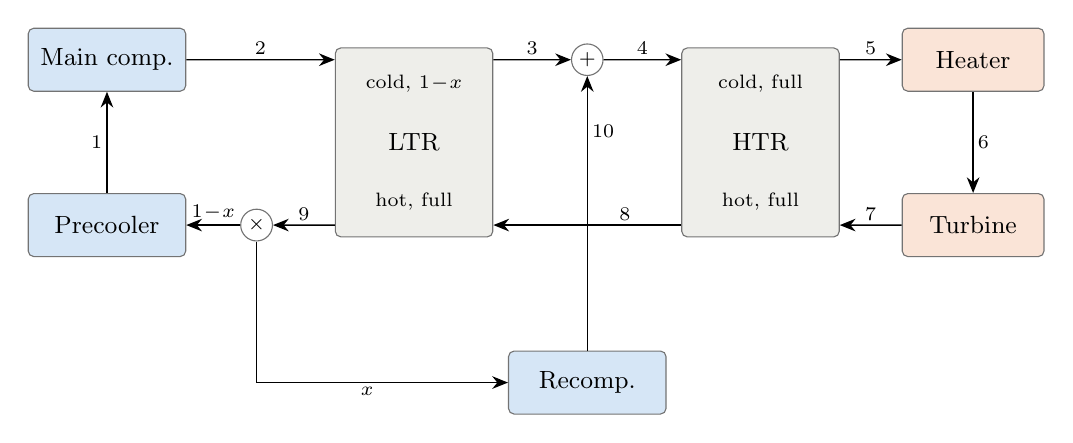
\begin{tikzpicture}[x=1cm,y=1cm]
  \node[coldblk, minimum width=20mm] (mc)   at (0,3.0)  {Main comp.};
  \node[coldblk, minimum width=20mm] (pc)   at (0,0.9)  {Precooler};
  \node[circle,draw=black!55,inner sep=1.2pt,font=\scriptsize] (spl) at (1.9,0.9) {$\times$};
  \node[neutblk, minimum height=24mm, minimum width=20mm] (ltr) at (3.9,1.95) {};
  \node[font=\scriptsize] at (3.9,2.70) {cold, $1\!-\!x$};
  \node[font=\small]      at (3.9,1.95) {LTR};
  \node[font=\scriptsize] at (3.9,1.20) {hot, full};
  \node[circle,draw=black!55,inner sep=1.2pt,font=\scriptsize] (mix) at (6.1,3.0) {$+$};
  \node[neutblk, minimum height=24mm, minimum width=20mm] (htr) at (8.3,1.95) {};
  \node[font=\scriptsize] at (8.3,2.70) {cold, full};
  \node[font=\small]      at (8.3,1.95) {HTR};
  \node[font=\scriptsize] at (8.3,1.20) {hot, full};
  \node[hotblk, minimum width=18mm] (heat) at (11.0,3.0) {Heater};
  \node[hotblk, minimum width=18mm] (turb) at (11.0,0.9) {Turbine};
  \node[coldblk, minimum width=20mm] (rc)  at (6.1,-1.1) {Recomp.};

  \coordinate (lci) at ($(ltr.west)+(0,1.05)$);
  \coordinate (lco) at ($(ltr.east)+(0,1.05)$);
  \coordinate (lhi) at ($(ltr.east)+(0,-1.05)$);
  \coordinate (lho) at ($(ltr.west)+(0,-1.05)$);
  \coordinate (hci) at ($(htr.west)+(0,1.05)$);
  \coordinate (hco) at ($(htr.east)+(0,1.05)$);
  \coordinate (hhi) at ($(htr.east)+(0,-1.05)$);
  \coordinate (hho) at ($(htr.west)+(0,-1.05)$);

  \draw[ar] (pc)  -- node[lbl,left]{1} (mc);
  \draw[ar] (mc)  -- node[lbl,above]{2} (lci);
  \draw[ar] (lco) -- node[lbl,above]{3} (mix);
  \draw[ar] (mix) -- node[lbl,above]{4} (hci);
  \draw[ar] (hco) -- node[lbl,above]{5} (heat);
  \draw[ar] (heat) -- node[lbl,right]{6} (turb);
  \draw[ar] (turb) -- node[lbl,above]{7} (hhi);
  \draw[ar] (hho) -- node[lbl,above,pos=0.30]{8} (lhi);
  \draw[ar] (lho) -- node[lbl,above]{9} (spl);
  \draw[ar] (spl) -- node[lbl,above]{$1\!-\!x$} (pc);
  \draw[ar] (spl) |- node[lbl,below,pos=0.72]{$x$} (rc);
  \draw[ar] (rc)  -- node[lbl,right,pos=0.80]{10} (mix);
\end{tikzpicture}

\caption{Recompression. The low-temperature recuperator carries full flow on
its hot side and only $(1-x)$ on its cold side, which is what brings the
capacity rates together. Note what this does to the dependency structure:
the LTR needs a hot inlet the HTR produces, the HTR needs a cold inlet that
comes through the mixer, and the mixer needs the LTR's own outlet. The
dependency runs in a circle, which the simple recuperated layout never did.}
\label{fig:recompression}
\end{figure}

\subsection{In the solver, this is a list}

\codefile[title={project/layouts/recompression.py}]{layout_recompression.py}

\noindent No numbers, no physics, no equations. Only which blocks exist and
which streams join them. Partial cooling, below, is a different list of the
same block types, which is why adding it required no changes to the solver
at all.

\subsection{Why $x$ has an optimum rather than a limit}
\label{sec:xopt}

If recompression only fixed the pinch, you would push $x$ as high as
capacity-rate matching allowed and stop there. It does not, because the
recompressor is expensive in a way the main compressor is not.

Go back to Equation~\eqref{eq:vdp}, $w = \int v\,\mathrm{d}P$. The main
compressor works on fluid at \SI{32}{\celsius}, dense and nearly
incompressible, so $v$ in that integral is small. The recompressor works on
fluid that skipped the precooler: warm, and several times less dense. Say
the main compressor sees an average
\SI{0.002}{\metre\cubed\per\kilogram} and the recompressor sees
\SI{0.006}{}. Over the same pressure rise, the recompressor costs three
times as much per kilogram it handles.

So two effects pull in opposite directions as $x$ rises. Capacity-rate
matching improves, recovering more heat and shrinking the reactor's bill.
Recompressor work grows, spending more of the turbine's output. The two
cross, and the crossing is the optimum. It usually lands near $x = 0.3$;
Kim reports \num{0.307} for a comparable cycle.

The back-work ratio is where this shows up in the results. Switching
recompression on raises it from roughly \num{0.18} to roughly \num{0.27},
which is the recompressor handing back about a tenth of the turbine's
output in exchange for the recuperation it unlocked.

\begin{caveat}[title={Caveat: the split fraction is an input here, not a result}]
Dostal computes $x$ from a closure condition at the recompressor inlet. This
solver takes it as given and expects you to sweep it. Both are legitimate
and they answer different questions.

\textbf{What it costs:} you must say which you are reporting. An $x$ swept
to an optimum and an $x$ that fell out of a closure condition are not the
same claim, and quoting one as the other would be misleading.
\end{caveat}

\section{Partial cooling}

Partial cooling attacks the same problem from a different direction. It is
worth going slowly here, because the layout is easy to misread as
recompression with extra parts, and because the result most often quoted
about it belongs to a different cycle.

\subsection{What changes}

Two things.

First, the turbine is allowed to exhaust to a pressure \emph{below} the main
compressor inlet, with a pre-compressor afterwards to bring it back up. The
cycle therefore has three pressure levels instead of two.

Second, there are two coolers. The first takes the turbine exhaust down
before the pre-compressor; the second cools only the fraction that goes on
to the main compressor.

\subsection{The name is misleading, so read it carefully}
\label{sec:pcname}

Partial cooling \emph{also} splits the flow and recompresses part of it, and
the figure below shows that. On first sight it therefore looks like
``recompression with extra bits bolted on'', which is the natural reading
and the wrong one.

The split is not an addition. It is part of the layout as Angelino defined
it, and Dostal's description of that layout is explicit: only a fraction of
the working fluid goes to the main compressor, and the rest is compressed in
a recompressing compressor to the high-temperature recuperator inlet, where
the two merge. He gives the same reason for it that
\S\ref{sec:capacityrate} gives: the reduced flow on the high-pressure side
of the low-temperature recuperator equalises the capacity rates, so the
pinch does not occur.

The name is what misleads. \textbf{``Partial'' describes the flow, not the
cooling}: only \emph{part} of the fluid is cooled all the way down to the
main compressor inlet temperature. The rest is cooled once, in the first
cooler, and then recompressed warm.

It helps to see where this layout sits among its neighbours, all four of
which come from the same two papers.

\begin{center}
\begin{tabular}{@{}lccc@{}}
\toprule
Layout & Pressure levels & Flow split & Recuperators \\
\midrule
recuperated                  & 2 & no  & 1 \\
intercooled                  & 2 & no  & 1 (+ intercooler) \\
pre-compression              & 3 & no  & 2 \\
recompression                & 2 & yes & 2 \\
partial cooling              & 3 & yes & 2 \\
\;\;\dots with improved regeneration & 3 & yes & 3 (one three-stream) \\
\bottomrule
\end{tabular}
\end{center}

Recompression and partial cooling differ in exactly one column: the number
of pressure levels. That is the honest statement of what separates them, and
it is why the low-pressure level is the only thing worth sweeping to tell
them apart.

If you want the layout that is genuinely ``three pressure levels without a
split'', that is the \textbf{pre-compression} cycle, and it is a different
machine rather than a stripped-down partial cooling. Its compressor sits
\emph{between} the two recuperators on the hot side with no cooler before
it, so what it exploits is that compressing the stream raises both its
temperature and its specific heat, letting regeneration carry on past the
point where it would otherwise have stalled. It is not implemented here.

\subsection{Why that helps}

Carnot's result says a cycle improves when the average temperature at which
it rejects heat goes down, and partial cooling lowers that average twice
over. The first portion of heat is rejected at a genuinely lower
temperature, and the second portion is rejected from only a fraction of the
flow, so it carries less weight in the average.

The pinch improves too, for the same capacity-rate reason as recompression,
because the low-temperature recuperator's cold side again carries reduced
flow.

\subsection{What Dostal actually found, which is not what gets quoted}
\label{sec:dostal}

The result usually repeated is that partial cooling beats recompression
below \SI{20}{\mega\pascal} and loses above it. That is close enough to be
dangerous, and it is worth getting exactly right, because the layout that
wins is \emph{not} the one drawn above.

What Angelino compared, and Dostal reports, is that recompression achieves
the highest efficiency at turbine inlet pressures around
\SI{20}{\mega\pascal}, while at lower pressures the best of the set is
\textbf{partial cooling with improved regeneration}. That is a further
variant again: it adds a third recuperator carrying three streams, and
merges both precoolers into a single three-stream unit with the cooling
water. Plain partial cooling, the layout modelled here, sits between the two
in both complexity and efficiency.

The \emph{reason} Dostal gives for the crossover does carry over to the
plain layout, because it is a statement about pressure levels rather than
about recuperators: once the turbine exhaust pressure is no longer tied to
the main compressor inlet pressure, it becomes a free design variable, and
that freedom is worth more when the maximum pressure is low.

So the direction of the effect applies here. The magnitude does not.

\begin{caveat}[title={Caveat: the measured comparison does not test Angelino's crossover}]
The layout comparison in this project is recuperated against recompression
against \emph{plain} partial cooling, all at \SI{20}{\mega\pascal} with an
unswept low-pressure level. Angelino's claim is about a more complex layout
across a range of pressures.

\textbf{What it costs:} nothing computed here confirms or contradicts the
published crossover, and saying otherwise would be the easiest mistake in
the whole report to make. Testing it properly needs the third recuperator,
a three-stream exchanger model the solver does not have, and a sweep over
turbine inlet pressure.
\end{caveat}

\begin{figure}[htbp]
\centering
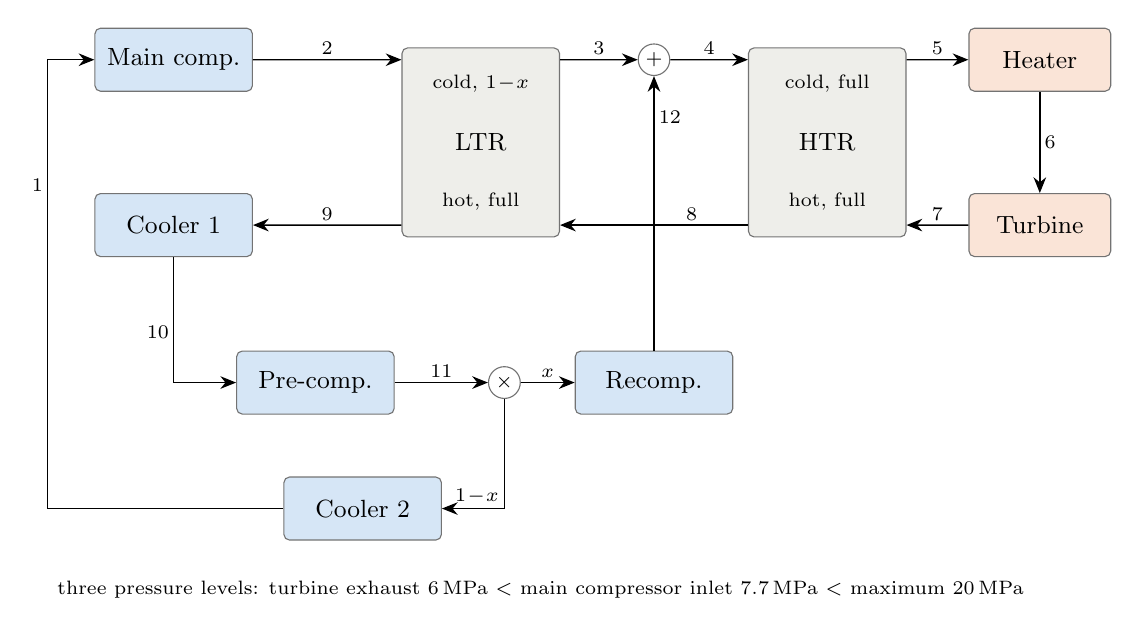
\begin{tikzpicture}[x=1cm,y=1cm]
  \node[coldblk, minimum width=20mm] (mc)    at (0,3.0)    {Main comp.};
  \node[coldblk, minimum width=20mm] (pc1)   at (0,0.9)    {Cooler 1};
  \node[coldblk, minimum width=20mm] (pcomp) at (1.8,-1.1) {Pre-comp.};
  \node[circle,draw=black!55,inner sep=1.2pt,font=\scriptsize] (spl) at (4.2,-1.1) {$\times$};
  \node[coldblk, minimum width=20mm] (rc)    at (6.1,-1.1) {Recomp.};
  \node[coldblk, minimum width=20mm] (pc2)   at (2.4,-2.7) {Cooler 2};

  \node[neutblk, minimum height=24mm, minimum width=20mm] (ltr) at (3.9,1.95) {};
  \node[font=\scriptsize] at (3.9,2.70) {cold, $1\!-\!x$};
  \node[font=\small]      at (3.9,1.95) {LTR};
  \node[font=\scriptsize] at (3.9,1.20) {hot, full};

  \node[circle,draw=black!55,inner sep=1.2pt,font=\scriptsize] (mix) at (6.1,3.0) {$+$};

  \node[neutblk, minimum height=24mm, minimum width=20mm] (htr) at (8.3,1.95) {};
  \node[font=\scriptsize] at (8.3,2.70) {cold, full};
  \node[font=\small]      at (8.3,1.95) {HTR};
  \node[font=\scriptsize] at (8.3,1.20) {hot, full};

  \node[hotblk, minimum width=18mm] (heat) at (11.0,3.0) {Heater};
  \node[hotblk, minimum width=18mm] (turb) at (11.0,0.9) {Turbine};

  \coordinate (lci) at ($(ltr.west)+(0,1.05)$);
  \coordinate (lco) at ($(ltr.east)+(0,1.05)$);
  \coordinate (lhi) at ($(ltr.east)+(0,-1.05)$);
  \coordinate (lho) at ($(ltr.west)+(0,-1.05)$);
  \coordinate (hci) at ($(htr.west)+(0,1.05)$);
  \coordinate (hco) at ($(htr.east)+(0,1.05)$);
  \coordinate (hhi) at ($(htr.east)+(0,-1.05)$);
  \coordinate (hho) at ($(htr.west)+(0,-1.05)$);

  % cold / high-pressure path, left to right
  \draw[ar] (mc)  -- node[lbl,above]{2} (lci);
  \draw[ar] (lco) -- node[lbl,above]{3} (mix);
  \draw[ar] (mix) -- node[lbl,above]{4} (hci);
  \draw[ar] (hco) -- node[lbl,above]{5} (heat);
  \draw[ar] (heat) -- node[lbl,right]{6} (turb);

  % hot / low-pressure path, right to left
  \draw[ar] (turb) -- node[lbl,above]{7} (hhi);
  \draw[ar] (hho)  -- node[lbl,above,pos=0.30]{8} (lhi);
  \draw[ar] (lho)  -- node[lbl,above]{9} (pc1);

  % down to the intermediate pressure, then the split
  \draw[ar] (pc1.south) |- node[lbl,left,pos=0.30]{10} (pcomp.west);
  \draw[ar] (pcomp) -- node[lbl,above]{11} (spl);
  \draw[ar] (spl) |- node[lbl,above,pos=0.72]{$1\!-\!x$} (pc2.east);
  \draw[ar] (spl) -- node[lbl,above]{$x$} (rc.west);
  \draw[ar] (rc)  -- node[lbl,right,pos=0.85]{12} (mix);

  % main branch back up to the compressor
  \draw[ar] (pc2.west) -- (-1.6,-2.7) -- node[lbl,left,pos=0.72]{1} (-1.6,3.0) -- (mc.west);

  \node[font=\scriptsize, align=left, anchor=north west] at (-1.6,-3.5)
    {three pressure levels: turbine exhaust \SI{6}{\mega\pascal}
     $<$ main compressor inlet \SI{7.7}{\mega\pascal}
     $<$ maximum \SI{20}{\mega\pascal}};
\end{tikzpicture}

\caption{Partial cooling. Compare it with Figure~\ref{fig:recompression}: the
cold path along the top is identical, and so is everything from the turbine
leftwards along the bottom. The difference is what happens between them. In
recompression the hot stream goes straight from the LTR to the precooler and
the split. Here it is cooled once, pre-compressed to an intermediate
pressure, and only then split, with the main branch cooled a second time.
That is where the third pressure level comes from, and it is the layout's
real degree of freedom.}
\label{fig:partialcooling}
\end{figure}

\subsection{What it cost to add}

Eleven blocks, fourteen streams, three pressure levels, and \textbf{zero new
solver code}. One layout file listing connections, and the existing pressure
pass resolved the third pressure level without being told it existed.

This was the first real test of whether the separation between
\code{cycles/} and \code{project/} was genuine or merely tidy-looking, and
it passed.

\begin{caveat}[title={Caveat: the low-pressure side runs below the critical pressure}]
The turbine exhausts at \SI{6}{\mega\pascal}, below \ce{CO2}'s
\SI{7.38}{\mega\pascal} critical pressure. That sounds alarming and is not,
but the reason is worth stating because it is a temperature argument rather
than a pressure one: the whole low-pressure side stays above
\SI{31}{\celsius}, and above the critical \emph{temperature} there is no
saturation line at any pressure. There is simply no two-phase region to
enter.

\textbf{What it costs:} nothing in the solver checks that temperature. If a
future case lets any low-pressure state fall below \SI{31}{\celsius}, the
fluid can condense and the $(P,T)$ ambiguity from Chapter~\ref{ch:props}
becomes live. This is the one place in the project where a silent and
physically wrong answer is plausible.
\end{caveat}

\begin{caveat}[title={Caveat: whose compressor does the brief constrain?}]
The brief says ``compressor inlet $\ge$ \SI{7.7}{\mega\pascal}''. It is read
here as the \emph{main} compressor, with the pre-compressor inlet lower. If
it was meant to apply to every compressor, partial cooling as configured is
inadmissible and a third of the layout comparison disappears. Settle this
before building on it.
\end{caveat}

\begin{choicebox}[title={The low-pressure level, since swept}]
\SI{6}{\mega\pascal} was picked arbitrarily to get the layout running,
and for a long time that made every partial-cooling comparison
provisional: it is the layout's main free variable and, as argued above,
the thing that distinguishes partial cooling from recompression at all.

Sweeping it settled the question, and the answer was luckier than it
deserved to be.

\begin{center}
\small
\begin{tabular}{@{}rrrrrl@{}}
\toprule
$P_{low}$ [MPa] & $\eta_{th}$ [\%] & BWR & Mass [t] & $P_{in,min}$ [MPa] & Strict? \\
\midrule
5.0 & 39.860 & 0.3231 & 81.5 & 5.00 & no \\
5.5 & 40.145 & 0.2984 & 83.6 & 5.50 & no \\
6.0 & 40.275 & 0.2750 & 86.2 & 6.00 & no \\
6.5 & 40.221 & 0.2524 & 89.5 & 6.50 & no \\
7.0 & 39.885 & 0.2296 & 95.4 & 7.00 & no \\
\bottomrule
\end{tabular}

\end{center}
\from{partial_cooling/pressure_sweep.csv}{python -m project.studies.partial_cooling}

\SI{6.0}{\mega\pascal} is a genuine interior optimum --- the curve rises
to it and falls away after. The arbitrary choice happened to be right,
which is luck, but it is now demonstrated rather than assumed, and that
is the difference that matters.

Two higher pressures (\num{7.4} and \SI{7.6}{\mega\pascal}) do not solve
at all, for a physical reason rather than a numerical one: as the
exhaust approaches the main compressor inlet the pre-compressor has
almost no work left to do, the second precooler's duty collapses, and
its coolant temperature profile crosses.

The last column is the uncomfortable one. \textbf{No solvable exhaust
pressure puts the pre-compressor inlet at or above
\SI{7.7}{\mega\pascal}}, so under the literal reading of the brief the
whole family is inadmissible at any exhaust pressure --- a stronger
statement than could be made before the sweep, and one that rests on
the reading rather than on the physics.
\end{choicebox}

\section{Intercooling, and why it loses}
\label{sec:intercooling}

One more option, and the reason it behaves as it does is the most
compact statement of what this whole cycle is about.

\subsection{The idea}

Split the compression in two and cool between the stages. The second
stage then works on denser fluid, so $\int v\,\mathrm{d}P$ over the
upper span is smaller and total compression work falls. For an ideal gas
the best intermediate pressure is the geometric mean of the two levels,
here $\sqrt{7.7 \times 20} = \SI{12.41}{\mega\pascal}$. \ce{CO2} near
the critical point is not an ideal gas, so that is a starting guess to
be checked.

\subsection{What it costs and what it buys}

Sized to the same \SI{5}{\kelvin} pinch as every other layout:

\begin{center}
\small
\begin{tabular}{@{}lrrrrr@{}}
\toprule
Layout & $\eta_{th}$ [\%] & $W_{net}$ [MW$_e$] & BWR & Recup.\ $UA$ & Cooler $UA$ \\
\midrule
recuperated & 36.541 & 36.54 & 0.1764 & 3967 & 8419 \\
recompression & 42.248 & 42.25 & 0.2676 & 9936 & 7662 \\
partial cooling & 40.275 & 40.27 & 0.2750 & 5356 & 7909 \\
intercooled & 36.244 & 36.24 & 0.1595 & 4873 & 10758 \\
\bottomrule
\end{tabular}

\end{center}
\from{layout_comparison/layouts.csv}{python -m project.studies.compare_layouts}

\textbf{The intercooler does exactly what it is supposed to do.} The
back-work ratio falls from \num{0.1764} to \num{0.1595}: the
compressors take back about \SI{10}{\percent} less of the turbine's
work. That is a real saving and it is not in dispute.

\textbf{And the cycle is worse anyway.} Efficiency drops \num{0.30}
points for \SI{23}{\percent} more recuperator. Both facts are true at
once, and the second is the one that decides.

\subsection{Why the saving does not survive}

The heat dumped in the intercooler leaves the cycle at a temperature the
recuperator could have used. Every joule rejected there is a joule the
reactor supplies again. Specific heat input rises from
\SI{292.8}{} to about \SI{300}{\kilo\joule\per\kilogram} --- and a
rising denominator beats a rising numerator here, because the numerator
was never large: with a back-work ratio near \num{0.18}, there was only
ever a few percent of turbine output to recover.

In a gas turbine the arithmetic runs the other way. A back-work ratio
near \num{0.5} means half the turbine's output is going back into the
compressors, so a \SI{10}{\percent} cut in compression work is worth
\SI{5}{\percent} of turbine output --- far more than the recuperator
penalty. Intercooling is standard practice there for good reason. In
\ce{CO2} compression is already nearly free, and \textbf{you cannot save
much of something that costs little.}

\subsection{Where the intermediate pressure should sit}

If the loss were just a badly chosen intermediate pressure, tuning it
would fix things. Sweeping it shows otherwise.

\begin{center}
\small
\begin{tabular}{@{}rrrrr@{}}
\toprule
$P_{mid}$ [MPa] & $\eta_{th}$ [\%] & BWR & Recup.\ $UA$ & vs base [pts] \\
\midrule
7.90 & 36.453 & 0.1700 & 4078 & -0.088 \\
8.20 & 36.388 & 0.1657 & 4212 & -0.154 \\
8.50 & 36.346 & 0.1633 & 4330 & -0.195 \\
9.00 & 36.299 & 0.1611 & 4513 & -0.242 \\
10.00 & 36.244 & 0.1595 & 4873 & -0.297 \\
11.00 & 36.219 & 0.1595 & 5258 & -0.322 \\
12.41 & 36.224 & 0.1609 & 5893 & -0.318 \\
14.00 & 36.115 & 0.1634 & 6305 & -0.426 \\
16.00 & 35.889 & 0.1673 & 6513 & -0.653 \\
18.00 & 35.698 & 0.1717 & 6789 & -0.844 \\
\bottomrule
\end{tabular}

\end{center}
\from{intercooling/pressure_sweep.csv}{python -m project.studies.intercooling}

Two things in that table are worth more than the ranking.

\textbf{The pressure that minimises compressor work is not the pressure
that maximises efficiency.} Back-work ratio bottoms out at
\SI{10}{\mega\pascal}; efficiency is still improving at \SI{7.9}{}.
Optimise the thing intercooling is \emph{for} and you choose the wrong
pressure. The recuperator penalty, not the compression saving, sets the
optimum.

\textbf{There is no interior optimum.} Efficiency rises monotonically as
$P_{mid}$ falls towards the compressor inlet --- that is, as the
intercooler is switched off. The best intercooler for this cycle is no
intercooler, and the limit of the sweep is the plain recuperated layout
at \SI{36.541}{\percent}.

The geometric-mean rule lands \num{0.23} points below the best point
swept: a reminder that near the critical point the ideal-gas results are
starting points, not answers.

\begin{caveat}
Intercooling is not a bad idea in general and this is not a general
result. It is a result about a fluid whose compression is already cheap
and whose cycle depends heavily on recuperation. Change either --- a
lower recuperator effectiveness, a higher pressure ratio, a working
fluid with a worse back-work ratio --- and the balance can tip back.
\end{caveat}

\section{Choosing between them, and why the rule matters more than the answer}
\label{sec:choosing}

\subsection{What recompression leaves undone}

Recompression fixes the pinch, and in doing so it accepts two things it
cannot then change.

The first is the one \S\ref{sec:xopt} already covered: the recompressor
works on warm, relatively light fluid, so every kilogram it handles is
expensive, and that is what stops $x$ from simply being pushed up.

The second is quieter and more structural. In recompression the turbine
exhaust pressure \emph{is} the main compressor inlet pressure. They are
the same number, because there is nothing between them. So the designer
has one pressure ratio and no say over where heat leaves the cycle:
whatever temperature the fluid reaches at that exhaust pressure is the
temperature it starts rejecting heat from.

Partial cooling breaks that coupling by inserting a third pressure level
and a pre-compressor between the turbine exhaust and the main
compressor. The exhaust can then sit lower --- a wider expansion, more
turbine work --- while the main compressor still begins at the dense
state near the critical point. The price is a second cooler, a third
machine, and a free variable that has to be chosen.

\subsection{Comparing layouts honestly}
\label{sec:totalua}

The comparison is easy to get wrong in one specific way, and the way
reverses the answer.

\begin{center}
\small
\begin{tabular}{@{}lrrrrr@{}}
\toprule
Layout & $\eta_{th}$ [\%] & Recup. & Coolers & Total & $\times$ base \\
\midrule
recuperated & 36.541 & 3967 & 8419 & 12386 & 1.00 \\
recompression & 42.248 & 9936 & 7662 & 17598 & 1.42 \\
partial cooling & 40.275 & 5356 & 7909 & 13266 & 1.07 \\
intercooled & 36.244 & 4873 & 10758 & 15632 & 1.26 \\
\bottomrule
\end{tabular}

\end{center}
\from{layout_comparison/layouts.csv}{python -m project.studies.compare_layouts}

Compare on \emph{recuperator} conductance alone and recompression costs
$9936/3967 = 2.51\times$ the baseline. Compare on \emph{everything} and
it costs $1.42\times$. The first number overstates the real cost by
three-quarters, because it charges recompression for the exchanger it
added and gives it nothing for the one it saved.

The same correction moves partial cooling from $1.35\times$ to
$1.07\times$ --- a layout that looked like a middling compromise turns
out to be nearly free in hardware terms.

\textbf{So every conductance figure in this project is a total}, at a
common \SI{5}{\kelvin} pinch so the layouts are being asked for the same
quality of heat exchange. Anything else compares designs that were never
specified alike.

\section{What to remember}

\begin{itemize}\itemsep2pt
\item Capacity rate $C = \dot m c_p$ is how reluctantly a stream changes
      temperature. Matched $C$ keeps the profiles parallel; mismatched $C$
      makes them converge and pinch.
\item sCO$_2$ mismatches badly because the two sides of the recuperator are
      at different pressures and $c_p$ differs between them.
\item $c_p$ cannot be changed, so recompression changes $\dot m$ instead, by
      sending less flow up the cold side.
\item The removed fluid is compressed warm and bypasses both the precooler
      and the troublesome exchanger.
\item $x$ has an optimum because the recompressor works on less dense fluid
      and so costs more per kilogram.
\item Partial cooling adds a third pressure level and lowers the mean
      rejection temperature. It cost no new solver code.
\item Intercooling loses outright: sCO$_2$ compression is already cheap, so
      the saving is small, and the heat dumped is heat the recuperator could
      have recovered.
\item \textbf{Count the coolers.} On recuperators alone recompression looks
      like \num{2.51} times the hardware; with coolers included it is
      \num{1.42}, because recompression makes the precooler smaller.
\end{itemize}

% =====================================================================
\chapter{Solving the network}
\label{ch:solving}

\section{The problem, stated honestly}

Every block in Chapter~\ref{ch:machines} is a function. Hand it an inlet
stream and it returns an outlet stream. If the cycle were a chain, solving
it would be nothing more than calling those functions in order, and this
chapter would not exist.

A cycle is not a chain. It is a loop, and the loop is the entire point:
the fluid returns to where it started, which is what lets it do the same job
again tomorrow. That closure is also what makes the network hard, because
the compressor's inlet depends on the cooler's outlet, which depends on the
recuperator's hot inlet, which depends on the turbine, which depends on the
heater, which depends on the recuperator's cold outlet, which depends on the
compressor.

Go round that sentence once more and notice there is no entry point.
\textbf{Nothing can be computed first.}

\subsection{The usual answer, and why not}

The standard approach is to write every equation for every block
simultaneously and hand the whole system to a Newton solver. For a
recompression layout that is around fifty unknowns, each requiring
real-fluid property calls, with a Jacobian built by finite differences
needing several hundred more calls per iteration.

It works. It is also slow, and when it fails it fails opaquely: a singular
Jacobian, or a trial step that lands inside the two-phase region, or plain
divergence, none of which tell you which part of your cycle was the problem.

\subsection{A better question}

Rather than accepting that everything is coupled, ask \emph{how much} of the
loop is genuinely circular. The answer turns out to be far less than it
looks. Most of the coupling dissolves if the variables are handled in the
right order, and what remains is small: in a recompression cycle, exactly
one number.

\begin{figure}[htbp]
\centering
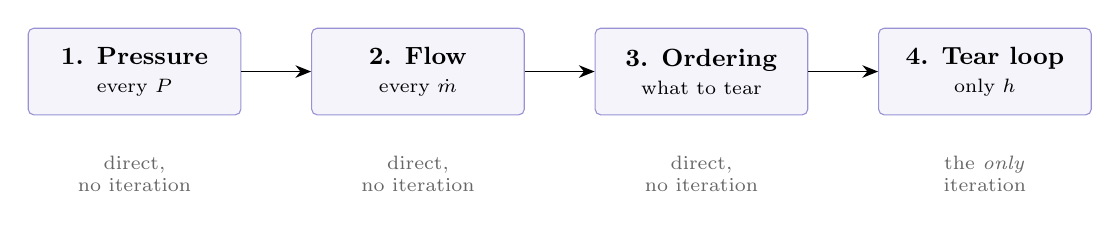
\begin{tikzpicture}[x=1cm,y=1cm,
  pass/.style={rectangle, rounded corners=2pt, draw=accent!60, fill=accent!6,
               minimum width=27mm, minimum height=11mm, font=\small, align=center}]
  \node[pass] (p1) at (0,0)   {\textbf{1. Pressure}\\[-1pt]\scriptsize every $P$};
  \node[pass] (p2) at (3.6,0) {\textbf{2. Flow}\\[-1pt]\scriptsize every $\dot m$};
  \node[pass] (p3) at (7.2,0) {\textbf{3. Ordering}\\[-1pt]\scriptsize what to tear};
  \node[pass] (p4) at (10.8,0){\textbf{4. Tear loop}\\[-1pt]\scriptsize only $h$};
  \draw[ar] (p1) -- (p2); \draw[ar] (p2) -- (p3); \draw[ar] (p3) -- (p4);
  \node[font=\scriptsize, text=black!60, align=center] at (0,-1.3)   {direct,\\no iteration};
  \node[font=\scriptsize, text=black!60, align=center] at (3.6,-1.3) {direct,\\no iteration};
  \node[font=\scriptsize, text=black!60, align=center] at (7.2,-1.3) {direct,\\no iteration};
  \node[font=\scriptsize, text=black!60, align=center] at (10.8,-1.3){the \emph{only}\\iteration};
\end{tikzpicture}
\caption{Four passes. The first three are bookkeeping and run once each. All
the real work, and all the possibility of not converging, is confined to the
fourth and to the smallest possible set of unknowns.}
\label{fig:passes}
\end{figure}

\section{Pass 1: pressures, which care about nothing else}

Here is the observation the whole design rests on.

Ask what sets the pressure at any point in the cycle. The compressor
discharge is whatever you specified. The turbine exhaust is whatever you
specified. A heat exchanger's outlet is its inlet minus a drop that depends
on the inlet pressure. A splitter hands the same pressure to both branches.

\emph{Not one of those answers mentions enthalpy.} The pressure field is
decoupled from the thermal problem entirely, so it can be solved first, by
itself, without a single property call.

\subsection{And it can be solved without iterating}

Every one of those relations is invertible. ``Outlet is inlet minus two
percent'' reads backwards just as easily as ``inlet is outlet divided by
\num{0.98}''. So a relation carries both directions:

\codefile[title={cycles/passes/pressure.py --- a two-way relation}]{relation.py}

\noindent Knowing both directions means the pass does not have to care which
pressures you happen to specify. Anchor the compressor inlet and it
propagates forwards to find the turbine exhaust. Anchor the turbine inlet
instead and the same relations run backwards to find the compressor
discharge. No branching, no special cases.

The pass then just sweeps the relation list, filling in whatever it can from
whatever it already knows, until a sweep changes nothing:

\codefile[title={cycles/passes/pressure.py --- the sweep}]{pressure_propagate.py}

\noindent It always terminates, because each sweep either learns something
or stops. If it stops with pressures still unknown, the case is
under-specified, and it is reported as that, by name, immediately. The
alternative would be for the missing pressure to surface much later as an
unexplained convergence failure.

\textbf{Partial cooling needed no new code here.} Three pressure levels
instead of two is not a special case for this pass. It is a different set of
anchors and relations, and the sweep handled it without being told anything
had changed.

\section{Pass 2: flows, for the same reason}

Mass flows decouple for the identical reason and the pass has the identical
shape. Each block states what it does to flow in one of three ways:

\codefile[title={cycles/blocks/base.py}]{flow_rules.py}

\noindent \code{Identity} means the outlet carries whatever came in:
compressors, turbines, heaters, coolers, and each side of an exchanger
separately. \code{Scale} is the splitter, handing fractions of its inlet to
its outlets. \code{Sum} is the mixer, running the other way.

Everything is a fraction of total cycle flow, so this pass is arithmetic
with no units in it. The absolute mass flow is not fixed until the end, once
the specific work and specific heat per kilogram are known and the plant's
size target can be divided by them. That ordering is deliberate: the entire
thermal solution is computed once and then scales to any plant size for
free.

\section{Pass 3: finding what is genuinely circular}

With pressures and flows known, only enthalpies remain, and the question
from the start of the chapter can finally be asked precisely: in what order
can the blocks be evaluated?

The rule is simply that a block can run once all its inlet streams are
known. So: find every block whose inlets are known, run it, mark its outlets
known, repeat.

Sooner or later this stalls. Blocks remain, but none of them has all its
inlets, and that is the loop making itself felt. The remedy is to
\textbf{tear}: pick one unknown stream, guess its enthalpy, and carry on as
though it were known. At the end of the sweep the network will have computed
a value for that same stream. If the computed value matches the guess, the
guess was right and the cycle is solved.

\subsection{Which stream to tear}

It matters, for a reason that is purely about cost. Every torn stream is one
more unknown in the iteration that follows, and the iteration is where all
the time goes. So the pass tears the stream that unblocks the most
downstream blocks, breaking ties towards the hot inlet of a heat exchanger,
which in a recuperator network is the physically natural choice since the
turbine will shortly be supplying it anyway.

\codefile[title={cycles/passes/ordering.py}]{ordering.py}

\begin{choicebox}
\textbf{A measurement changed this design.} The ordering pass originally
tore \emph{two} streams in the recompression layout.

The cause was that the heater had been left as an ordinary block, so the
solver had no way to know its outlet without first knowing its inlet, even
though the case specifies the turbine inlet temperature outright. Letting
the heater and cooler declare their outlets up front gives the ordering pass
one more known stream to start from, which is enough to collapse two tears
to one.

The answer is bit-for-bit identical. The runtime fell by a factor of
\num{33}.
\end{choicebox}

\section{Pass 4: the only iteration in the program}
\label{sec:tearloop}

One number remains, and one question: does guessing it reproduce it?

The method is \textbf{successive substitution}, which is as simple as it
sounds. Take what came out and use it as the next guess.

\subsection{Watching it converge}

Suppose the torn stream is the recuperator's hot inlet and its true enthalpy
is somewhere near \SI{557}{\kilo\joule\per\kilogram}, which nobody knows
yet. Start from a deliberately poor guess.

\begin{center}
\begin{tabular}{@{}rrrr@{}}
\toprule
Iteration & Guessed $h$ & Came back as & Gap \\
\midrule
1 & 500.0 & 540.0 & 40.0 \\
2 & 540.0 & 552.0 & 12.0 \\
3 & 552.0 & 555.6 &  3.6 \\
4 & 555.6 & 556.7 &  1.1 \\
5 & 556.7 & 557.0 &  0.3 \\
\bottomrule
\end{tabular}
\end{center}

Each gap is about \SI{30}{\percent} of the one before. The error is not
merely shrinking, it is shrinking by a constant factor every time, which
means a fixed number of iterations buys a fixed number of decimal places.
That behaviour has a name: the map is a \textbf{contraction}.

\codefile[title={cycles/passes/tear.py}]{tear_loop.py}

\subsection{Why it contracts}

Plain substitution looks too naive to work reliably, so it is worth knowing
why it does here rather than trusting that it will.

Follow a disturbance around the loop. Perturb the torn enthalpy and the
recuperator passes on only its effectiveness fraction of that perturbation,
because the rest goes into the other stream. The heater then erases
whatever reaches it, because it fixes an outlet temperature outright
regardless of what came in. The cooler does the same at the other end.

So a disturbance is attenuated several times per circuit and arrives back
much smaller than it left. That is exactly what a contraction is, and
contractions converge geometrically under plain substitution.

\begin{caveat}[title={Caveat: two attempts to speed this up both backfired}]
\textbf{Wegstein acceleration.} The textbook accelerator for successive
substitution extrapolates from the last two iterates. Applied here it
oscillated and stalled, never reaching tolerance. Adding the standard
safeguard restored convergence but took more than twice as many iterations
as doing nothing at all.

The diagnosis: Wegstein assumes a smooth, roughly linear map. This one is
neither, because the heat exchanger contains its own inner convergence
loop whose tolerance puts a small discontinuity into the outer map. The
code is gone and the reason is written into \code{passes/tear.py} so that
it does not get helpfully re-added.

\textbf{Loosening the inner tolerance.} The obvious alternative was to let
the exchanger's inner solve be sloppier, since the outer loop re-runs it
anyway. Relaxing it stopped the outer loop converging \emph{at all}: the
inner granularity became a noise floor that the outer residual could never
get below.

The fix was to keep the tight tolerance and reach it in fewer evaluations,
by warm-starting the inner search from the previous outer iterate. That cut
the slowest case by a factor of four with no loss of accuracy.

\textbf{The general lesson, which cost two days:} in nested iterations the
inner tolerance must be tighter than the outer one, and speed is bought with
better initial guesses, never with looser convergence.
\end{caveat}

\begin{caveat}[title={Caveat: contraction is a property of these cases, not a theorem}]
The argument above rests on the recuperator being lossy and on the heater
and cooler fixing their outlets. A layout that violates both, such as very
high effectiveness with no fixed outlet anywhere, could have a map that is
not a contraction, and plain substitution would then diverge.

\textbf{What to do if it happens:} \code{numerics.relax} below \num{1}
damps the update and is the first thing to try. If that fails the layout
needs a real Newton solve, which this program does not have. No case in this
project is near that boundary, but the boundary exists.
\end{caveat}

\section{What this bought}
\label{sec:explicit}

The simple recuperated layout needs \emph{no iteration at all}. With the
heater and cooler outlets declared, the ordering pass finds a sequence with
no circular dependency left, and the ``cycle'' solves in a single sweep. The
loop was never really a loop once the fixed temperatures were accounted for,
which is a satisfying result and not an obvious one.

Recompression and partial cooling each tear one stream and converge in under
thirty iterations. Specifying a pinch rather than an effectiveness costs
roughly an order of magnitude, because a specified pinch means searching for
the duty that produces it, so every outer iteration now contains an inner
search and every inner iterate is a full profile with two property calls per
node. That cost buys the ability to size exchangers the way the brief asks,
which is worth it. Timings are recorded with the saved results.

\section{What to remember}

\begin{itemize}\itemsep2pt
\item A cycle has no entry point: nothing can be computed first. That is
      what makes it hard.
\item Pressure and flow do not depend on enthalpy, so they can be solved
      first, directly, without iterating.
\item Pressure relations are invertible, so the pass works regardless of
      which pressures the user chose to specify.
\item What remains circular is torn: guess one enthalpy, sweep, check
      whether it came back.
\item Successive substitution converges because the loop attenuates
      disturbances. The error falls by a constant factor each pass.
\item Letting the heater declare its outlet collapsed two tears to one and
      cut the runtime by a factor of thirty.
\item In nested iterations, tighten the inner tolerance and buy speed with
      better guesses.
\end{itemize}

% =====================================================================
\chapter{The numerical methods}
\label{ch:numerics}

Chapter~\ref{ch:solving} described the \emph{architecture} of solving: four
passes, and one of them iterates. This chapter is about the arithmetic
inside that description --- which equations are solved by evaluation, which
need a search, what the searches actually do, how they decide they are
finished, and what happens when they are not.

The reason this deserves a chapter of its own is that a cycle solver is
easy to mistake for a collection of unrelated tricks. It is not. There are
only five kinds of problem in the whole program, and knowing which one you
are looking at tells you immediately what it costs and how it can fail.

\section{Five kinds of problem}
\label{sec:problemtypes}

Every calculation in the solver is one of these.

\begin{center}
\small
\begin{tabular}{@{}p{3.1cm}p{5.3cm}p{5.0cm}@{}}
\toprule
Kind & What it means & Where it happens \\
\midrule
\textbf{Direct evaluation} &
The unknown is on the left of an equals sign. Substitute and you are done. &
Turbine and compressor work, mixing, splitting, energy balances, pressure
drops \\[2pt]
\textbf{Property inversion} &
The equation of state is written in one set of variables and you have
another. A search, but somebody else's. &
Every $T(P,h)$, $h(P,s)$, $s(P,h)$ call --- inside CoolProp \\[2pt]
\textbf{Scalar root-find} &
One unknown, one equation, no closed form. Search a bracket. &
Heat-exchanger effectiveness for a pinch or a $UA$; coolant flow for a
pinch \\[2pt]
\textbf{Fixed point} &
$x = g(x)$, where $g$ means "go round the loop once". &
The tear stream in recompression and partial cooling \\[2pt]
\textbf{Scheduling} &
Not numerical at all: an ordering problem on a graph. &
Deciding which block to evaluate next, and what is genuinely circular \\
\bottomrule
\end{tabular}
\end{center}

Three things follow from that table, and they are the reason it is worth
drawing.

\textbf{The expensive kinds are rare.} Most of the program is the first row.
A recuperated cycle solves in one explicit pass with no search at all at
the cycle level (\S\ref{sec:explicit}) --- the only searches are inside the
exchanger and inside CoolProp.

\textbf{Property inversion is everywhere and invisible.} Every call to
$T(P,h)$ is a root-find that CoolProp performs, and there are hundreds of
thousands of them in a sweep. This is why the design decision of
Chapter~\ref{ch:props} --- carry $(P,h)$, never $(P,T)$ --- is a
\emph{numerical} decision as much as a thermodynamic one. Carrying the
wrong pair means paying for an inversion on every single state.

\textbf{Only one true fixed point exists in the program.} Everything else is
either direct or a bracketed scalar search. That is a deliberately small
numerical surface, and it is what makes the solver's failure modes few
enough to enumerate (\S\ref{sec:whenitfails}).

\section{Why everything is bracketed, and why Newton is absent}

A bracketed method is one that starts with an interval known to contain
the answer and never leaves it. Bisection is the archetype. Newton's
method is not bracketed: it follows the local slope and can land anywhere.

Newton is the obvious choice for a smooth scalar problem --- it converges
quadratically, roughly doubling the number of correct digits each step,
against bisection's one bit. It is not offered here, and the reason is
thermodynamic rather than numerical.

\begin{choicebox}[title={Why the pinch has a kink in it}]
Consider searching for the effectiveness that produces a given pinch.
Sweep effectiveness upward and the pinch falls. But \emph{where} the pinch
sits can move: at low effectiveness the closest approach is usually at one
end of the exchanger, and as effectiveness rises the profiles bend and the
closest approach migrates into the interior (\S\ref{sec:pinch}).

At the effectiveness where the minimum changes location, the pinch is
still continuous --- it does not jump --- but its \emph{slope} does. The
function has a kink.

A bracketed method does not notice. It only ever asks whether a value is
above or below the target. Newton asks for the derivative, and at a kink
there are two of them. Near that point Newton will overshoot, and because
it is unbracketed, nothing catches it.

So the choice is: give up quadratic convergence, or risk a method that
fails exactly at the configurations where the exchanger is most
interesting. That trade is why \code{cycles/numerics/roots.py} offers
bisection, a monotone wrapper around it, and a bracket-clamped secant ---
and no Newton.
\end{choicebox}

This is worth holding onto as a general lesson: \textbf{the smoothness of
a thermodynamic function is a physical question, not a mathematical
assumption you are free to make.}

\section{Bisection}

\textbf{The problem.} Find $x$ with $f(x) = 0$, knowing only that $f$
changes sign across $[lo, hi]$.

\textbf{The method.} Evaluate at the midpoint. The root is in whichever
half shows a sign change. Repeat.

\textbf{Why it is safe.} It assumes nothing but continuity and a sign
change. No derivative, no smoothness, no good initial guess. The bracket
can only shrink, so it cannot diverge.

\textbf{What it costs.} The interval halves every step, so the error falls
by a factor of two per iteration --- one bit at a time. Going from a
bracket of width 1 to an answer good to $10^{-10}$ takes about
$\log_2(10^{10}) \approx 34$ evaluations. Compare that with the handful
that a secant takes from a warm start, and you see why both exist.

\codefile[title={cycles/numerics/roots.py}]{bisect.py}

\textbf{The residual, and why the tolerance is relative.} The loop stops
when the bracket is narrower than
$\mathrm{tol} \times \max(1, |x|)$, not when it is narrower than
$\mathrm{tol}$. The $\max(1, |x|)$ makes the test relative for large
values and absolute for small ones. Without it the same tolerance would
mean wildly different things for an effectiveness near $0.9$ and an
enthalpy near $500\,000$: an absolute $10^{-10}$ on an enthalpy in joules
per kilogram is asking for sixteen significant figures, which double
precision cannot deliver, and the loop would run to its iteration cap
every time.

\textbf{When it fails.} Two ways, both raising \code{ConvergenceError}
with the numbers in the message: no sign change on the interval (the root
is not in there, or there is no root), or the iteration cap is reached.

\section{Monotone solving, and a decision about the impossible}

\code{solve\_monotone} answers a slightly different question: find $x$ with
$f(x) = \text{target}$, where $f$ is known to be monotone on the bracket.
Monotonicity is what guarantees there is exactly one answer, and here it is
a physical fact rather than an assumption --- both pinch and $UA$ move in
one direction as effectiveness rises.

Underneath it is bisection on $f(x) - \text{target}$. The interesting part
is what it does when the target cannot be reached at all.

\codefile[title={cycles/numerics/roots.py}]{solve_monotone.py}

\begin{choicebox}[title={Implementation: clamping is an engineering decision, not a numerical one}]
Ask for a \SI{5}{\kelvin} pinch from an exchanger whose profiles cannot
come closer than \SI{12}{\kelvin} and there is no answer. The honest
numerical response is to raise.

With \code{clamp=True} it instead returns the nearest endpoint, and the
caller flags the design. The reason is the sweep. A multi-objective run
evaluates dozens of candidates and a parametric study thousands; among
them there will always be some that ask for something impossible. One of
them raising would kill the whole run and lose every point computed before
it.

So the rule is: \textbf{an infeasible point must come back labelled, not
explode.} The same philosophy produces \code{Result(ok=False)} with a
reason rather than an exception at the top level, and it is why the
constraint filter in Chapter~\ref{ch:choosing} can report \emph{why} each
design was rejected instead of just that it was.

\code{clamp=False} is still there for a caller who wants the exception,
and nothing in this project uses it.
\end{choicebox}

\section{The secant method, warm-started}

\textbf{The problem.} The same scalar root-find --- but this time you
already have a very good guess, because you solved almost exactly this
problem one iteration ago.

That is the situation inside the tear loop. The exchanger is re-solved on
every pass while its hot inlet drifts slightly, so last pass's
effectiveness is nearly right. Throwing that away and bisecting from
scratch wastes about thirty evaluations per exchanger per iteration.

\textbf{The method.} Draw a straight line through the last two points and
take where it crosses the target:
\[
x_{n+1} = x_n - f(x_n)\,\frac{x_n - x_{n-1}}{f(x_n) - f(x_{n-1})}
\]
This is Newton with the derivative replaced by a finite difference of
values you already have --- so it needs no derivative and costs one
function evaluation per step. Its convergence is superlinear (order
$\approx 1.618$): not quite Newton, far better than bisection.

\codefile[title={cycles/numerics/roots.py}]{secant.py}

\textbf{The two safeguards matter more than the method.} The secant is
unbracketed, which is exactly what was ruled out above. It is used anyway,
under conditions that remove the risk:

\begin{enumerate}\itemsep2pt
\item \textbf{Every iterate is clamped into $[lo, hi]$}, and an iterate
      that lands outside breaks the loop rather than being pursued.
\item \textbf{The fallback is bisection.} If the secant stalls (a zero
      denominator, two iterates with the same value) or leaves the
      bracket, the function does not fail --- it hands the problem to
      \code{solve\_monotone} and the answer comes back a little slower.
\end{enumerate}

So the worst case is bisection's cost, and the usual case is three or four
evaluations. A fast method with a safe fallback is a different proposition
from a fast method alone, and the difference is the whole reason this is
acceptable where plain Newton was not.

\section{Which method goes where}

\begin{center}
\small
\begin{tabular}{@{}p{4.6cm}p{3.4cm}p{5.2cm}@{}}
\toprule
Calculation & Method & Why that one \\
\midrule
HX effectiveness, first pass &
\code{solve\_monotone} &
No previous answer to start from \\[2pt]
HX effectiveness, later passes &
\code{secant} (warm) &
Last pass's answer is nearly right \\[2pt]
Coolant flow for a pinch spec &
\code{solve\_monotone} &
Called once per solve; no warm start available \\[2pt]
The tear stream &
\code{successive\_substitution} &
The map is contractive; see \S\ref{sec:tearloop} \\[2pt]
Everything else &
direct evaluation &
No search needed \\
\bottomrule
\end{tabular}
\end{center}

\codefile[title={cycles/blocks/heat\_exchanger.py}]{hx_seek.py}

Three lines, and they are the warm-start decision in full: bisect when
there is nothing to start from, secant when there is.

\section{The fixed point, and its initial guess}

The tear loop itself --- successive substitution, why it contracts, and
the Wegstein acceleration that backfired --- is in \S\ref{sec:tearloop}
and is not repeated here. Two things belong in this chapter instead.

\textbf{The residual.} What the loop actually tests is
\[
r = \max_{s \,\in\, \text{tears}}
    \frac{|g(x_s) - x_s|}{\max(|x_s|,\,|g(x_s)|,\,1)}
\]
--- a \emph{relative} change, maximised over all torn streams, for the
same reason bisection's tolerance is relative. With a single tear and
enthalpies around \SI{500}{\kilo\joule\per\kilogram}, the default
$\mathrm{tol} = 10^{-8}$ means the guess and what came back agree to about
eight significant figures, which is $5\times10^{-6}$~\si{\joule\per\kilogram}:
far below anything physically meaningful, and cheap because the map
contracts geometrically.

\textbf{The initial guess is domain-informed, and has to be.}

\codefile[title={cycles/solve.py}]{tear_guess.py}

A quarter of the way up the cycle's temperature span, converted to an
enthalpy at the stream's known pressure. The comment in the source gives
the reason in one line: successive substitution is forgiving, but a guess
in the wrong phase region is not. Start a \ce{CO2} tear stream below the
saturation dome and the first pass computes properties for a liquid that
the converged cycle never contains; the iteration may then wander, or
converge onto something unphysical. The guess does not need to be good. It
needs to be in the right region.

\section{Two loops, one inside the other}
\label{sec:twoloops}

This is the subtlest numerical point in the program and the one most worth
understanding.

The tear loop is the outer iteration. Inside each of its passes, every
heat exchanger runs its own search for effectiveness. So there is a loop
inside a loop, and their tolerances are not independent.

\begin{center}
\begin{tabular}{@{}llr@{}}
\toprule
Loop & Where & Tolerance \\
\midrule
Outer: tear stream & \code{Numerics.tol} & $10^{-8}$ (relative) \\
Inner: HX effectiveness & \code{\_seek(..., tol)} & $10^{-9}$ \\
Inner: coolant flow & \code{coolant.size} & $10^{-6}$ \\
Property inversion & CoolProp internal & $\sim 10^{-12}$ \\
Energy closure check & \code{Numerics.energy\_tol} & $10^{-3}$ (diagnostic) \\
\bottomrule
\end{tabular}
\end{center}

\textbf{The inner tolerance must be tighter than the outer one, and the
reason is not fussiness.} The outer loop measures how much the torn
enthalpy changed from one pass to the next. If the exchanger inside only
resolves its own answer to $10^{-6}$, then feeding it the identical input
twice can return answers differing by $10^{-6}$ --- and the outer loop
cannot tell that apparent change from a real one. Its residual then has a
floor it can never get below, and it iterates to the cap and fails, with
every individual component apparently working correctly.

That is a genuinely nasty failure: nothing is wrong, and the solver says
it did not converge. The fix is an ordering, not a number --- the inner
tolerance is one decade tighter than the outer, so inner noise sits below
the outer convergence test.

\begin{caveat}
This interaction is also the reason Wegstein acceleration failed here
(\S\ref{sec:tearloop}). Wegstein extrapolates, which assumes the map is
smooth. The inner loop's finite tolerance puts a small discontinuity into
the outer map, the extrapolation reads it as signal, and the iteration
oscillates. The failure of a textbook accelerator was diagnostic of a real
structural feature, not a bug.

The coolant tolerance is loose ($10^{-6}$) because coolant sizing happens
\emph{once}, after the cycle has converged. It is outside both loops, so
it cannot pollute either.
\end{caveat}

\section{When it fails}
\label{sec:whenitfails}

Every failure in the numerical layer raises \code{ConvergenceError}, and
every one of them is caught in exactly one place.

\begin{center}
\small
\begin{tabular}{@{}p{4.3cm}p{4.0cm}p{4.6cm}@{}}
\toprule
Failure & Raised by & What the user sees \\
\midrule
No sign change on the bracket & \code{bisect} &
flag naming the interval and both end values \\[2pt]
Iteration cap hit & \code{bisect}, \code{successive\_substitution} &
flag with the final residual \\[2pt]
Target physically unreachable & \code{solve\_monotone} (\code{clamp=False}) &
flag naming the achievable range \\[2pt]
Tear will not settle & \code{passes/tear.py} &
flag naming the streams, residual, and the suggestion to lower
\code{relax} \\
\bottomrule
\end{tabular}
\end{center}

\code{solve()} wraps the whole tear in a \code{try}, and a
\code{ConvergenceError} becomes \code{Result(ok=False)} carrying the
message as a flag. A second, broader \code{except} does the same for
anything else.

\textbf{So a failed point is data.} It does not raise, it does not print,
and it does not stop a sweep --- it comes back as a \code{Result} whose
\code{ok} is false and whose \code{flags} say why. The multi-objective run
in Chapter~\ref{ch:choosing} relies on this completely: of its candidates,
the ones that fail to solve are simply absent from the comparison and the
ones that solve but break a constraint are present and labelled. Neither
case costs the other candidates anything.

\begin{caveat}[title={Caveat: silence is the risk this creates}]
The price of never crashing is that a failure can go unnoticed. A sweep
that silently drops a third of its points still prints a tidy table.

Two habits guard against it, and they are habits rather than code: every
run script reports how many candidates solved out of how many were tried,
and \code{Result.summary()} prints flags whenever there are any. If a
number of candidates comes back lower than the grid you asked for, that is
the signal to look --- the solver will not raise it for you.
\end{caveat}

\section{Where the tolerances come from}

Honestly: three of the five are conventional choices that turned out to be
comfortably adequate, and saying so is better than inventing a derivation.

\begin{itemize}\itemsep3pt
\item $10^{-8}$ on the tear is about half of double precision's
      significant digits, which leaves ample headroom above round-off
      while being reached in five or six passes because the map contracts
      by roughly a factor of three each time (\S\ref{sec:tearloop}).
\item $10^{-9}$ on the exchanger is \emph{derived}: one decade below the
      outer loop, for the reason in \S\ref{sec:twoloops}. This one is not
      arbitrary.
\item $10^{-6}$ on coolant flow is loose on purpose --- it is outside both
      loops, and it sizes a cooler to six figures, which is five more than
      the \SI{2.5}{\kilo\gram\per\kilo\watt\per\kelvin} mass conversion
      deserves.
\item $10^{-3}$ on energy closure is not a solver tolerance at all. It is
      a \emph{diagnostic} threshold: a check that the first law holds
      across the converged cycle. Observed closure is around
      $2\times10^{-14}$, so the gate is eleven orders of magnitude looser
      than what the solver actually achieves, which is the right way round
      for a check that should fire only when something is genuinely broken.
\end{itemize}

\begin{caveat}[title={Not yet verified}]
What is \emph{not} established is that the engineering conclusions are
insensitive to these choices. The argument above says each tolerance is
far below physical significance, which is persuasive but not evidence.
A sweep that re-runs the recommended design across a decade of each
tolerance and reports the spread in $\eta_{th}$ would settle it, and is
listed in Chapter~\ref{ch:open} as outstanding.
\end{caveat}

\section{What to remember}

\begin{itemize}\itemsep2pt
\item There are five kinds of problem in the solver, and only one of them
      --- the tear --- is a genuine fixed point. Most of the program is
      direct evaluation.
\item Property inversion is the hidden cost. Carrying $(P,h)$ instead of
      $(P,T)$ is a numerical decision as much as a thermodynamic one.
\item Everything is bracketed because the pinch function has a kink where
      the closest approach migrates into the interior. Smoothness is a
      physical question, not a free assumption.
\item Bisection costs one bit per evaluation and assumes almost nothing.
      The warm-started secant costs three or four evaluations and falls
      back to bisection when it misbehaves.
\item Tolerances are relative, not absolute, or the same number means
      different things for an effectiveness and an enthalpy.
\item The inner loop's tolerance must be tighter than the outer's, or
      inner noise puts a floor under the outer residual and a perfectly
      healthy cycle reports non-convergence.
\item A failure is data: \code{Result(ok=False)} with a reason, never an
      exception. The cost is that silence must be watched for.
\end{itemize}

% =====================================================================
\chapter{From a solved cycle to a plant}
\label{ch:sizing}

\section{Scaling}

The solver works per kilogram. Turning that into a plant is one division.

Efficiency is dimensionless and comes out of the per-kilogram solution
unchanged. Everything else scales linearly. Suppose the solve gives a
specific heat input $q_{in} = \SI{250}{\kilo\joule\per\kilogram}$ and a net
specific work $w_{net} = \SI{120}{\kilo\joule\per\kilogram}$. For the
brief's \SI{100}{\mega\watt} reactor:
\[
  \dot m = \frac{\dot Q}{q_{in}}
         = \frac{100 \times 10^3}{250}
         = \SI{400}{\kilogram\per\second},
  \qquad
  W_{net} = \dot m\, w_{net}
          = 400 \times 120 = \SI{48}{\mega\watt}.
\]
Every other power and conductance follows the same way.

\codefile[title={cycles/solve.py (excerpt)}]{metrics.py}

\noindent The sums are by block \emph{kind}, not by name. That is why
recompression needed no special-casing: its second compressor has
\code{kind == "compressor"}, so it is in the sum, and nothing had to be told
it existed.

\section{What the four numbers are worth}
\label{sec:metrics}

Four quantities come out, and they differ sharply in how much weight they
can carry. Knowing which is which matters more than knowing their values.

\textbf{Thermal efficiency} $\eta_{th} = W_{net}/Q_{in}$ is the solid one.
Two quantities the solver computes directly from first-law balances,
verified against a closed form to machine precision
(Appendix~\ref{app:validation}). Trustworthy to the digits reported.

\textbf{Back-work ratio} $W_c/W_t$ is equally solid and more diagnostic than
it looks. It is the single number saying how much of the cycle's advantage
survived. Chapter~\ref{ch:work} introduced it as the reason sCO$_2$ is
interesting at all; watching it climb when recompression is switched on is
watching that advantage being partly spent.

\textbf{Total conductance} $\sum UA$ is where the program stops doing
thermodynamics and starts making claims about hardware, and it should be
read with more suspicion than the first two. The $UA$ values themselves are
computed correctly from the profiles. What is \emph{not} established is the
step from conductance to size, which needs a heat transfer coefficient $U$
this program never computes. Reporting $\sum UA$ as a size \emph{proxy} is
defensible, because for one exchanger technology size does scale with it.
Reporting it as a size is not.

\textbf{Heat rejection ratio} $Q_{out}/W_{net}$ is the cooling burden per
unit of output, and it is what connects the cycle to a site. A value near
\num{1.7} means the plant must dump \SI{70}{\percent} more heat than it
produces electricity, which is what the tonne-per-second of cooling water in
Chapter~\ref{ch:precooler} is for.

\begin{caveat}[title={Caveat: this is thermal efficiency, not plant efficiency}]
$\eta_{th}$ counts shaft work. The brief asks about a power plant, and the
gap is not small: generator and gearbox losses, cooling-water pumping, and
the reactor's own auxiliaries all sit between the turbine shaft and the
grid.

\textbf{What it costs:} a net plant efficiency a few points below the
$\eta_{th}$ reported here is the honest expectation. Quoting $\eta_{th}$ as
though it were plant efficiency is the easiest available way to overstate
the result.
\end{caveat}

% =====================================================================
\chapter{Exergy: where the losses actually are}
\label{ch:exergy}

\section{What the first law cannot tell you}

Chapter~\ref{ch:sizing} ended with four numbers, and all four share a
blind spot.

Thermal efficiency says a cycle turns \SI{36.5}{\percent} of its heat into
work. It does not say \emph{where the other \SI{63.5}{\percent} went}, and
it cannot, because energy is conserved. Every joule that enters leaves
again, so a first-law balance can account for all of it and still be silent
about which component wasted it. Two cycles with identical efficiency can
have completely different problems.

That is the gap this chapter fills. The question is not where the energy
went --- it went into the river --- but where the \emph{ability to do work}
went, which is a different quantity and is not conserved.

\section{Exergy, and the entropy tax}

The exergy of a stream is the work you could extract from it, at best, by
bringing it reversibly into equilibrium with the surrounding environment.
Once it has reached that environment it can do nothing more, so its exergy
is zero by construction. That end point is the \textbf{dead state}.

For a flowing stream, physical flow exergy is
\begin{equation}
  e_x = (h - h_0) - T_0 (s - s_0)
  \label{eq:exergy}
\end{equation}
where subscript 0 is the dead state. Read it as two terms that fight.

The first, $h - h_0$, is the energy the stream carries above the
environment. If that were all, exergy and energy would be the same thing
and this chapter would be pointless.

The second is the price. A stream that carries entropy cannot have all its
energy converted: some must be dumped as heat at environment temperature,
and $T_0(s - s_0)$ is exactly how much. Call it the entropy tax.

\subsection{Put numbers through it}

Suppose a stream sits \SI{600}{\kilo\joule\per\kilogram} above the dead
state in enthalpy, and \SI{0.40}{\kilo\joule\per\kilogram\per\kelvin} above
it in entropy, with the environment at \SI{300}{\kelvin}:
\[
  e_x = 600 - 300 \times 0.40 = 600 - 120
      = \SI{480}{\kilo\joule\per\kilogram}.
\]
Of \SI{600}{\kilo\joule\per\kilogram} of energy, \SI{480}{} is in principle
available as work and \SI{120}{} is not, and nothing you build can recover
that \SI{120}{}. The second law took it before you started.

\subsection{Why it is destroyed rather than lost}

Now the part that makes exergy useful. Energy is conserved; exergy is not.
Every irreversible process destroys some, and the amount is
\[
  \dot E_D = T_0 \dot S_{\text{gen}},
\]
the Gouy--Stodola result. Entropy generated anywhere, at any temperature,
costs work potential in proportion.

So a component's exergy destruction is a direct measure of how much damage
its irreversibility does, in kilowatts, comparable across components that
have nothing else in common. A compressor's friction and a heat exchanger's
temperature difference are not otherwise commensurable; in exergy they are.

\section{The reference environment}

Exergy is always relative to something, so the dead state is an input, not
a constant. The defaults are \SI{298.15}{\kelvin} and
\SI{101325}{\pascal}: ambient, one atmosphere.

\codefile[title={cycles/physics/exergy.py}]{exergy_specific.py}

\begin{choicebox}
It is a field on the \code{Case}, like everything else a run fixes, so a
sensitivity study on ambient temperature is \code{case.with\_(environment=
Environment(T0=degC(40)))} and not an edit to the source.

\code{dead\_state} is cached because it depends only on the fluid and the
environment, so it is identical for every stream in a case. Without the
cache it cost two property lookups per exergy evaluated, which was most of
this module's property traffic for no information.
\end{choicebox}

\begin{caveat}[title={Caveat: physical exergy only, and that is correct here}]
Equation~\eqref{eq:exergy} is \emph{physical} flow exergy. A full accounting
adds a chemical term for the work available from bringing the stream's
composition to equilibrium with the environment.

It is omitted, and for once that is not an approximation. The working fluid
is \ce{CO2} everywhere and its composition never changes, so the chemical
term is identical at every point in the cycle and cancels exactly from every
difference taken. Kinetic and potential terms are dropped for the same
reasons they are dropped from the energy balances.
\end{caveat}

\section{Destruction, component by component}

Every block gets the same balance. In general, for a steady component,
\[
  \dot E_D = \sum_{\text{in}} \dot m e_x
           - \sum_{\text{out}} \dot m e_x
           + \sum_j \left(1 - \frac{T_0}{T_{b,j}}\right)\dot Q_j
           - \dot W_{\text{out}},
\]
with heat into the component positive and shaft work out of it positive.

For most of the blocks here it collapses to something far simpler, and the
reason is worth seeing. If a component is adiabatic --- no heat crosses its
boundary --- the $\dot Q$ term vanishes, and then the enthalpy and work
terms cancel against each other by the energy balance the solver has
already satisfied. What is left is pure entropy:
\[
  \dot E_D = T_0 \sum \dot m \,\Delta s .
\]

That is true for the compressors, the turbine, the throttle, both
recuperators, the mixer and the splitter: everything except the heater and
the coolers. So one entropy sum over a block's own streams does all of
them.

\codefile[title={cycles/physics/exergy.py}]{exergy_balance.py}

\begin{choicebox}
The solver already computed a per-block entropy balance, as a second-law
sign check. This module extends that same balance to the remaining block
types rather than writing a parallel implementation, which is why adding
exergy changed no existing number: it reads the same entropy field the
checks were already built on.
\end{choicebox}

\subsection{Worked, on a compressor and a recuperator}

Take a plant flowing \SI{400}{\kilogram\per\second} with the environment at
\SI{300}{\kelvin}.

\paragraph{Compressor.} An ideal one is isentropic, so
$\Delta s = 0$ and it destroys nothing, however much work it absorbs.
Give the real one an entropy rise of
\SI{0.006}{\kilo\joule\per\kilogram\per\kelvin}:
\[
  \dot E_D = 400 \times 300 \times 0.006 = \SI{720}{\kilo\watt}.
\]

\paragraph{Recuperator.} Both streams count, and they pull opposite ways.
The hot side cools, so its entropy falls, say by
\SI{0.50}{\kilo\joule\per\kilogram\per\kelvin}; the cold side warms, so its
entropy rises, say by \SI{0.60}{}. At equal flows the sum is
$+\SI{0.10}{}$, and
\[
  \dot E_D = 400 \times 300 \times 0.10 = \SI{12}{\mega\watt}.
\]
Sixteen times the compressor, from a component with no moving parts. That
is not a mistake, and \S\ref{sec:exresults} is about why.

\paragraph{Splitter and mixer.} A splitter sends the same state two ways and
generates nothing. A mixer joins streams at different states, which is
irreversible, and its destruction is the entropy that mixing creates.

\label{sec:nosource}
\section{The two components that cannot be done, and the one rule that fixes it}

Exergy destruction needs the temperature at which heat crosses the boundary,
because that is what sets how much exergy the heat carries. For two blocks,
this project does not know it.

\paragraph{The heater has no heat source.} Chapter~\ref{ch:machines} said
this plainly: the block is told an outlet temperature and reports a duty.
There is no reactor behind it, no primary loop, no boundary temperature.
The heat arrives from nowhere at an unknown temperature.

The tempting move is to use the \ce{CO2} outlet temperature as the boundary.
That is wrong and badly so: heat only flows down a temperature difference,
so the source must be hotter, and the whole irreversibility of the heater
lives in precisely that gap. Assuming it away reports zero destruction for
the component that may well have the most.

\paragraph{The coolers depend on what you specified.} Give a cooler a
coolant side (Chapter~\ref{ch:precooler}) and the coolant's inlet and outlet
states are known, so the \ce{CO2} and the coolant together form an adiabatic
pair and the balance closes honestly. Give it none and the rejection
temperature is unknown, exactly like the heater.

\begin{choicebox}
\textbf{The same rule as the pressure drops in \S\ref{sec:pumping}: the
solver uses a boundary temperature you state, and never invents one.}

With no \code{T\_source} on the heater, its destruction is reported as
\emph{unavailable}, with the reason, and the total is labelled incomplete.
State one and it becomes computable. Either way the program does not guess,
and the distinction between ``not computed'' and ``computed as zero'' is
never blurred.
\end{choicebox}

\noindent It is worth stating a source temperature once, just to see the
size of what is being left out. On the baseline, with the reactor side
assumed at \SI{650}{\celsius}:

\begin{center}
\begin{tabular}{@{}lrr@{}}
\toprule
Stated $T_{\text{source}}$ & Heater $\dot E_D$ [\si{\mega\watt}]
  & Total [\si{\mega\watt}] \\
\midrule
none                & unavailable & incomplete (\num{20.07} known) \\
\SI{550}{\celsius}  &  9.88 & 29.96 \\
\SI{650}{\celsius}  & 13.80 & 33.88 \\
\bottomrule
\end{tabular}
\end{center}

At \SI{650}{\celsius} the heater destroys more than the recuperator does
--- it would be \emph{the largest single irreversibility in the plant}. So
the component the model cannot compute is quite possibly the worst one, and
quietly reporting zero for it would have inverted the conclusion of
\S\ref{sec:exresults}. This is the clearest case in the project of why an
unavailable number must be labelled unavailable rather than defaulted.

Note also how strongly it moves with the assumption: \SI{100}{\kelvin} of
source temperature is \SI{4}{\mega\watt} of destruction. That sensitivity is
the reason the figure is not quietly adopted as a default.

\section{Closing the books}

An exergy balance that does not close is worthless, so there has to be a
check. The difficulty is that a balance drawn around the whole plant
\emph{cannot} close here, because the exergy entering with the reactor heat
is exactly the unknown above.

The way out is to move the boundary. Draw it at the \ce{CO2} side of the
heater instead of around the reactor, and every term becomes something the
solver computed:
\[
  \underbrace{\Delta \dot E_{x,\text{heater}}}_{\text{exergy the \ce{CO2} gains}}
  = \underbrace{\dot W_{\text{net}}}_{\text{work out}}
  + \underbrace{\dot E_{D}}_{\text{destroyed}}
  + \underbrace{\dot E_{x,\text{coolant}}}_{\text{carried away}}
\]

On the baseline, in megawatts: $55 = 37 + 17 + 1$.

The last term is the one that catches people. Warm cooling water still has
work potential relative to the environment; it is \emph{shed}, not
destroyed. Treating it as destruction double-counts, and treating it as zero
leaves the balance open. The computed residual is around
\num{4e-8} of the exergy supplied, which is the check passing.

\begin{caveat}[title={Caveat: negative destruction is never clipped}]
A negative exergy destruction is a second-law violation and therefore a bug:
a sign error, a bad converged state, or a modelling mistake. Taking absolute
values or flooring at zero would hide exactly the thing worth finding.

Anything materially negative is flagged. The threshold scales with the
largest destruction in the cycle, so it tracks genuine floating-point noise
rather than a fixed number that means different things in different cases.
\end{caveat}

\section{What the numbers say}
\label{sec:exresults}

For the recompression cycle at a \SI{5}{\kelvin} pinch:

\begin{center}
\small
\begin{tabular}{@{}llrr@{}}
\toprule
Block & Kind & $\dot E_D$ [\si{\mega\watt}] & Share [\si{\percent}] \\
\midrule
HTR & heat\_exchanger & 6.09 & 45.3 \\
TURB & turbine & 2.90 & 21.6 \\
PC & cooler & 1.82 & 13.5 \\
LTR & heat\_exchanger & 0.90 & 6.7 \\
MC & compressor & 0.70 & 5.2 \\
RC & compressor & 0.64 & 4.8 \\
MIX & mixer & 0.40 & 3.0 \\
SPLIT & splitter & 0.00 & 0.0 \\
HEATER & heater & --- & --- \\
\bottomrule
\end{tabular}

\end{center}
\from{exergy/by_component.csv}{python -m project.studies.exergy}

\textbf{The recuperator is the largest irreversibility, in every
layout} --- \SIrange{45}{76}{\percent} of the accounted total depending
on configuration. That is the capacity-rate mismatch of
Chapter~\ref{ch:recup} seen a second way. Heat crossing a finite
temperature difference destroys availability, and the mismatch is
exactly what forces that difference to stay open along most of the
exchanger.

This is worth dwelling on, because it is the payoff of doing a
second-law analysis at all. The first law told us the recuperator
needed to be large. The second law tells us \emph{why} it has to be
large: not because there is a lot of heat to move, but because the heat
is being moved badly, across a gap that the fluid's own properties hold
open. Two analyses, one mechanism.

\textbf{The turbine is second at \SI{21.6}{\percent}}, which is
unavoidable --- that is what a \num{0.90} isentropic efficiency costs
in availability. \textbf{The compressors together destroy
\SI{1.34}{\mega\watt}}, about a fifth of the recuperator's figure,
which is the back-work-ratio story again: cheap compression is also
clean compression.

\begin{caveat}[title={The total is incomplete, and must say so}]
The heater's destruction cannot be computed: the model takes the
reactor as given and has no heat-source boundary temperature, so the
entropy generated pushing heat into the cycle is unknown. The entry is
blank with a stated reason, never zero, and every total above is a
partial sum.

It is not a small omission. With a plausible \SI{650}{\celsius} source
the heater would destroy about \SI{13.8}{\mega\watt} --- more than the
recuperator, and the largest single irreversibility in the cycle. The
layouts stay comparable because the same term is missing from each, but
no absolute figure here is a complete accounting.
\end{caveat}

The complete per-layout tables, and what they imply for the design
choice, are in the final report.

\section{What this is for, and what it is not}

Exergy is a diagnostic here. It is deliberately not an optimisation
objective, and the metrics of Chapter~\ref{ch:sizing} are unchanged: nothing
in this chapter moved a single first-law number.

The reason is that minimising exergy destruction is not the same as
maximising efficiency or minimising cost, and assuming otherwise is a known
trap. You could drive recuperator destruction towards zero by making the
exchanger infinitely large, which is thermodynamically splendid and
commercially absurd. Destruction tells you \emph{where} to spend; it does
not tell you \emph{whether} spending is worth it.

Read the three metrics together:

\begin{center}
\begin{tabular}{@{}lp{0.62\linewidth}@{}}
\toprule
$\eta_{th}$ & how well the cycle does overall \\
$\sum UA$ & what hardware that costs \\
$\dot E_D$ by component & \emph{which} component is responsible, and so
  where more hardware would actually buy something \\
\bottomrule
\end{tabular}
\end{center}

\begin{caveat}[title={Caveat: the total is incomplete and should be labelled so}]
Every total in this chapter excludes the heater. Reporting it as total cycle
exergy destruction would be wrong, and the code refuses to: the total is
\code{None} unless every component is accounted for, with
\code{E\_D\_known} reported separately and \code{exergy\_complete} saying
which it is.

\textbf{What it costs:} the layout \emph{comparison} is sound, because every
layout is missing the same term and their heaters do similar work.
A statement about the absolute irreversibility of the plant is not available.
\end{caveat}

\section{Running it}

\begin{quote}\small
\code{python -m project.runs.exergy} \quad component breakdown, all layouts,
plus a sweep over the split fraction\\
\code{python -m project.runs.validate\_exergy} \quad the 16 checks\\
\code{python -m project.runs.compare\_layouts} \quad efficiency, $UA$ and
destruction side by side
\end{quote}

\noindent From Python, \code{result.exergy} holds everything:
per-component \code{E\_D}, \code{fractions}, \code{by\_kind},
per-stream \code{e\_x}, the balance residual, and \code{incomplete} listing
what could not be computed and why. \code{result.state\_table()} now carries
a specific-exergy column.

\section{What to remember}

\begin{itemize}\itemsep2pt
\item Energy is conserved, so efficiency cannot say \emph{where} a cycle
      loses. Exergy is not conserved, so it can.
\item $e_x = (h-h_0) - T_0(s-s_0)$: energy above ambient, minus the entropy
      tax on it.
\item For an adiabatic component everything cancels except
      $\dot E_D = T_0 \sum \dot m\,\Delta s$.
\item An ideal machine destroys nothing however much work it moves; only
      irreversibility costs.
\item The heater cannot be computed because the project has no heat source.
      State a \code{T\_source} and it can. The solver never invents one.
\item Close the books at the \ce{CO2} side of the heater, and remember that
      warm coolant is exergy \emph{shed}, not destroyed.
\item The recuperator is the biggest irreversibility in every layout, and it
      is the capacity-rate mismatch seen a second way.
\item Exergy says where to spend, not whether to. It is a diagnostic, not an
      objective.
\end{itemize}

% =====================================================================
\chapter{Choosing one design}
\label{ch:choosing}

Everything up to here has computed. This chapter decides, which is a
different kind of operation and a weaker one, and most of the work is in
being honest about how much weaker.

\section{Why ``optimise the cycle'' is not yet a question}

Ask a solver to maximise efficiency and it will answer. Ask it to maximise
efficiency \emph{and} minimise mass and it has nothing to answer with,
because the two instructions point in opposite directions and no arithmetic
reconciles them. This is not a shortcoming of the solver. It is a property
of the question.

Here is the smallest version of the problem. Suppose two designs:

\begin{center}
\begin{tabular}{lcc}
\toprule
 & efficiency & mass \\
\midrule
design A & \SI{40}{\percent} & \SI{100}{\tonne} \\
design B & \SI{38}{\percent} & \SI{70}{\tonne} \\
\bottomrule
\end{tabular}
\end{center}

Which is better? The question has no answer. It has an answer once somebody
says how much a tonne is worth in efficiency points, and that somebody is
not the thermodynamics. A reactor on a barge and a reactor on a prepared
site will give different answers to the same pair of designs, using the same
physics.

So the honest output of a multi-objective problem is not a design. It is
three things, in order:

\begin{enumerate}\itemsep2pt
\item the designs that are \emph{allowed} --- the constraint filter;
\item of those, the ones nothing else beats outright --- the frontier;
\item and then, separately and visibly, a \emph{choice}.
\end{enumerate}

Steps 1 and 2 are computation and the program does them. Step 3 is a
judgement, and the most useful thing the program can do there is make its
own judgement easy to overrule.

\section{Four objectives, and what stands in for each}

The brief names four things to optimise. None of them can be measured
directly from a solved cycle, so each needs a proxy, and every proxy is a
modelling decision that deserves to be visible.

\textbf{Efficiency} is the one honest objective. $\eta_{th} = w_{net}/q_{in}$
comes straight out of the solver (\S\ref{sec:metrics}) with no proxy at all.

\textbf{Mass and volume} are what compactness means, and here the brief
hands over a single conversion: a printed-circuit exchanger weighs about
\SI{2.5}{\kilo\gram} per \si{\kilo\watt\per\kelvin} of $UA$. That is the
whole bridge from thermodynamics to hardware, and it is why
Chapter~\ref{ch:recup} spent so long on $UA$: the conductance was never an
academic quantity, it is the mass of the plant in different units.

The arithmetic is then trivial, which is exactly why the reading underneath
it matters. Take a recuperator that the solver sizes at
\SI{4000}{\kilo\watt\per\kelvin}. At \SI{2.5}{\kilo\gram} per unit that is
\SI{10}{\tonne} of exchanger. The brief independently assumes a
\SI{10}{\tonne} baseline recuperator, so the conversion and the solver agree
without having been made to --- a small validation that costs nothing and is
worth noticing.

\begin{caveat}[title={Caveat: two readings the brief does not settle}]
\textbf{The precooler.} The brief gives the \SI{2.5}{\kilo\gram} figure for
the recuperator and says only that the precooler ``scales with heat rejected
per \si{\mega\watt}$_e$''. Both are printed-circuit exchangers doing the
same job in the same technology, so the same conversion is applied to the
precooler's $UA$. That is a reading, not a quotation, and it is consequential:
the precooler is the \emph{larger} exchanger
(\S\ref{sec:everysink}), so it carries more mass than the recuperator in
every layout. Anyone who disagrees with the reading should expect the
mass ranking to move.

\textbf{Volume.} There is a baseline volume (\SI{120}{\cubic\metre}) and a
baseline mass (\SI{60}{\tonne}) but no volume-per-$UA$. Their ratio,
\SI{0.5}{\tonne\per\cubic\metre}, is used as a density throughout. This
means volume carries \emph{no information that mass does not}, and a
\si{\mega\watt}$_e$ per \si{\cubic\metre} figure is the mass figure
rescaled. It is reported because the brief asks for it, not because it is
independent evidence.
\end{caveat}

\textbf{The cost proxy} is hardware at about US\$250 per kilogram
against electricity at about US\$70 per \si{\mega\watt\hour} for
some \SI{7000}{\hour} a year. The brief calls this a proxy and it is right
to: there is no fuel, no O\&M, no financing, no discounting, no civil works.
The absolute dollars mean very little.

What a proxy this crude \emph{is} good for is one specific comparison, and
it happens to be the one the project asks: does the extra hardware of a
better layout earn its keep against the extra electricity it makes? Put
round numbers through it. Suppose a layout adds \SI{20}{\tonne} and
\SI{4}{\mega\watt}$_e$. The hardware is $20\,000 \times 250 = \text{US\$5M}$. The electricity is $4 \times 70 \times 7000 = \text{US\$1.96M}$ a year. It pays for itself in about two and a half
years, against a plant that will run for decades. That conclusion survives
being wrong about the price of steel by a factor of two, which is the only
reason it is worth stating at all.

\begin{caveat}
Payback needs no plant lifetime; an annualised cost does, because a one-off
hardware bill and a yearly energy income cannot be added without one. The
code therefore reports both, with the lifetime named as a constant
(\num{30} years) rather than buried in a formula --- but payback is the more
honest of the two, and it is what the brief's own worked example computes.
\end{caveat}

\textbf{Operational margin} is distance from the two-phase region at the
compressor inlet, in \si{\kelvin} above the critical temperature and
\si{\mega\pascal} above the critical pressure. It is the only objective that
is not about money or efficiency, and it exists because the whole cycle is
deliberately parked next to a cliff (Chapter~\ref{ch:props}). A design that
is one kelvin from the dome is not a design, it is a dare.

\begin{choicebox}[title={Implementation: which inlet}]
Margin has to be measured at every \emph{compressor} inlet, not at the
coldest stream in the cycle. The distinction is invisible in recompression,
where the coldest stream \emph{is} the main-compressor inlet, and decisive in
partial cooling, where the coldest stream feeds a pre-compressor at an
intermediate pressure while the main compressor sits somewhere else entirely.
Measuring at the coldest stream gave partial cooling inconsistent verdicts
until the measurement was moved.

\codefile[title={project/assessment/metrics.py}]{inlets.py}

The function walks the layout for blocks that compress, takes each one's
inlet stream, and returns the minima. Nothing about \ce{CO2} or about this
project's five layouts appears in it; it asks the layout what its
compressors are.
\end{choicebox}

\section{The specific-power trap}

There is a fifth number that looks like an objective and is not:
\si{\mega\watt}$_e$ per \si{\tonne}, electrical output over plant mass. It is
the obvious compactness figure and the brief asks for it.

It is also almost pure arithmetic. Efficiency and mass are already two of the
four objectives; their ratio adds no information, and it is \emph{biased}:
because mass is dominated by exchangers and exchanger mass grows faster than
efficiency does, specific power is maximised by the \emph{least} efficient
design on the frontier. Optimise it alone and you will build the plain
recuperated cycle every time.

So it is reported alongside the objectives and never used as one. A derived
ratio in an objective list is a double count wearing a disguise.

\section{The filter, and the one limit that is ambiguous}

Constraints come first and they are cheap: they throw designs away without
any argument about priorities. The brief gives six.

\begin{center}
\begin{tabular}{ll}
\toprule
limit & why it exists \\
\midrule
compressor inlet $\ge \SI{32}{\celsius}$ & clear of the two-phase region \\
compressor inlet $\ge \SI{7.7}{\mega\pascal}$ & same \\
recuperator pinch $\ge \SI{5}{\kelvin}$ & finite exchanger
(\S\ref{sec:pinch}) \\
cycle pressure $\le \SI{20}{\mega\pascal}$ & vessels and seals \\
turbine inlet $\le \SI{500}{\celsius}$ & materials \\
split fraction $\le 0.5$ & more than half is a different cycle \\
\bottomrule
\end{tabular}
\end{center}

Five of these are unambiguous. The sixth is not, and it changes the answer.

``Compressor inlet $\ge \SI{32}{\celsius}$ and $\ge \SI{7.7}{\mega\pascal}$
(safe distance from the two-phase region)'' admits two readings:

\begin{itemize}\itemsep2pt
\item \textbf{Literal.} Every compressor inlet meets both numbers.
\item \textbf{By intent.} Every compressor inlet is a safe distance from the
      two-phase region --- which, above the critical temperature, it is at
      \emph{any} pressure, because there is no dome up there to be near.
\end{itemize}

Partial cooling is exactly the case that separates them. Its pre-compressor
inlet sits at an intermediate pressure of about \SI{6}{\mega\pascal} ---
below the stated limit --- at \SI{32}{\celsius}, which is above the critical
temperature and therefore nowhere near a phase boundary. The literal reading
rejects the entire partial-cooling family. The reading by intent admits all
of it.

\begin{caveat}[title={Caveat: this one is unresolved}]
The default is the literal reading, because a number in a brief is a number.
A single flag switches it, and the run prints how many designs the choice
admits or rejects. It is not a detail to be smoothed over: with the literal
reading the partial-cooling family never reaches the frontier, and the
recommendation below is a recompression cycle partly \emph{because} of a
reading of a parenthesis. This belongs in a conversation with whoever wrote
the brief, not in a footnote.
\end{caveat}

\begin{choicebox}[title={Implementation: the filter returns its rejects}]
\codefile[title={project/assessment/moo.py}]{feasible.py}

The function returns \emph{every} design tagged, not only the survivors.
That is deliberate twice over. The brief asks for ``the feasible set after
constraint filtering'' as a deliverable, and the value of such a deliverable
is mostly in what was excluded and why --- a filter whose rejects are
invisible cannot be checked. And each violation carries its own sentence
with the measured number in it, so a rejection reads as
\code{compressor inlet 6.00 MPa < 7.7 MPa} rather than \code{False}.

The tolerance exists so that a design sitting exactly on a limit is
admitted. Floating-point arithmetic will otherwise reject a pinch of
\num{5.0} kelvin about half the time, which is the kind of bug that produces
a confident wrong answer rather than a crash.
\end{choicebox}

\section{Dominance: discarding what nobody would choose}

After filtering there are still dozens of designs and still no way to rank
them. But some of them can be discarded \emph{without} anyone stating a
priority, and that is the one piece of free progress available.

Four designs, invented and round:

\begin{center}
\begin{tabular}{lccl}
\toprule
 & efficiency & mass & \\
\midrule
A & \SI{40}{\percent} & \SI{100}{\tonne} & \\
B & \SI{38}{\percent} & \SI{70}{\tonne} & \\
C & \SI{36}{\percent} & \SI{90}{\tonne} & worse than B on \emph{both} \\
D & \SI{40}{\percent} & \SI{110}{\tonne} & same as A, heavier \\
\bottomrule
\end{tabular}
\end{center}

C and D can go. Not because efficiency matters more than mass or less, but
because whatever your priorities, B is better than C and A is better than D.
Nobody with any set of weights would choose them. C is \textbf{dominated} by
B, and D by A.

A and B survive. Neither dominates the other: A is better on efficiency, B
on mass, and choosing between them requires a priority that the data does
not contain. What survives is therefore precisely the set where priorities
begin to matter --- and the point of computing it is that it is the last
thing computable before judgement has to enter.

\begin{choicebox}
\codefile[title={project/assessment/moo.py}]{dominance.py}

\code{\_dominates(a, b)} is the definition read straight off: at least as
good everywhere, strictly better somewhere. Minimised objectives are negated
so one comparison handles both senses, which avoids the branching that makes
this kind of function quietly wrong in one direction.

\code{pareto\_front} is then the brute-force $O(n^2)$ sweep, deliberately.
There are clever algorithms for this; there are also \num{43} designs here,
and the loop runs in microseconds. Spending complexity on it would buy
nothing and cost a reader's afternoon.
\end{choicebox}

\section{Picking a point, and admitting it is a pick}

The frontier does not choose. Two standard rules will:

\textbf{Weighted sum.} Pick weights, add the normalised objectives, take the
best. Honest in that the weights are visible; dishonest in that somebody had
to invent four numbers, and the result is extremely sensitive to them.

\textbf{Knee point.} Normalise each objective onto $[0,1]$ across the
frontier, construct the corner where every objective simultaneously takes
its best value --- a point no real design reaches, since if one did the
frontier would be a single dot --- and take whichever design sits closest to
that ideal.

The knee is used here, and it is worth being precise about what it assumes:
equal weighting of all four objectives, which nobody asked for. It is not
neutral merely because no weights were typed. What it is good for is as a
\emph{starting point for an argument}: it lands somewhere defensible, and
shifting the weights moves the pick along the frontier in a way anyone can
inspect.

\begin{choicebox}
\codefile[title={project/assessment/moo.py}]{knee.py}

The normalisation is per-objective and across the front only, so an
objective that barely varies cannot dominate the distance by accident of
units. Efficiency in percent and mass in tonnes would otherwise be compared
as raw numbers, and mass would win every time for no reason but arithmetic.
The guard on a zero range keeps a degenerate front (every design identical
on one objective) from dividing by zero.
\end{choicebox}

\section{What the sweep found}

The decision variables swept are the ones the brief names: maximum pressure,
split fraction, compressor-inlet temperature, and layout. Every combination
is solved, assessed, filtered, and plotted.

\subsection{Pressure}

\begin{figure}[htbp]
\centering
\begin{tikzpicture}
\begin{axis}[width=12cm, height=5.6cm,
  xlabel={Maximum cycle pressure [\si{\mega\pascal}]},
  ylabel={$\eta_{th}$ [\si{\percent}]},
  xmin=13.6, xmax=20.4, ymin=29, ymax=44,
  legend pos=south east, legend style={font=\small,draw=black!30},
  grid=both, grid style={black!8},
  tick label style={font=\small}, label style={font=\small}]
\addplot[accent, thick, mark=*, mark size=1.4pt]
  table[x=P_high,y=eta_recup] {data/eta_vs_rp.dat};
\addlegendentry{recuperated}
\addplot[warn, thick, mark=square*, mark size=1.4pt]
  table[x=P_high,y=eta_recomp] {data/eta_vs_rp.dat};
\addlegendentry{recompression}
\end{axis}
\end{tikzpicture}
\caption{Efficiency against maximum pressure, at a fixed
\SI{7.7}{\mega\pascal} compressor inlet, so the horizontal axis is also the
pressure ratio ($r_p$ from \num{1.82} to \num{2.60}). Both curves rise
monotonically and both are still rising at the right-hand edge: the optimum
is the constraint, not an interior maximum. The vertical gap between the
curves is what the split buys, and it does not close.}
\label{fig:eta_rp}
\end{figure}

Both curves climb all the way to the limit and flatten as they go. This is
worth pausing on, because it is the opposite of what the textbook
air-standard Brayton cycle does.

In the ideal air cycle, efficiency depends on pressure ratio alone and rises
without bound; in a \emph{real} one with a fixed turbine inlet temperature
there is an interior optimum, because past some ratio the compressor eats
work faster than the turbine gains it. Here the back-work ratio is around
\num{0.2} rather than \num{0.5} (\S\ref{sec:bwr}), so compression is cheap
enough that the crossover has not happened by \SI{20}{\mega\pascal}. The
limit arrives first.

That makes the pressure decision easy and uninteresting: go to the
constraint. It also means the \SI{20}{\mega\pascal} ceiling is doing real
work in this project. Raise it and the answer moves.

\subsection{Split fraction}

\begin{figure}[htbp]
\centering
\begin{tikzpicture}
\begin{axis}[width=12cm, height=5.6cm,
  xlabel={Split fraction $x$ (fraction bypassing the precooler)},
  ylabel={$\eta_{th}$ [\si{\percent}]},
  xmin=0.07, xmax=0.48, ymin=36.5, ymax=45.5,
  legend pos=north west, legend style={font=\small,draw=black!30},
  grid=both, grid style={black!8},
  tick label style={font=\small}, label style={font=\small}]
\addplot[warn, thick, mark=square*, mark size=1.4pt]
  table[x=x,y=eta_recomp] {data/eta_vs_x.dat};
\addlegendentry{recompression}
\addplot[accent, thick, mark=*, mark size=1.4pt]
  table[x=x,y=eta_partial] {data/eta_vs_x.dat};
\addlegendentry{partial cooling}
\end{axis}
\end{tikzpicture}
\caption{Efficiency against split fraction at \SI{20}{\mega\pascal}.
Recompression has a genuine interior optimum near $x = 0.40$ and falls away
beyond it. Partial cooling is still climbing at $x = 0.45$, and is lower
everywhere in this range --- consistent with Dostal's finding that it wins
below about \SI{20}{\mega\pascal} only in its improved-regeneration form
(\S\ref{sec:dostal}), which is not what is modelled here.}
\label{fig:eta_x}
\end{figure}

This is the opposite shape, and the reason is the whole argument of
Chapter~\ref{ch:splitting} seen from the outside. Sending more fluid round
the recompressor relieves the capacity-rate mismatch in the low-temperature
recuperator, which is pure gain --- until too little fluid is left going
through the precooler to absorb the heat that has to leave. Then the
recuperator starts starving and the curve turns over. An interior optimum is
the signature of two effects of opposite sign, and here you can name both.

\subsection{The frontier}

\begin{figure}[htbp]
\centering
\begin{tikzpicture}
\begin{axis}[width=12.5cm, height=7cm,
  xlabel={PCS mass [\si{\tonne}]},
  ylabel={$\eta_{th}$ [\si{\percent}]},
  xmin=64, xmax=108, ymin=31, ymax=44.5,
  legend pos=south east, legend style={font=\small,draw=black!30},
  grid=both, grid style={black!8},
  tick label style={font=\small}, label style={font=\small}]
\addplot[only marks, mark=x, mark size=2.6pt, black!25]
  table[x=mass,y=eta] {data/pareto_dominated.dat};
\addlegendentry{dominated}
\addplot[only marks, mark=o, mark size=2.4pt, warn!70]
  table[x=mass,y=eta] {data/pareto_infeasible.dat};
\addlegendentry{infeasible}
\addplot[only marks, mark=*, mark size=2.6pt, accent]
  table[x=mass,y=eta] {data/pareto_front.dat};
\addlegendentry{frontier}
\addplot[only marks, mark=star, mark size=4.5pt, chalk, thick]
  table[x=mass,y=eta] {data/pareto_knee.dat};
\addlegendentry{knee}
\end{axis}
\end{tikzpicture}
\caption{Efficiency against mass for all \num{43} designs. The frontier runs
up and to the right: every efficiency point costs tonnes, and nothing in the
cloud escapes that. Note where the infeasible designs sit --- several are
\emph{above} the frontier, which is the constraint filter doing its job
rather than a plotting error. The highest-efficiency design in the whole
sweep is infeasible. Note also that a few dominated crosses sit above and
left of a frontier point: dominance is judged on all four objectives at
once, and a design that looks better in this projection is losing on cost or
on margin. Any two-dimensional view of a four-dimensional frontier will do
that.}
\label{fig:pareto_mass}
\end{figure}

Two features of Figure~\ref{fig:pareto_mass} carry the argument.

\textbf{The frontier is short.} Of \num{36} feasible designs, five are
non-dominated. Thirty-one were beaten outright by something else, no
priorities required. That is the free progress of the previous section,
cashed in.

\textbf{Some of the best designs are not allowed.} The infeasible markers
include the most efficient design found anywhere in the sweep. One is
rejected for a pinch of \num{4.98} kelvin against a \num{5.00} limit, which
is close enough to be worth saying out loud: it is not a bad design, it is a
design whose exchanger is slightly too small, and \num{0.02} kelvin of
specification is the only thing standing between it and the frontier. The
other six are the partial-cooling family, rejected by the reading of the
inlet-pressure limit discussed above.

\begin{figure}[htbp]
\centering
\begin{tikzpicture}
\begin{axis}[width=12.5cm, height=6.4cm,
  xlabel={$\eta_{th}$ [\si{\percent}]},
  ylabel={Specific power [MW$_e$ per tonne]},
  xmin=31, xmax=44.5, ymin=0.37, ymax=0.57,
  legend pos=north east, legend style={font=\small,draw=black!30},
  grid=both, grid style={black!8},
  tick label style={font=\small}, label style={font=\small}]
\addplot[only marks, mark=x, mark size=2.6pt, black!25]
  table[x=eta,y=mwe_per_t] {data/pareto_dominated.dat};
\addlegendentry{dominated}
\addplot[only marks, mark=o, mark size=2.4pt, warn!70]
  table[x=eta,y=mwe_per_t] {data/pareto_infeasible.dat};
\addlegendentry{infeasible}
\addplot[only marks, mark=*, mark size=2.6pt, accent]
  table[x=eta,y=mwe_per_t] {data/pareto_front.dat};
\addlegendentry{frontier}
\addplot[only marks, mark=star, mark size=4.5pt, chalk, thick]
  table[x=eta,y=mwe_per_t] {data/pareto_knee.dat};
\addlegendentry{knee}
\end{axis}
\end{tikzpicture}
\caption{The same designs, plotted as specific power against efficiency, and
the reason specific power is not used as an objective. The frontier slopes
\emph{down}: the most compact design per megawatt is the least efficient one
on it. Maximise this ratio and you select the plain recuperated cycle, every
time, by construction rather than by engineering.}
\label{fig:pareto_power}
\end{figure}

Figure~\ref{fig:pareto_power} is the specific-power trap drawn. The frontier in
Figure~\ref{fig:pareto_mass} slopes up; the same frontier in
Figure~\ref{fig:pareto_power} slopes down. Both are true, and a reader shown
only the second would conclude that the simplest layout is the best one.

\section{The recommendation}

\begin{center}
\begin{tabular}{ll}
\toprule
\multicolumn{2}{l}{\textbf{Recompression, \SI{20}{\mega\pascal},
$x = 0.25$, \SI{35}{\celsius} compressor inlet}} \\
\midrule
thermal efficiency & \SI{41.41}{\percent} \\
second-law efficiency & \num{0.684} \\
PCS mass & \SI{87.0}{\tonne} \\
specific power & \num{0.476}\,\si{\mega\watt}$_e$/\si{\tonne} \\
inlet margin & \SI{4.02}{\kelvin}, \SI{0.32}{\mega\pascal} \\
recuperator pinch & \SI{5.00}{\kelvin} \\
payback vs.\ best feasible recuperated & \num{2.3} years \\
\bottomrule
\end{tabular}
\end{center}

Four things about it are worth more than the numbers.

\textbf{It is not the most efficient design on the frontier.} Two
recompression designs beat it, by up to \num{1.4} points, and both are
heavier. The knee gives up those points for roughly \SI{17}{\tonne}.

\textbf{It is not the most compact either.} The plain recuperated cycle at
\SI{68.5}{\tonne} is lighter and has the best specific power on the
frontier. It is also four efficiency points worse, and the extra hardware
that closes that gap pays for itself in a little over two years against a
plant meant to run for thirty.

\textbf{The compressor inlet is at \SI{35}{\celsius}, not at the
constraint.} This is the least obvious part of the recommendation and the
most interesting. The brief's floor is \SI{32}{\celsius} and that is where
the \SI{7.7}{\mega\pascal} pressure makes the fluid densest, so running
there should make compression cheapest --- and it does, by a lot. Moving the
inlet from \num{32} to \SI{35}{\celsius} makes compression roughly
\SI{60}{\percent} more expensive per kilogram.

And the efficiency goes \emph{up}.

The reason is the subject of Chapter~\ref{ch:splitting}. A warmer, less
dense compressor inlet produces a warmer recuperator cold inlet, which eases
the capacity-rate mismatch, which lets the recuperator recover more heat,
which means the reactor has to supply appreciably less. Compression got more
expensive and the heat bill fell by more. The cycle does not care which of
its terms improved.

It also buys the margin: \SI{1.0}{\kelvin} at the constraint becomes
\SI{4.0}{\kelvin} at \SI{35}{\celsius}. A design that is better on
efficiency \emph{and} better on safety margin, at the cost of some exchanger,
is the rare case where two objectives stop disagreeing --- and it would have
been missed entirely by anyone who assumed the optimum sits at the critical
point because that is where the density is.

\textbf{It is a knee point, which is a rule and not a result.} Equal
weighting of four objectives is a judgement. Weight efficiency harder and
the pick slides up the frontier to the \SI{18}{\mega\pascal}
$x = 0.35$ design; weight mass harder and it slides down to the recuperated
cycle. The frontier is the finding. The point on it is a recommendation.

\subsection{The cycle itself}

\begin{figure}[htbp]
\centering
\begin{tikzpicture}
\begin{axis}[width=12.5cm, height=8.4cm,
  xlabel={Specific entropy [\si{\kilo\joule\per\kilogram\per\kelvin}]},
  ylabel={Temperature [\si{\celsius}]},
  xmin=1.54, xmax=2.80, ymin=0, ymax=560,
  legend pos=south east, legend style={font=\small,draw=black!30},
  grid=both, grid style={black!8},
  nodes near coords, point meta=explicit symbolic,
  every node near coord/.append style={font=\scriptsize, anchor=south east,
                                       inner sep=1.5pt, black!75},
  tick label style={font=\small}, label style={font=\small}]
\addplot[accent, thick, mark=*, mark size=1.5pt]
  table[x=s,y=T,meta=name] {data/ts_path.dat};
\addlegendentry{main loop}
\addplot[warn, thick, dashed, mark=square*, mark size=1.5pt]
  table[x=s,y=T,meta=name] {data/ts_branch.dat};
\addlegendentry{recompression branch}
\end{axis}
\end{tikzpicture}
\caption{The recommended cycle in the $T$--$s$ plane, every state numbered.
$1 \to 2$ is the main compressor, nearly vertical because compressing a
dense fluid costs little entropy; $2 \to 3 \to 4 \to 5$ is the two
recuperators and the mixing point, climbing the left-hand side at constant
pressure; $5 \to 6$ is the reactor; $6 \to 7$ is the turbine, dropping
temperature at almost constant entropy; $7 \to 8 \to 9$ is the same two
recuperators handing the heat back, and the long bottom leg $9 \to 1$ is the
precooler. The dashed branch is the quarter of the flow that skips the
precooler: it is compressed from state~9 straight to state~10 and rejoins at
state~4.}
\label{fig:ts}
\end{figure}

Two things are visible there that no table shows.

\textbf{The loop is thin.} The two recuperator legs --- cold side going up,
hot side coming down --- run close together over most of their length. That
narrow gap is the pinch, the capacity-rate mismatch, and the
largest single irreversibility in the cycle (Chapter~\ref{ch:exergy}), all
being the same thing seen in temperature--entropy coordinates.

\textbf{The precooler leg is short.} Almost all the heat that leaves the hot
stream is handed to the cold stream rather than to the water. That is the
recuperator earning its \SI{10}{\tonne}, and it is why this cycle works at
all.

\section{What would overturn this}

A recommendation worth anything says what would change it.

\begin{itemize}\itemsep3pt
\item \textbf{The inlet-pressure reading.} Admit the partial-cooling family
      and six designs re-enter the comparison, several of them competitive.
      This is the single largest open item and it is a question about English,
      not about thermodynamics (\S\ref{sec:choosing}).
\item \textbf{The \SI{20}{\mega\pascal} ceiling.} Figure~\ref{fig:eta_rp}
      shows both layouts still climbing at the limit. Raise it and every
      number here moves; the ranking probably does not, but the optimum
      pressure certainly does.
\item \textbf{The precooler mass reading.} Apply a different conversion to
      the precooler's $UA$ and the mass axis rescales non-uniformly across
      layouts, because recompression deliberately shrinks the precooler
      (\S\ref{sec:totalua}). That is the reading most likely to move the
      frontier.
\item \textbf{Turbomachinery mass.} Held constant across layouts, which
      understates the recompressor's real footprint beyond the brief's
      \SI{1.5}{\tonne} and ignores turbine size changing with flow.
      Chapter~\ref{ch:notmodelled} lists what else is absent.
\item \textbf{The weights.} Not a modelling error, a stated choice. It moves
      the pick along the frontier and nothing else.
\end{itemize}

\chapter{Two kinds of input}
\label{ch:inputs}

\section{A distinction borrowed from somewhere it was clearer}

The same distinction turned up in the Joule--Thomson cryocooler project and
was easier to see there, so it is worth transplanting.

Some inputs are \textbf{boundary conditions}. The environment hands them to
you and no amount of design changes them. Others are \textbf{design
variables}. You choose them, and choosing well is the engineering.

\begin{center}
\begin{tabular}{@{}lll@{}}
\toprule
& \textbf{Boundary conditions} & \textbf{Design variables} \\
\midrule
set by & reactor, site, materials & the designer \\
\midrule
 & reactor duty, \SI{100}{\mega\watt_{th}}   & pressure ratio \\
 & turbine inlet, \SI{500}{\celsius}         & split fraction $x$ \\
 & compressor inlet, \SI{32}{\celsius}       & recuperator $\varepsilon$ or pinch \\
 & max pressure, \SI{20}{\mega\pascal}       & layout \\
 & min compressor inlet, \SI{7.7}{\mega\pascal} & number of stages \\
 & machine efficiencies                      & low-pressure level \\
\bottomrule
\end{tabular}
\end{center}

The distinction is operational rather than philosophical: \textbf{sweep the
design variables, hold the boundary conditions fixed}. An optimisation that
improves efficiency by raising the turbine inlet temperature has not
optimised the cycle, it has changed the problem and answered a different
one.

\section{What a case looks like}

\codefile[title={project/cases/pdf\_baseline.py}]{case_baseline.py}

\noindent A case is a frozen dataclass. Plain Python, so an editor completes
the field names and a typo is an error at import rather than a wrong number
in a results table two hours later.

It is also the \emph{only} place where \ce{CO2}, \SI{20}{\mega\pascal} and
\SI{500}{\celsius} appear anywhere in the project. The solver does not know
them, the blocks do not know them, the layouts do not know them.

Variants come from \code{with\_()}, which deep-merges into a copy and leaves
the original untouched:

\begin{quote}\small
\code{pdf\_baseline\_dp = pdf\_baseline.with\_(params=\{"RECUP": \{"dP\_hot": 0.02\}\})}
\end{quote}

\noindent so the pressure-drop variant cannot silently drift away from the
baseline it is meant to be compared against.

\begin{caveat}[title={Caveat: YAML was considered and rejected}]
A configuration file would separate ``data'' from ``code'', which sounds
tidy. In practice it means inventing syntax for things Python already has:
references between fields, unit conversions, derived values, variants of a
base case. Then writing a parser for that syntax, and error messages for the
parser. Every one of those is somewhere the configuration can be wrong in a
way that surfaces as a confusing runtime failure far from its cause.

A frozen dataclass gives the same declarative feel with the editor, the type
checker and the import-time error all working for free.

\textbf{What it costs:} a case is a Python file, so someone who does not
write Python cannot author one. Acceptable here, not universally.
\end{caveat}

% =====================================================================
\chapter{Why none of this mentions \ce{CO2}}
\label{ch:generality}

\section{The separation}

Nothing in \code{cycles/} knows what fluid it is working with, what the
cycle is for, or even that it is a Brayton cycle. It knows that streams have
a pressure, an enthalpy and a flow, that blocks transform streams, and that
some property backend can answer questions about a fluid named by a string.

\begin{center}
\begin{tabular}{@{}p{0.45\linewidth}p{0.45\linewidth}@{}}
\toprule
\textbf{\code{cycles/} --- the solver} & \textbf{\code{project/} --- this project} \\
\midrule
streams, blocks, passes, physics,
property backends, numerics &
layouts, cases, runs, figures \\[2pt]
knows \emph{how} to solve a flowsheet &
knows \emph{which} flowsheet, and with what numbers \\[2pt]
contains no \ce{CO2}, no \SI{20}{\mega\pascal},
no Brayton &
contains nothing about solving \\
\bottomrule
\end{tabular}
\end{center}

\section{What it bought}

This is not an abstract virtue. Three things came free.

\textbf{A Rankine cycle is the same program.} From the solver's point of
view the only difference is that one of them crosses a saturation dome. The
state variables are still $(P,h)$. The compressor becomes a pump and is
still $\int v\,\mathrm{d}P$. The heater becomes a boiler and is still ``fix
the outlet temperature''. The condenser is the cooler. The saturation guard
in Chapter~\ref{ch:recup} was written precisely so the two-phase region does
not break this, and it was tested on water at \SI{10}{\kilo\pascal} for
exactly that reason. No block needs changing.

\textbf{Air validation required only a backend.} Checking the solver against
the closed-form ideal-gas Brayton result needed an ideal-gas property
backend, about a hundred lines, and \emph{nothing else}. No block, pass or
physics function was touched, because none of them had assumed a real fluid
in the first place.

\textbf{Partial cooling cost zero solver code.} Eleven blocks, fourteen
streams, three pressure levels, one layout file.

\begin{caveat}[title={Caveat: generality tested three times is a hypothesis}]
Three uses is encouraging and it is not proof. The abstraction is known to
hold for Brayton variants and for an ideal gas. The Rankine claim above is
reasoned rather than run.

\textbf{The honest statement:} no leak has been found yet, which is a
different thing from there being none.
\end{caveat}

% =====================================================================
\chapter{The studies, one by one}
\label{ch:studies}

A study is a question put to the solver. This chapter documents each of
the nine, to the same twelve points, so that running one does not
require reading its source.

The governing rule, which Chapter~\ref{ch:reproduce} then turns into
commands: \textbf{a study computes once and saves; everything
downstream reads the saved file.} Figures, tables and the report never
re-solve. That is not tidiness --- it is the only thing that stops a
figure and a recommendation describing different designs, which has
happened here once already.

\section{What every study has}

\begin{center}
\small
\begin{tabular}{@{}p{3.2cm}p{10.4cm}@{}}
\toprule
An entry point & a module under \code{project/studies/}, run with
\code{python -m}. Nothing imports it. \\
A saved result & one or more CSVs under \code{results/<study>/}. \\
A manifest & \code{manifest.json}: purpose, script, command, the grids
actually swept, environment, and a \textbf{source fingerprint} --- a
SHA-256 over every \code{.py} in \code{cycles/}, \code{brayton\_cycle/}
and \code{project/}. Two runs agreeing on that hash ran identical code,
uncommitted edits included. \\
Printed output & a human summary. It is a convenience, never the
record. \\
\bottomrule
\end{tabular}
\end{center}

\begin{caveat}
A manifest records a \emph{source} fingerprint rather than a commit
hash. There is no repository history for this work, and inventing a
commit identifier would be worse than having none. When one exists, the
commit belongs \emph{alongside} the fingerprint, not instead of it: the
fingerprint also catches edits that were never committed, which is
precisely the state in which most results get produced.
\end{caveat}

\section{Run order}

Only two dependencies exist, and both are checked at run time with an
error that names the command to run first.

\begin{center}
\begin{tabular}{@{}lll@{}}
\toprule
Study & Needs & Because \\
\midrule
\code{selected\_design} & \code{tradeoff} & it reads the knee row \\
\code{tolerances} & \code{tradeoff} & same \\
\code{make\_figures}, \code{make\_tables} & all studies & they read
saved results \\
\bottomrule
\end{tabular}
\end{center}

Everything else is independent and may be run in any order.

\section{Layout comparison}

\textbf{Question.} At equal thermodynamic quality of heat exchange ---
a common \SI{5}{\kelvin} pinch --- how do the four configurations
compare on efficiency, and what does each cost in exchanger?

\textbf{Theory.} Chapters \ref{ch:recup} and \ref{ch:splitting}. The
comparison must be on \emph{total} conductance, recuperators and
coolers together (\S\ref{sec:totalua}); counting recuperators alone
reverses the ranking.

\textbf{Fixed.} \SI{100}{\mega\watt} thermal, \SI{500}{\celsius}
turbine inlet, water-cooled, \SI{5}{\kelvin} recuperator pinch.
\textbf{Swept.} Layout only.

\textbf{Entry point.} \code{project/studies/compare\_layouts.py}, via
\code{cycles.solve} and \code{project.assessment}.
\textbf{Command.} \code{python -m project.studies.compare\_layouts}.
\textbf{Output.} \code{results/layout\_comparison/layouts.csv}.
\textbf{Figures.} None directly; feeds the report's comparison table.

\textbf{Verification.} Every row is a converged solve with its energy
closure checked. \textbf{Limitations.} Partial cooling's exhaust
pressure is held at its own swept optimum; see below.

\section{Parameter sweeps}

\textbf{Question.} How does efficiency vary with maximum pressure, and
with the recompression split fraction?

\textbf{Theory.} \S\ref{sec:bwr} for why the pressure curve does not
turn over where an air-standard cycle's would; Chapter~\ref{ch:splitting}
for why the split curve has an interior optimum.

\textbf{Fixed.} \SI{7.7}{\mega\pascal} compressor inlet,
\SI{5}{\kelvin} pinch. \textbf{Swept.} Maximum pressure
\SIrange{14}{20}{\mega\pascal}; split \numrange{0.10}{0.45}.

\textbf{Entry point.} \code{project/studies/sweeps.py}.
\textbf{Command.} \code{python -m project.studies.sweeps}.
\textbf{Output.} \code{results/parameter\_sweeps/pressure\_sweep.csv},
\code{split\_fraction\_sweep.csv}.
\textbf{Figures.} Both $\eta$ curves in the report.

\begin{caveat}
These grids are deliberately \emph{finer} than the trade-off study's.
That is not an inconsistency: a sweep exists to show the shape of a
curve and wants many points, while the trade-off evaluates full
candidate designs and wants few. Both record their own grid in their own
manifest. Before this study existed, the two sweeps were computed
separately on different grids inside the plotting script --- they agreed
only because both happened to call the same solver, and nothing enforced
it.
\end{caveat}

\section{Partial cooling's exhaust pressure}

\textbf{Question.} Partial cooling has a third pressure level that the
brief does not pin down. Where should it sit, and does choosing it well
change the layout ranking?

\textbf{Theory.} Lowering the exhaust widens the expansion and gains
turbine work, but the fluid must then be compressed from a lower and
less dense state. Two effects of opposite sign imply an interior
optimum. A third effect is specific to this layout: the pre-compressor
outlet feeds the low-temperature recuperator, so the exhaust pressure
also moves the capacity-rate mismatch.

\textbf{Swept.} Exhaust \SIrange{5.0}{7.6}{\mega\pascal}; then split
\numrange{0.20}{0.40} at the best exhaust pressure.

\textbf{Entry point.} \code{project/studies/partial\_cooling.py}.
\textbf{Command.} \code{python -m project.studies.partial\_cooling}.
\textbf{Output.} \code{results/partial\_cooling/}.

\textbf{Verification.} Two of the swept pressures do not solve, and the
reason is physical rather than numerical: as the exhaust approaches the
main compressor inlet, the pre-compressor has almost no work to do, the
second precooler's duty collapses and its coolant profile crosses. The
study records the failure and its reason rather than dropping the point.

\textbf{Limitations.} The sweep is one-dimensional at a time, not a
joint optimisation over exhaust pressure and split together.

\section{Intercooling's intermediate pressure}

\textbf{Question.} The companion to the above. Where should the
intermediate pressure sit, and does intercooling pay at all?

\textbf{Theory.} \S\ref{sec:intercooling}: cheaper compression against
recuperable heat thrown away. The ideal-gas geometric-mean rule is a
guess to be checked, not an answer.

\textbf{Swept.} Intermediate pressure \SIrange{7.9}{18}{\mega\pascal},
spanning the geometric mean. The lower end approaches the compressor
inlet, where the layout degenerates into the plain recuperated cycle ---
which is the limit against which intercooling must justify itself.

\textbf{Entry point.} \code{project/studies/intercooling.py}.
\textbf{Command.} \code{python -m project.studies.intercooling}.
\textbf{Output.} \code{results/intercooling/pressure\_sweep.csv}.

\section{Cooling}

\textbf{Question.} How much water does each cooler need, how large is
it, and what does moving the water cost?

\textbf{Theory.} Chapter~\ref{ch:precooler}. Four coolant specifications
collapse to one flow; the pinch sticks once water is plentiful, at the
\ce{CO2} outlet minus the water inlet.

\textbf{Entry point.} \code{project/studies/cooling.py}.
\textbf{Command.} \code{python -m project.studies.cooling}.
\textbf{Output.} \code{results/cooling/per\_cooler.csv},
\code{water\_sweep.csv}.

\textbf{Limitations.} Pressure drops are stated, never derived: this
project computes $UA$ and not geometry, so a geometry-based drop would
describe an exchanger unrelated to the one being sized.

\section{Exergy}

\textbf{Question.} Where is the available work actually destroyed?

\textbf{Theory.} Chapter~\ref{ch:exergy}.
\textbf{Entry point.} \code{project/studies/exergy.py}.
\textbf{Command.} \code{python -m project.studies.exergy}.
\textbf{Output.} \code{results/exergy/by\_component.csv},
\code{balance.csv}.

\textbf{Verification.} The balance closes to $\sim10^{-9}$ of the
exergy supplied on every layout, and sixteen further checks run in
\code{tests/test\_validation.py}.

\textbf{Limitations.} The heater's destruction is not computable: the
model has no heat-source boundary temperature. Those entries carry an
empty value and a stated reason, never a zero, and every total that
excludes them is labelled incomplete.

\section{Multi-objective trade-off}

\textbf{Question.} Which designs are allowed, which are not beaten by
anything else, and which one does an equal-weighting rule select?

\textbf{Theory.} Chapter~\ref{ch:choosing}.
\textbf{Swept.} Maximum pressure, compressor inlet state, split
fraction, layout --- 43 candidates.

\textbf{Entry point.} \code{project/studies/tradeoff.py}. Note
\code{recompression\_design()}: the single place a recompression case is
constructed, used by this sweep and by the two studies below.
\textbf{Command.} \code{python -m project.studies.tradeoff}.
\textbf{Output.} \code{results/multi\_objective/candidates.csv} (all 43,
each tagged \code{front}, \code{knee}, \code{dominated} or
\code{infeasible}, with the violated constraint named),
\code{pareto\_front.csv}.

\textbf{Limitations.} The knee weights all four objectives equally,
which is a judgement and not a computation.

\section{Selected design}

\textbf{Question.} What are the state points of the recommended cycle?

\textbf{Entry point.} \code{project/studies/selected\_design.py}.
\textbf{Needs.} \code{tradeoff} first.
\textbf{Command.} \code{python -m project.studies.selected\_design}.
\textbf{Output.} \code{results/selected\_design/state\_points.csv},
\code{performance.csv}, \code{ts\_loop.csv}, \code{ts\_branch.csv}.

\begin{choicebox}[title={Implementation: why this study exists at all}]
The obvious way to draw a $T$--$s$ diagram of the chosen cycle is to
write its parameters into the plotting script. That was done, and it
broke: the plot showed the \emph{default} recompression case while its
caption claimed the recommended design, and the two drifted apart
silently. The error was caught by looking at a rendered page, not by
reading code.

This study removes the possibility. It reads the knee row out of
\code{candidates.csv} --- the row the trade-off itself labelled --- and
rebuilds that case through the same factory the sweep used. It then
checks the efficiency it gets back against the recorded one and fails
loudly if they disagree. The chosen design is defined in exactly one
place.

The check fired on its first run, on a tolerance set tighter than the
CSV's own stored precision. A guard that cries wolf gets deleted, so the
tolerance is now set by how precisely the file stores the number.
\end{choicebox}

\section{Tolerance and resolution sensitivity}

\textbf{Question.} Are the reported numbers converged, and does
resolution reach the recommendation?

\textbf{Theory.} Chapter~\ref{ch:numerics}.
\textbf{Swept.} Tear tolerance, exchanger resolution, under-relaxation,
energy-closure gate --- then the \emph{entire} optimisation re-run at the
coarsest and finest resolution.

\textbf{Entry point.} \code{project/studies/tolerances.py}.
\textbf{Needs.} \code{tradeoff} first.
\textbf{Command.} \code{python -m project.studies.tolerances}.
\textbf{Output.} \code{results/tolerance\_sensitivity/sweep.csv},
\code{mass\_propagation.csv}, \code{knee\_stability.csv}.

\textbf{Verification.} This is itself a verification study; its findings
are in \S\ref{sec:vandv} and in the report.

\begin{caveat}
Resolution is set on the \emph{exchangers}, not in \code{Numerics}: the
project cases override the default per block. The first version of this
study swept the default, varied nothing, and reported a reassuring
column of zeros. A sixteen-fold resolution change showing exactly zero
is not a result; it is a bug.
\end{caveat}

\section{Diagnostic runs that save nothing}

Three modules print and save nothing, because they produce no result a
report would cite: \code{run\_cases} (solve every registered case and
print its state table), \code{check\_nodes} (grid convergence of the
exchanger profile) and \code{precooler} (a single cooler's duty and
size). They are inspection tools. Anything worth citing has been
promoted into one of the nine studies above.

% =====================================================================
\chapter{Reproducing this project}
\label{ch:reproduce}

Every command in this chapter was executed in the state the project was
released in. None of them is illustrative.

\section{Environment}

Python 3.11 or later, and one dependency that matters.

\begin{verbatim}
python -m venv .venv
source .venv/bin/activate        # Windows: .venv\Scripts\activate
pip install CoolProp pytest
\end{verbatim}

\code{CoolProp} provides the real-fluid equation of state
(Chapter~\ref{ch:props}); without it only the ideal-gas backend works,
which is enough to run the solver's genericity checks and nothing else.
\code{pytest} runs the test suite. Building the documents additionally
needs a \TeX{} distribution with \code{latexmk}, \code{pgfplots} and
\code{siunitx}.

Run everything from the repository root --- the directory containing
\code{cycles/}. The studies resolve \code{results/} relative to the
package, so they write to the right place from anywhere, but the
\code{python -m} form requires the root on the path.

\section{Checking the installation}

\begin{verbatim}
pytest
\end{verbatim}

41 tests: solver numerics, exergy, literature validation, case
regression against a committed baseline, and the table generator.
Expect \code{41 passed} in well under a minute. If CoolProp is missing,
the real-fluid tests fail and the ideal-gas ones do not, which is a
useful way to confirm the diagnosis.

\section{Running the studies}

Each prints a summary and writes to \code{results/<study>/}. Run them
in this order; the last three depend on earlier output and will tell you
so if it is absent.

\begin{verbatim}
python -m project.studies.compare_layouts    # the four configurations
python -m project.studies.sweeps             # pressure and split
python -m project.studies.partial_cooling    # its third pressure level
python -m project.studies.intercooling       # its free pressure level
python -m project.studies.cooling            # coolers and water
python -m project.studies.exergy             # second-law accounting
python -m project.studies.tradeoff           # candidates, front, knee
python -m project.studies.selected_design    # needs tradeoff
python -m project.studies.tolerances         # needs tradeoff
\end{verbatim}

The whole sequence takes a few minutes, most of it in \code{tradeoff}
and \code{tolerances} --- the latter re-runs the entire optimisation
three times at different resolutions.

Three further modules print diagnostics and save nothing:
\code{run\_cases}, \code{check\_nodes}, \code{precooler}.

\section{Inspecting what a study produced}

\begin{verbatim}
cat results/multi_objective/manifest.json
cat results/multi_objective/candidates.csv
\end{verbatim}

The manifest answers \emph{what produced this}: purpose, script,
command, the grids actually swept, Python and CoolProp versions, and the
source fingerprint. \code{results/README.md} maps every study to its
command and its outputs.

\section{Figures and tables}

Neither solves anything. Both read \code{results/}.

\begin{verbatim}
python -m tools.make_figures      # -> documentation/latex/data/*.dat
python -m tools.make_tables       # -> documentation/latex/tables/*.tex
\end{verbatim}

\code{make\_figures} writes whitespace-delimited tables that
\code{pgfplots} reads at build time, so a rebuild always plots the
current saved results rather than a picture of old ones.
\code{make\_tables} writes eleven \code{tabular} environments ---
including the report's Appendix~A --- with no captions, so the documents
control wording and placement while the generator controls the numbers.

If a study has not been run, these fail with the command to run. That is
deliberate: silently re-solving is exactly the behaviour that let a
figure and a recommendation disagree.

\section{Building the documents}

\begin{verbatim}
python documentation/latex/build.py        # this document
python reports/build.py                    # the final report
\end{verbatim}

\code{build.py} re-extracts the code excerpts, regenerates the plot data
and tables, runs \code{latexmk} twice for cross-references, and copies
the PDF up beside its source. Pass \code{--no-data} to skip
regeneration when only prose has changed.

\section{Regenerating the architecture map}

\begin{verbatim}
python -m tools.make_architecture          # -> documentation/architecture.md
\end{verbatim}

The map is generated, never hand-written: a tree typed by hand is wrong
the first time a file is added, and a wrong map is worse than none
because it gets believed. Signatures, constants and docstrings are read
with \code{ast}; the layout and case registries are read by importing,
because a layout is built by running code and is not visible in the
syntax tree.

\section{Reproducing everything from nothing}

\begin{verbatim}
pytest && \
for s in compare_layouts sweeps partial_cooling intercooling cooling \
         exergy tradeoff selected_design tolerances; do
    python -m project.studies.$s || break
done && \
python -m tools.make_figures && \
python -m tools.make_tables && \
python -m tools.make_architecture && \
python documentation/latex/build.py && \
python reports/build.py
\end{verbatim}

After this, every manifest should carry the same source fingerprint,
because nothing changed between runs. Differing fingerprints mean the
source moved mid-sequence and the results are a mixture --- which is
exactly what the fingerprint exists to reveal.

\section{Common failures}

\begin{center}
\small
\begin{tabular}{@{}p{5.4cm}p{8.2cm}@{}}
\toprule
Symptom & Cause \\
\midrule
\code{FileNotFoundError} naming a study & that study has not been run;
the message gives the command \\[2pt]
\code{ModuleNotFoundError: cycles} & not in the repository root \\[2pt]
\code{Result.ok} false, flag names a stream & the case is
over- or under-specified; the flag names the stream \\[2pt]
\code{ConvergenceError} on the tear & try \code{numerics=\{"relax":
0.7\}}; see \S\ref{sec:whenitfails} \\[2pt]
\code{unknown numerics field} & a mistyped setting, caught at
construction with the valid names listed \\[2pt]
Undefined references in the PDF & \code{build.py} runs \code{latexmk}
twice; run it again if you called \code{pdflatex} by hand \\
\bottomrule
\end{tabular}
\end{center}

% =====================================================================
\chapter{What has been verified, and what has not}
\label{ch:vandv}

\section{Four different claims}
\label{sec:vandv}

These words get used interchangeably and they must not be. Everything
in this project sits in exactly one of these categories, and the
category matters more than the number.

\begin{center}
\small
\begin{tabular}{@{}p{3.3cm}p{10.3cm}@{}}
\toprule
\textbf{Verified} & The arithmetic is right. Energy closes, the balance
sums, the iteration converged. Says nothing about whether the physics
is right. \\[3pt]
\textbf{Tested} & An automated check passes and will keep passing.
Catches regressions; cannot catch a model that was always wrong. \\[3pt]
\textbf{Validated} & Agrees with an \emph{independent} reference ---
published data, a closed-form solution, a measurement. This is the only
one that is evidence about reality. \\[3pt]
\textbf{Unvalidated} & Implemented and self-consistent, with nothing
external to check it against. Not a criticism; a statement of what is
known. \\
\bottomrule
\end{tabular}
\end{center}

\section{The register}

\begin{center}
\small
\begin{tabular}{@{}p{3.1cm}p{2.1cm}p{8.4cm}@{}}
\toprule
What & Status & Evidence, and what it does not show \\
\midrule
Solver numerics & \textbf{Validated} &
Air-standard Brayton reproduced against the closed form to
$4.6\times10^{-16}$ with an ideal-gas backend. Shows the block
equations, passes and tear are right; shows nothing about \ce{CO2}. \\[3pt]
Energy closure & \textbf{Verified} &
First law closes to $2.0\times10^{-14}$ of $q_{in}$ on every converged
cycle. Arithmetic, not physics. \\[3pt]
Discretisation & \textbf{Verified} &
$UA$ converges; 100 nodes is within \SI{0.003}{\percent} of 400. \\[3pt]
\ce{CO2} properties & \textbf{Validated} &
Dostal's state table reproduced to \SI{0.002}{\percent} on enthalpy.
Three entropy disagreements were traced to errors in \emph{his} table.
Validates the equation of state as used here, at these states. \\[3pt]
Whole cycle & \textbf{Validated} &
Kim (2018) recompression cycle reproduced: \SI{44.669}{\percent}
against his \SI{44.670}{\percent}, \emph{and} the solver independently
finds his optimum in two directions. The strongest single piece of
evidence in the project. \\[3pt]
Exergy & \textbf{Tested} &
16 internal checks; the balance closes to $\sim10^{-9}$ of exergy
supplied. No external reference was available, so this is
self-consistency, not validation. \\[3pt]
Case regression & \textbf{Tested} &
All 17 cases construct and solve against a committed baseline. \\[3pt]
Table generation & \textbf{Tested} &
Nine checks covering each defect found while writing the generator,
including the specific-work conversion and the
\code{---}/blank/zero distinction. \\[3pt]
Numerical settings & \textbf{Verified} &
Largest efficiency deviation $9.6\times10^{-6}$ points across every
tolerance and resolution swept, against a $10^{-3}$ threshold for the
fourth significant figure. \\[3pt]
Mass model & \textbf{Unvalidated} &
\SI{2.5}{\kilo\gram\per\kilo\watt\per\kelvin} is the brief's
assumption, applied consistently. Unit-checked and
sensitivity-checked; nothing external exists to test it against. \\[3pt]
Cost model & \textbf{Unvalidated} &
A proxy the brief calls a proxy. No fuel, O\&M, financing, discounting
or civil works. \\[3pt]
Optimisation & \textbf{Unvalidated} &
Dominance and the knee rule are correctly implemented and tested; that
the resulting selection is the right engineering choice is not
something a test can establish. \\
\bottomrule
\end{tabular}
\end{center}

\section{What the strongest evidence actually shows}

The Kim comparison deserves separating from the rest, because
reproducing a published efficiency is weaker evidence than it looks:
with enough free parameters, any model can be tuned to hit one number.

What makes this one worth something is that the solver finds his
\emph{optimum} --- in split fraction and in pressure ratio
independently --- without being told where it is. An optimum is a
property of the whole response surface, not of one point on it, so
matching it means the model's derivatives are right and not just its
value. That is the difference between agreeing with a result and
reproducing the behaviour that produced it.

\section{What no amount of testing here can establish}

\begin{itemize}\itemsep3pt
\item \textbf{That the mass and cost figures are realistic.} They are
      the brief's assumptions applied consistently. Every conclusion
      that depends on tonnes or dollars inherits that status, including
      the recommendation.
\item \textbf{That the recommended design is buildable.} Nothing here
      models turbomachinery aerodynamics, materials at temperature,
      control, startup, or off-design operation.
\item \textbf{Off-design behaviour.} Every efficiency in this project
      is a design-point number. How any of these layouts behaves at
      \SI{60}{\percent} load is outside the model entirely.
\item \textbf{That the brief's constraints were read correctly.} The
      \SI{7.7}{\mega\pascal} inlet-pressure limit admits two readings
      and they select different layouts. That is a question about
      English, and no test resolves it.
\end{itemize}

% =====================================================================
\chapter{What is not modelled}
\label{ch:notmodelled}

Each of these is a real effect the solver ignores. They are grouped by how
much they would change a conclusion, which is more useful than listing them
flat.

\section{Would change the answer}

\textbf{Cooling-water pumping, in the pressure-ratio sweep.} Pump work is
computed from a \emph{stated} pressure drop (\S\ref{sec:pumping}); what is
missing is carrying it into a sweep over pressure ratio. That is where it
bites, because water demand spikes in exactly the near-critical region the
cycle wants to sit in, so any optimum pressure ratio reported here is wrong
in a known direction. The deeper gap is that the drop is an assumption
rather than a result, and closing \emph{that} needs a real exchanger sizing
model.

\textbf{Exchanger geometry.} $UA$ is computed; $U$ is not. This is the root
of the pumping limitation above and of every compactness claim's weakness:
conductance scales with size for a given technology, but turning it into
area, mass or volume needs a printed-circuit correlation that is not here.

\textbf{The low-pressure level in partial cooling.} Fixed arbitrarily at
\SI{6}{\mega\pascal}. It is that layout's main free variable and the thing
that distinguishes it from recompression, so the layout comparison is
provisional until it is swept.

\textbf{Heat transfer coefficients.} $UA$ is computed; $U$ is not.
Converting conductance to area, mass or volume for the compactness argument
needs a printed-circuit exchanger correlation that is not in the program,
and the near-critical variation in $c_p$ and density means $U$ itself varies
along the exchanger.

\section{Would change the number, not the ranking}

\textbf{Off-design and part-load.} Every solve is a design-point solve. The
brief asks about operational safety, and load-following, compressor surge
margin near the critical point, and startup are all off-design questions
this program cannot answer at all.

\textbf{Turbomachinery detail.} Isentropic efficiency is a constant input.
Real machines have maps that depend on flow and pressure ratio, and near the
critical point the inlet density varies enough that this matters.

\textbf{Mechanical and generator losses.} See the caveat in
Chapter~\ref{ch:sizing}.

\textbf{Leakage, windage, bearing and seal losses.} Small individually,
collectively another point or so.

\section{Known-small, listed for completeness}

\textbf{Kinetic and potential energy.} Velocities are low enough outside the
turbine that $v^2/2$ is negligible against enthalpy differences of hundreds
of \si{\kilo\joule\per\kilogram}. Inside the turbine it is absorbed into the
isentropic efficiency.

\textbf{Heat leak to ambient.} The cycle runs hot, the pipework is lagged,
and leak is tiny next to \SI{100}{\mega\watt}. Worth noting that this was
\emph{not} negligible in the cryocooler project, where the whole point was a
small cold duty and a large temperature difference. ``Negligible'' is a
statement about a situation, not about a term.

\textbf{Transients.} Steady state throughout.

% =====================================================================
\chapter{Open questions}
\label{ch:open}

These need answers from outside the code.

\begin{enumerate}\itemsep4pt
\item \textbf{Does ``compressor inlet $\ge$ \SI{7.7}{\mega\pascal}'' apply
to every compressor or only the main one?} If every one, partial cooling as
configured is inadmissible and a third of the layout comparison disappears.
Settle it before more effort goes in.

\item \textbf{Which role (R1--R5) is assigned?} It decides what to build
next. R4, optimisation and trade-off, needs the sweep and Pareto machinery.
R2, modelling, needs the literature validation in
Appendix~\ref{app:validation}. R5, safety and operability, needs off-design,
which the solver cannot currently do.

\item \textbf{What is the deadline?} It decides whether validation against
published cases happens before or after the sweeps. Validation is now
done (\S\ref{sec:published}), so sweeps are no longer decorative.

\item \textbf{Is intercooling \emph{with} recompression worth running?}
Intercooling on its own has now been tested and loses
(\S\ref{sec:intercooling}). Combining it with recompression, where the main
compressor handles only $(1-x)$ of the flow, is a different calculation and
has not been run. Probably not worth it, on the evidence, but that is a
guess rather than a result.
\end{enumerate}

% =====================================================================
% =====================================================================
%  PART II -- the submitted report.
%
%  The body is reports/report_body.tex, compiled here unmodified. Its
%  top level is \section because standalone it is an article-like report;
%  here it has to sit one level down, so the sectioning commands are
%  shifted inside a group: \section becomes \chapter, \subsection becomes
%  \section, and so on. \appendix is neutralised because this document has
%  appendices of its own further down -- the report's own appendix simply
%  becomes its last chapter. Nothing in the shared file is edited to make
%  this work, which is the whole point: there is one copy of the argument
%  and it cannot drift.
% =====================================================================
\part{The project report}

What follows is the report as submitted, unedited. It makes the case for
one configuration using only computed figures, so it reads differently
from Part~I --- shorter on explanation, heavier on evidence. Where it
states a result without deriving it, the derivation is in Part~I, and the
file each number was read from is named in \S\ref{r:sec:prov} at the end
of it, and in this document's own appendices.

\begingroup
  \let\oldsection\section
  \let\oldsubsection\subsection
  \let\oldsubsubsection\subsubsection
  \let\section\chapter
  \let\subsection\oldsection
  \let\subsubsection\oldsubsection
  \let\appendix\relax
  % =====================================================================
\section{Introduction and objectives}

A small modular reactor is factory-built and shipped, so its power
conversion system has to be compact. That is the entire reason for
considering supercritical \ce{CO2} rather than steam: near its critical
point (\SI{7.38}{\mega\pascal}, \SI{30.98}{\celsius}) \ce{CO2} is dense
and compresses with very little work, which shrinks both the compressor
duty and the machinery.

The difficulty is that the benefit depends on the layout, and the
layouts that raise efficiency add hardware --- which attacks the
compactness that motivated the choice in the first place. The task is
therefore not to maximise efficiency. It is to find where the extra
hardware stops paying for itself, and to defend one configuration.

\subsection*{What was required}

\begin{center}
\small
\begin{tabular}{@{}p{5.6cm}p{8.4cm}@{}}
\toprule
Objective 1 & Maximise net thermal efficiency \\
Objective 2 & Minimise PCS mass and volume \\
Objective 3 & Minimise the cost proxy \\
Objective 4 & Maximise compressor-inlet margin above the critical
point \\
Reported, not optimised & Overall second-law efficiency \\
\midrule
\multicolumn{2}{@{}l}{\textbf{Constraints}} \\
\multicolumn{2}{@{}p{14cm}}{Compressor inlet $\ge$
\SI{32}{\celsius} and $\ge$ \SI{7.7}{\mega\pascal}; recuperator pinch
$\ge$ \SI{5}{\kelvin}; cycle pressure $\le$ \SI{20}{\mega\pascal};
turbine inlet $\le$ \SI{500}{\celsius}; split fraction $\le 0.5$.} \\
\bottomrule
\end{tabular}
\end{center}

\subsection*{Design basis}

\SI{100}{\mega\watt} thermal, indirect heater. Turbine inlet
\SI{500}{\celsius} at \SI{20}{\mega\pascal}; compressor inlet
\SI{32}{\celsius} at \SI{7.7}{\mega\pascal}; compressor isentropic
efficiency \num{0.89}, turbine \num{0.90}; recuperator effectiveness
\num{0.90} on the first pass, superseded by a \SI{5}{\kelvin} pinch
specification for all comparisons; cooling water at
\SI{25}{\celsius}; \SI{7000}{\hour} of operation a year.

\begin{caveat}[title={Scope of this report}]
This report presents the engineering investigation and its results. The
solver, its governing equations, numerical methods, software
architecture and study workflows are documented separately in
\emph{Theory and Implementation}, and are referred to here only where a
result cannot be defended without them.
\end{caveat}

% =====================================================================
\section{Methodology}

\subsection{Modelling approach}

Each cycle is a flowsheet of generic thermodynamic blocks --- turbine,
compressors, heat exchangers, coolers, splitter, mixer --- connected by
streams, and solved for the state at every point. Properties come from
CoolProp's Helmholtz-energy equation of state for \ce{CO2}. Ideal-gas
relations are not used anywhere: near the critical point $c_p$ varies by
an order of magnitude over a few kelvin, and constant-$c_p$ relations
are not approximately wrong there but qualitatively wrong.

States are carried as $(P,h)$ rather than $(P,T)$. Every block's
governing equation is an energy balance, which is an equation in
enthalpy; and in the critical region $T$ and $P$ do not uniquely fix a
state in a numerically comfortable way, while $P$ and $h$ do.

\subsection{How a number gets into this report}

No figure here was typed from a screen. Each one travels the same path:
a case file fixes the inputs, the solver converges the flowsheet, the
assessment layer turns the converged states into efficiency, mass and
exergy, and a study script writes the result to \code{results/} together
with a manifest recording the fingerprint of the source that produced
it. A generator then turns those files into the \LaTeX{} tables this
document includes. The chain is one-directional and every link is a
file on disk, so any number can be traced back to the commit-state of
the code that made it.

\begin{figure}[htbp]
\centering
\input{\dgm{pipeline}}
\caption{From a case to a printed number. The only hand-written step is
the first box.}
\label{r:fig:pipeline}
\end{figure}

\subsection{Specifying heat exchangers}

An exchanger can be specified three ways --- effectiveness, minimum
pinch, or conductance $UA$ --- and the three are not interchangeable as
a basis for comparison.

\textbf{All comparisons in this report use a common
\SI{5}{\kelvin} minimum pinch}, not a common effectiveness. Specifying
effectiveness asks each layout for the same \emph{fraction} of the
thermodynamically available heat, which is a different physical demand
in each; specifying the pinch asks each for the same \emph{quality} of
heat exchange, and lets the required size differ. Since size is one of
the four objectives, that is the only comparison that means anything.

\subsection{Sizing and cost}

The brief supplies one conversion from thermodynamics to hardware: a
printed-circuit exchanger weighs about
\SI{2.5}{\kilo\gram} per \si{\kilo\watt\per\kelvin} of $UA$. Everything
in the mass column follows from it, which is why the conductance of
every exchanger --- recuperators \emph{and} coolers --- is computed
rather than assumed.

\begin{caveat}[title={Two readings the brief does not settle}]
\textbf{The precooler.} The \SI{2.5}{\kilo\gram\per\kilo\watt\per\kelvin}
figure is given for the recuperator; the precooler is said only to
``scale with heat rejected''. Both are printed-circuit exchangers in the
same technology, so the same conversion is applied to both. This is
consequential: the precooler is the \emph{larger} exchanger in every
layout, so it carries more mass than the recuperator does.

\textbf{Volume.} A baseline volume (\SI{120}{\cubic\metre}) and mass
(\SI{60}{\tonne}) are given, but no volume-per-$UA$. Their ratio,
\SI{0.5}{\tonne\per\cubic\metre}, is used as a density. Volume therefore
carries no information that mass does not, and
\si{\mega\watt_e\per\cubic\metre} is the \si{\mega\watt_e\per\tonne}
figure rescaled. It is reported because the brief asks for it.
\end{caveat}

% =====================================================================
\section{The configurations}
\label{r:sec:configs}

All five are built from the same blocks --- compressors, a turbine, heat
exchangers, coolers, a splitter and a mixer. What distinguishes them is
only how those blocks are wired, and each successive layout is an answer
to a specific defect in the one before it.

\begin{figure}[htbp]
\centering
\input{\dgm{simple}}
\caption{\textbf{Simple Brayton.} Compress, heat, expand, reject. The
turbine exhaust still leaves at roughly \SI{390}{\celsius} and all of
that heat goes to the water, so the reactor must supply it again from
cold. Included as a reference point, not a candidate.}
\label{r:fig:simple}
\end{figure}

\begin{figure}[htbp]
\centering
\input{\dgm{recuperated}}
\caption{\textbf{Recuperated.} One exchanger moves heat from the turbine
exhaust to the compressor discharge, so the reactor starts from a
warmer state. This is the baseline every other layout is measured
against, and it recovers most of what the simple cycle wasted.}
\label{r:fig:recuperated}
\end{figure}

\begin{figure}[htbp]
\centering
\input{\dgm{recompression}}
\caption{\textbf{Recompression.} A fraction $x$ of the flow bypasses the
precooler and is compressed warm, rejoining before the
high-temperature recuperator. The low-temperature recuperator therefore
carries full flow on its hot side and only $1-x$ on its cold side ---
which is the whole point, and is explained in \S\ref{r:sec:why}.}
\label{r:fig:recompression}
\end{figure}

\begin{figure}[htbp]
\centering
\input{\dgm{partialcooling}}
\caption{\textbf{Partial cooling.} A third pressure level. The turbine
exhausts below the main compressor inlet pressure and a pre-compressor
brings it back up, so the expansion can be widened without giving up
the dense main-compressor inlet. It is the pre-compressor inlet, at
roughly \SI{6}{\mega\pascal}, that the brief's pressure constraint
turns on.}
\label{r:fig:partialcooling}
\end{figure}

\begin{figure}[htbp]
\centering
\input{\dgm{intercooled}}
\caption{\textbf{Intercooled.} Compression split in two with cooling
between the stages, so the second stage works on denser fluid. The
intercooler is the only block here that rejects heat the recuperator
could otherwise have used --- which, as \S\ref{r:sec:ic} shows, is what
decides its fate.}
\label{r:fig:intercooled}
\end{figure}

\section{Cycle configuration comparison}
\label{r:sec:layouts}

Four of the five were carried through the full comparison; the simple
cycle is omitted because without recuperation it reaches only about
\SI{23}{\percent} and is not a candidate for this duty.

All four are solved at \SI{100}{\mega\watt} thermal, \SI{500}{\celsius}
turbine inlet, water cooling, and --- importantly --- a common
\SI{5}{\kelvin} recuperator pinch rather than a common effectiveness.
That choice is what makes the comparison meaningful: it asks each layout
for the same \emph{quality} of heat exchange and lets the required size
differ, so the hardware each one needs is an output of the comparison
rather than an assumption built into it.

\begin{table}[htbp]
\centering
\input{\tbl{layout_comparison}}
\caption{The four configurations at equal pinch. Conductances are in
\si{\kilo\watt\per\kelvin}.}
\label{r:tab:layouts}
\end{table}

\begin{table}[htbp]
\centering
\input{\tbl{total_conductance}}
\caption{Total exchanger conductance --- recuperators \emph{and}
coolers. The last column is the ratio to the recuperated baseline.}
\label{r:tab:conductance}
\end{table}

\subsection{Recompression wins, and counting coolers changes by how much}

Recompression gains \num{5.71} efficiency points over the recuperated
baseline. The hardware cost of those points depends entirely on what is
counted.

Counting \emph{recuperators only}, recompression needs
\SI{9936}{\kilo\watt\per\kelvin} against \SI{3967}{} --- a factor of
\num{2.51}. Counting every exchanger, it needs
\SI{17598}{\kilo\watt\per\kelvin} against \SI{12386}{} --- a factor of
\num{1.42}.

The difference is not an accounting convenience. Recompression makes
the precooler \emph{smaller}, for two reasons: it rejects less heat per
megawatt, because the recuperators recover more of it; and the
precooler carries only the unsplit fraction of the flow, because the
recompressed branch bypasses it entirely. Charging recompression for
the recuperator it added while ignoring the cooler it saved overstates
its cost by three-quarters. Every comparison in this report is
therefore on total conductance.

The same correction moves partial cooling from \num{1.35} to
\num{1.07}.

\subsection{Why recompression works}
\label{r:sec:why}

A recuperator fails when the two streams have different heat capacity
rates $\dot m c_p$. The cold stream, at \SI{20}{\mega\pascal} and
leaving the compressor near \SI{60}{\celsius}, sits close to the
pseudo-critical line where $c_p$ is large; the hot stream at
\SI{7.7}{\mega\pascal} does not. The cold side therefore needs far more
heat per kelvin than the hot side can give up, the profiles converge in
the middle rather than at an end, and the exchanger pinches internally
where no amount of area helps.

Splitting the flow fixes it directly. Sending a fraction $x$ around the
precooler and compressing it separately reduces the mass flow on the
cold side of the low-temperature recuperator, which reduces its
capacity rate, which lets the profiles stay apart. The split is not an
efficiency trick; it is a capacity-rate correction.

\subsection{Intercooling loses, and the reason is not the pressure}
\label{r:sec:ic}

Intercooling has a free variable --- the intermediate pressure --- and
it was swept rather than assumed.

\begin{table}[htbp]
\centering
\input{\tbl{intercooling}}
\caption{Intercooling against the plain recuperated cycle
(\SI{36.541}{\percent}) at every intermediate pressure swept. The lower
end approaches the compressor inlet, where the intercooler effectively
switches off.}
\label{r:tab:intercooling}
\end{table}

Three findings, in increasing order of interest.

\textbf{The intercooler does what it is supposed to do.} Back-work ratio
falls from \num{0.176} without it to \num{0.160} at its best point: the
compressors really do take back less of the turbine's work.

\textbf{The pressure that minimises compressor work is not the pressure
that maximises efficiency.} Back-work ratio bottoms out at
\SI{10}{\mega\pascal}, while efficiency is still improving at
\SI{7.9}{}. Optimising the thing intercooling is \emph{for} would select
the wrong pressure.

\textbf{There is no interior optimum at all.} Efficiency rises
monotonically as the intermediate pressure falls towards the compressor
inlet --- that is, as the intercooler is progressively switched off. The
best intercooler for this cycle is no intercooler.

The reason is the second, unintended effect. Heat dumped in the
intercooler leaves at a temperature the recuperator could have used, so
the reactor must supply it again. In a gas turbine, with a back-work
ratio near \num{0.5}, the compression saving dominates and intercooling
is standard practice. In \ce{CO2} compression is already cheap, so there
is little to save and the recuperator penalty wins.

The classical geometric-mean rule
($\sqrt{7.7 \times 20} = \SI{12.41}{\mega\pascal}$) is an ideal-gas
result and sits \num{0.23} points below the best point swept --- a
reminder that near the critical point the textbook rules are starting
points, not answers.

\subsection{Partial cooling: performance and feasibility are separate}

Partial cooling adds a third pressure level, the turbine exhaust, which
the brief does not constrain. It too was swept.

\begin{table}[htbp]
\centering
\input{\tbl{partial_cooling}}
\caption{Partial cooling's turbine exhaust pressure, split held at
\num{0.30}. The last column marks whether the pre-compressor inlet
satisfies the brief's \SI{7.7}{\mega\pascal} limit under its literal
reading.}
\label{r:tab:partialcooling}
\end{table}

\textbf{On performance:} \SI{6.0}{\mega\pascal} is an interior optimum
within the range swept. Re-sweeping the split at that pressure gives
\SI{41.9}{\percent} at $x = 0.40$, against recompression's
\SI{44.9}{\percent} at the same split. Partial cooling does not
overtake recompression at any point investigated.

Two pressures do not solve, for a physical rather than a numerical
reason: as the exhaust approaches the main compressor inlet, the
pre-compressor has almost no work left to do, the second precooler's
duty collapses, and its coolant temperature profile crosses.

\textbf{On feasibility, which is a separate question:} none of the five
solvable exhaust pressures places the pre-compressor inlet at or above
\SI{7.7}{\mega\pascal}. Under the literal reading of the brief's
constraint, the entire partial-cooling family is inadmissible whatever
its efficiency, and the \SI{41.9}{\percent} figure above is therefore
\emph{not} a feasible design under the stated requirement. This is
discussed in \S\ref{r:sec:ambiguity}.

% =====================================================================
\section{Component assessment}

\subsection{Turbine and compressors}

At \SI{500}{\celsius} and \SI{20}{\mega\pascal} expanding to
\SI{7.7}{\mega\pascal} at \num{0.90} isentropic efficiency, the turbine
exit lands near \SI{391}{\celsius} --- which is what sets the
hot-side recuperator inlet and therefore how much heat can be recovered
at all.

The compressors are where sCO\textsubscript{2} earns its reputation. The
back-work ratio across the four layouts runs from \num{0.16} to
\num{0.28}, against roughly \num{0.5} for a gas turbine and \num{0.01}
for a steam plant. Compression near the critical point is cheap because
the fluid is dense and $w = \int v\,\mathrm{d}P$ is small --- the
compressibility factor at the inlet is about \num{0.22}.

That cheapness is also why intercooling fails here: there is simply not
much compression cost available to save.

\subsection{Recuperators}

The recuperator is the component the whole layout question is about. At
a \SI{5}{\kelvin} pinch the recompression layout needs
\SI{9936}{\kilo\watt\per\kelvin} split across two units, against
\SI{3967}{} for the single recuperated unit --- and that extra
conductance is the mass the efficiency is bought with.

Its minimum temperature difference is not at either end. Because of the
capacity-rate mismatch the profiles converge internally, so the pinch
must be found by scanning the whole profile; checking the endpoints
reports a comfortable margin where the real one may be zero.

\subsection{Precooler and heat rejection}

\begin{table}[htbp]
\centering
\input{\tbl{coolers}}
\caption{Every cooler in every layout, sized against
\SI{25}{\celsius} water with a \SI{10}{\kelvin} rise. Conductances in
\si{\kilo\watt\per\kelvin}. A dash marks a quantity that does not exist
for that row.}
\label{r:tab:coolers}
\end{table}

The precooler is the largest exchanger in every layout, not the
recuperator. It rejects more heat, against a much smaller temperature
difference, and the combination is what drives its conductance. Any
mass estimate that counts recuperators and omits coolers is wrong by
more than a factor of two.

\begin{table}[htbp]
\centering
\input{\tbl{water_sweep}}
\caption{The baseline precooler as cooling-water flow is increased.}
\label{r:tab:water}
\end{table}

Adding water shrinks the exchanger --- \SI{12450}{} to
\SI{5933}{\kilo\watt\per\kelvin} --- until the pinch reaches
\SI{7.00}{\kelvin} and stops. That floor is the \SI{32}{\celsius}
\ce{CO2} outlet minus the \SI{25}{\celsius} water inlet, and no flow
opens it further. Meanwhile $\eta_{th}$ does not move at all: only
$\eta_{net}$ changes, and it \emph{falls}, because pump work is a cost
with no efficiency benefit to trade against. Cooling water is a siting
constraint and a hardware trade, not an efficiency lever.

% =====================================================================
\section{Second-law analysis}

\begin{table}[htbp]
\centering
\input{\tbl{exergy_balance}}
\caption{Exergy balance by layout, \si{\mega\watt}, against a
\SI{25}{\celsius} dead state.}
\label{r:tab:exergy}
\end{table}

For the recommended recompression design, the four largest
irreversibilities are the high-temperature recuperator
(\SI{6.09}{\mega\watt}, \SI{45.3}{\percent} of the accounted total), the
turbine (\SI{2.90}{}, \SI{21.6}{\percent}), the precooler
(\SI{1.82}{}, \SI{13.5}{\percent}) and the low-temperature recuperator
(\SI{0.90}{}, \SI{6.7}{\percent}).

\textbf{The recuperator dominates in every layout.} That is the
capacity-rate mismatch of \S\ref{r:sec:layouts} seen a second way: heat
crossing a finite temperature difference destroys availability, and the
mismatch is precisely what forces that difference to stay open along
most of the exchanger. The first-law and second-law analyses are not
two findings; they are one finding in two currencies.

\begin{caveat}[title={The totals are incomplete, and say so}]
The heater's destruction cannot be computed: the model takes the
reactor as given and has no heat-source boundary temperature, so the
entropy generated transferring heat into the cycle is unknown. Every
total above excludes it and is labelled incomplete rather than
presented as a total.

This is not a small omission. With a plausible \SI{650}{\celsius}
source the heater would destroy about \SI{13.8}{\mega\watt} --- more
than the recuperator --- and would be the largest irreversibility in the
cycle. The layouts remain comparable because the same term is missing
from each, but no absolute figure here is a complete accounting.
\end{caveat}

The overall second-law efficiency of the recommended design is
\textbf{\num{0.684}}, against a Carnot efficiency between the assumed
source and sink temperatures.

% =====================================================================
\section{Parametric studies and optimisation}

\subsection{Pressure}

\begin{figure}[htbp]
\centering
\begin{tikzpicture}
\begin{axis}[width=11.5cm, height=5.4cm,
  xlabel={Maximum cycle pressure [\si{\mega\pascal}]},
  ylabel={$\eta_{th}$ [\si{\percent}]},
  xmin=13.6, xmax=20.4, ymin=29, ymax=44,
  legend pos=south east, legend style={font=\small,draw=black!30},
  grid=both, grid style={black!8},
  tick label style={font=\small}, label style={font=\small}]
\addplot[accent, thick, mark=*, mark size=1.4pt]
  table[x=P_high,y=eta_recup] {\dat{eta_vs_rp.dat}};
\addlegendentry{recuperated}
\addplot[warn, thick, mark=square*, mark size=1.4pt]
  table[x=P_high,y=eta_recomp] {\dat{eta_vs_rp.dat}};
\addlegendentry{recompression}
\end{axis}
\end{tikzpicture}
\caption{Efficiency against maximum pressure at a fixed
\SI{7.7}{\mega\pascal} inlet, so the axis is also pressure ratio
(\numrange{1.82}{2.60}).}
\label{r:fig:rp}
\end{figure}

Both curves rise all the way to the \SI{20}{\mega\pascal} limit and are
still rising there. This is the opposite of the air-standard case,
where a real cycle at fixed turbine inlet temperature has an interior
optimum because past some ratio the compressor eats work faster than
the turbine gains it. Here the back-work ratio is low enough that the
crossover has not happened by \SI{20}{\mega\pascal}: \textbf{the
optimum is the constraint, not a property of the cycle.} Raise the
pressure limit and the answer moves.

\subsection{Split fraction}

\begin{figure}[htbp]
\centering
\begin{tikzpicture}
\begin{axis}[width=11.5cm, height=5.4cm,
  xlabel={Split fraction $x$ (fraction bypassing the precooler)},
  ylabel={$\eta_{th}$ [\si{\percent}]},
  xmin=0.07, xmax=0.48, ymin=36.5, ymax=45.5,
  legend pos=north west, legend style={font=\small,draw=black!30},
  grid=both, grid style={black!8},
  tick label style={font=\small}, label style={font=\small}]
\addplot[warn, thick, mark=square*, mark size=1.4pt]
  table[x=x,y=eta_recomp] {\dat{eta_vs_x.dat}};
\addlegendentry{recompression}
\addplot[accent, thick, mark=*, mark size=1.4pt]
  table[x=x,y=eta_partial] {\dat{eta_vs_x.dat}};
\addlegendentry{partial cooling}
\end{axis}
\end{tikzpicture}
\caption{Efficiency against split fraction at \SI{20}{\mega\pascal}.}
\label{r:fig:x}
\end{figure}

Recompression has a genuine interior optimum near $x = 0.40$ and falls
away beyond it. An interior optimum is the signature of two effects of
opposite sign, and both can be named: sending more flow around the
precooler relieves the capacity-rate mismatch, which is pure gain, until
too little flow is left passing through the precooler to absorb the heat
that must leave. Then the recuperator starts starving and the curve
turns over.

\subsection{Compressor inlet state}

This is the least obvious result in the project.

The brief's floor is \SI{32}{\celsius}, and that is where the fluid is
densest at \SI{7.7}{\mega\pascal}, so compression should be cheapest
there --- and it is, by a wide margin. Moving the inlet from \num{32} to
\SI{35}{\celsius} makes compression roughly \SI{60}{\percent} more
expensive per kilogram (\SIrange{20.5}{33.4}{\kilo\joule\per\kilogram}).

And the efficiency goes \emph{up}: \SIrange{36.541}{37.355}{\percent}
for the recuperated layout.

The reason is the recuperator again. A warmer, less dense compressor
inlet produces a warmer recuperator cold inlet, which eases the
capacity-rate mismatch, which lets the recuperator recover more heat ---
so the reactor has to supply appreciably less
(\SIrange{262}{222}{\kilo\joule\per\kilogram}, about \SI{15}{\percent}).
Compression got more expensive and the heat bill fell by more.

It also buys margin: \SI{1.02}{\kelvin} above the critical temperature
at the constraint becomes \SI{4.02}{\kelvin} at \SI{35}{\celsius}. A
design better on efficiency \emph{and} better on safety margin, for
some additional exchanger, is the rare case where two objectives stop
competing --- and it would be missed entirely by anyone who assumed the
optimum sits at the critical point because that is where the density is.

\subsection{The feasible set and the Pareto front}

\num{43} candidates were generated by sweeping maximum pressure,
compressor inlet state, split fraction and layout. \num{36} are
feasible under the brief's constraints; \num{7} are rejected. Of the
feasible set, \num{5} are non-dominated.

\begin{figure}[htbp]
\centering
\begin{tikzpicture}
\begin{axis}[width=11.8cm, height=6.4cm,
  xlabel={PCS mass [\si{\tonne}]}, ylabel={$\eta_{th}$ [\si{\percent}]},
  xmin=64, xmax=108, ymin=31, ymax=44.5,
  legend pos=south east, legend style={font=\small,draw=black!30},
  grid=both, grid style={black!8},
  tick label style={font=\small}, label style={font=\small}]
\addplot[only marks, mark=x, mark size=2.6pt, black!25]
  table[x=mass,y=eta] {\dat{pareto_dominated.dat}};
\addlegendentry{dominated}
\addplot[only marks, mark=o, mark size=2.4pt, warn!70]
  table[x=mass,y=eta] {\dat{pareto_infeasible.dat}};
\addlegendentry{infeasible}
\addplot[only marks, mark=*, mark size=2.6pt, accent]
  table[x=mass,y=eta] {\dat{pareto_front.dat}};
\addlegendentry{frontier}
\addplot[only marks, mark=star, mark size=4.5pt, chalk, thick]
  table[x=mass,y=eta] {\dat{pareto_knee.dat}};
\addlegendentry{selected}
\end{axis}
\end{tikzpicture}
\caption{Efficiency against mass, all \num{43} candidates. Several
infeasible designs sit \emph{above} the front --- the constraint filter
working, not a plotting error. Some dominated crosses also sit above
and left of a front point: dominance is judged on all four objectives,
and those designs lose on cost or margin.}
\label{r:fig:paretomass}
\end{figure}

\begin{figure}[htbp]
\centering
\begin{tikzpicture}
\begin{axis}[width=11.8cm, height=5.8cm,
  xlabel={$\eta_{th}$ [\si{\percent}]},
  ylabel={Specific power [MW$_e$ per tonne]},
  xmin=31, xmax=44.5, ymin=0.37, ymax=0.57,
  legend pos=north east, legend style={font=\small,draw=black!30},
  grid=both, grid style={black!8},
  tick label style={font=\small}, label style={font=\small}]
\addplot[only marks, mark=x, mark size=2.6pt, black!25]
  table[x=eta,y=mwe_per_t] {\dat{pareto_dominated.dat}};
\addlegendentry{dominated}
\addplot[only marks, mark=o, mark size=2.4pt, warn!70]
  table[x=eta,y=mwe_per_t] {\dat{pareto_infeasible.dat}};
\addlegendentry{infeasible}
\addplot[only marks, mark=*, mark size=2.6pt, accent]
  table[x=eta,y=mwe_per_t] {\dat{pareto_front.dat}};
\addlegendentry{frontier}
\addplot[only marks, mark=star, mark size=4.5pt, chalk, thick]
  table[x=eta,y=mwe_per_t] {\dat{pareto_knee.dat}};
\addlegendentry{selected}
\end{axis}
\end{tikzpicture}
\caption{The same designs as specific power against efficiency. The
frontier slopes \emph{down}.}
\label{r:fig:paretopower}
\end{figure}

The two Pareto plots must be read together. In
Figure~\ref{r:fig:paretomass} the frontier slopes up: every efficiency
point costs tonnes. In Figure~\ref{r:fig:paretopower} the same frontier
slopes down, because specific power is the ratio of two objectives and
exchanger mass grows faster than efficiency --- so it is maximised by
the \emph{least} efficient design on the front. A reader shown only the
second would conclude the simplest layout is best. Specific power is
reported, as the brief asks, and is not used as an objective.

\begin{table}[htbp]
\centering
\input{\tbl{pareto_front}}
\caption{The non-dominated designs.}
\label{r:tab:front}
\end{table}

\textbf{Seven rejected designs.} One fails on a recuperator pinch of
\SI{4.98}{\kelvin} against the \SI{5.00}{} limit --- not a bad design,
a design whose exchanger is fractionally too small. The other six are
the partial-cooling family, rejected on inlet pressure
(\S\ref{r:sec:ambiguity}). Notably the highest-efficiency design found
anywhere in the sweep is among the rejected.

% =====================================================================
\section{Recommended design}
\label{r:sec:recommendation}

\begin{table}[htbp]
\centering
\input{\tbl{performance}}
\caption{Recompression, \SI{20}{\mega\pascal}, $x = 0.25$,
\SI{35}{\celsius} compressor inlet. Generated from
\code{results/selected\_design/}.}
\label{r:tab:selected}
\end{table}

\begin{figure}[htbp]
\centering
\begin{tikzpicture}
\begin{axis}[width=12cm, height=8cm,
  xlabel={Specific entropy [\si{\kilo\joule\per\kilogram\per\kelvin}]},
  ylabel={Temperature [\si{\celsius}]},
  xmin=1.54, xmax=2.80, ymin=0, ymax=560,
  legend pos=south east, legend style={font=\small,draw=black!30},
  grid=both, grid style={black!8},
  nodes near coords, point meta=explicit symbolic,
  every node near coord/.append style={font=\scriptsize, anchor=south east,
                                       inner sep=1.5pt, black!75},
  tick label style={font=\small}, label style={font=\small}]
\addplot[accent, thick, mark=*, mark size=1.5pt]
  table[x=s,y=T,meta=name] {\dat{ts_path.dat}};
\addlegendentry{main loop}
\addplot[warn, thick, dashed, mark=square*, mark size=1.5pt]
  table[x=s,y=T,meta=name] {\dat{ts_branch.dat}};
\addlegendentry{recompression branch}
\end{axis}
\end{tikzpicture}
\caption{$T$--$s$ diagram of the recommended cycle. $1\to2$ main
compressor; $2\to3\to4\to5$ the two recuperators and the mixing point;
$5\to6$ reactor; $6\to7$ turbine; $7\to8\to9$ the recuperators giving
the heat back; $9\to1$ precooler. The dashed branch is the quarter of
the flow that skips the precooler, compressed from state~9 to~10 and
rejoining at~4.}
\label{r:fig:ts}
\end{figure}

Two features of the diagram carry the whole argument. \textbf{The loop
is thin}: the two recuperator legs run close together over most of
their length, and that narrow gap is the pinch, the capacity-rate
mismatch and the largest irreversibility in the cycle, all being the
same thing seen in temperature--entropy coordinates. \textbf{The
precooler leg is short}: almost all the heat leaving the hot stream is
handed to the cold stream rather than to the water, which is the
recuperator earning its tonnes.

\subsection{What was sacrificed, and to what}

The brief asks what the selection gives up relative to each role's
individually optimal design. It gives up something to all of them.

\begin{center}
\small
\begin{tabular}{@{}p{3.4cm}p{4.4cm}p{6.2cm}@{}}
\toprule
Role's optimum & Would have chosen & What the selection sacrifices \\
\midrule
R1 turbine & highest pressure ratio & nothing --- both agree on
\SI{20}{\mega\pascal}, the constraint \\[2pt]
R2 compressors & inlet at \SI{32}{\celsius}, where compression is
cheapest & \SI{60}{\percent} more compression work per
\si{\kilo\gram}, bought back on the heat bill \\[2pt]
R3 recuperators & largest affordable $UA$ & \num{1.4} efficiency
points against the $x = 0.35$ design, for \SI{17}{\tonne} \\[2pt]
R4 precooler & most cooling water & pump work and exchanger size
traded; water flow is sized to a \SI{10}{\kelvin} rise \\[2pt]
R5 compactness & the recuperated cycle, best
\si{\mega\watt_e\per\tonne} on the front &
\SI{18.5}{\tonne} and \num{0.070}
\si{\mega\watt_e\per\tonne}, for \num{4.06} efficiency points \\
\bottomrule
\end{tabular}
\end{center}

\subsection{Why this point and not another on the front}

The selection rule is a knee point: normalise each objective across the
front, construct the ideal corner where all four take their best value
at once, and take the design closest to it.

\textbf{This weights all four objectives equally, which nobody asked
for.} It is not neutral merely because no weights were typed. It is a
defensible starting point for an argument, and the argument is this:

\begin{itemize}\itemsep3pt
\item It is \emph{not} the most efficient design on the front. Two
      recompression designs beat it by up to \num{1.4} points, and both
      are heavier --- the knee gives up those points for roughly
      \SI{17}{\tonne}.
\item It is \emph{not} the most compact. The recuperated cycle at
      \SI{68.5}{\tonne} is lighter and has the best specific power on
      the front. It is also four efficiency points worse, and the
      hardware that closes that gap pays for itself in a little over
      two years against a plant meant to run for thirty.
\item \textbf{The payback argument is what decides it.} At the brief's
      coefficients, \num{4.06} extra efficiency points are worth
      \SI{1.99}{\text{US\$M}} a year against
      \SI{4.6}{\text{US\$M}} of extra hardware. That conclusion
      survives being wrong about the price of steel by a factor of two,
      which is the only reason it is worth stating.
\end{itemize}

Weight efficiency more heavily and the selection moves up the front to
the \SI{18}{\mega\pascal}, $x = 0.35$ design; weight mass more heavily
and it moves down to the recuperated cycle. \textbf{The front is the
finding. The point on it is a recommendation.}

% =====================================================================
\section{Validation, assumptions and limitations}

\subsection{What the model was checked against}

\begin{center}
\small
\begin{tabular}{@{}p{3.0cm}p{2.0cm}p{8.6cm}@{}}
\toprule
What & Status & Evidence \\
\midrule
Solver numerics & Validated & Air-standard Brayton against the closed
form, $4.6\times10^{-16}$ \\[2pt]
\ce{CO2} properties & Validated & Dostal's table to
\SI{0.002}{\percent}; three entropy disagreements traced to errors in
his table \\[2pt]
Whole cycle & Validated & Kim (2018): \SI{44.669}{\percent} against his
\SI{44.670}{}, \emph{and} his optimum found independently in two
directions \\[2pt]
Energy closure & Verified & First law closes to $2\times10^{-14}$ \\[2pt]
Exergy & Tested & 16 internal checks; no external reference available \\[2pt]
Numerical settings & Verified & Largest deviation
$9.6\times10^{-6}$ points across every tolerance swept \\[2pt]
Mass, cost, MOO & \textbf{Unvalidated} & The brief's illustrative
coefficients, applied consistently. Nothing external exists to check
them against \\
\bottomrule
\end{tabular}
\end{center}

Reproducing a published efficiency is weaker evidence than it looks ---
with enough free parameters any model can hit one number. What makes
the Kim comparison worth something is that the solver finds his
\emph{optimum}, in split fraction and pressure ratio independently,
without being told where it is. An optimum is a property of the whole
response surface, so matching it means the model's derivatives are
right and not just its value.

\textbf{The recommendation rests partly on the unvalidated row.}
Efficiency and margin are validated quantities; mass, cost, payback and
the selection itself inherit the status of the brief's coefficients.
Nothing in this report should be read as claiming otherwise.

\subsection{Numerical convergence}

Every tolerance and discretisation setting was swept across a decade or
more. The largest efficiency deviation was
$9.6\times10^{-6}$ percentage points against a $10^{-3}$ threshold for
the fourth significant figure, so quoting \SI{41.41}{\percent} is
supported.

Two findings are worth recording. A loose tear tolerance
($10^{-6}$) is rejected by the \emph{exergy} balance, residual
$5.3\times10^{-6}$, rather than by the first-law closure --- the
second-law check is the more sensitive convergence detector of the two.
And efficiency and conductance do not converge at the same rate:
exchanger resolution moves $UA$ by \SI{0.041}{\percent} while leaving
efficiency unchanged to $10^{-8}$.

\textbf{That second finding matters because mass is an objective}, so
it was propagated rather than noted. Across \numrange{25}{400} nodes
the recommended design's mass varies by \SI{0.0124}{\tonne}, against a
smallest gap between adjacent front designs of \SI{4.91}{\tonne} --- a
factor of \num{396}. The entire optimisation was then re-run at both
resolution extremes: \num{43} candidates, \num{36} feasible, and
\textbf{the same design selected at \num{25}, \num{100} and \num{400}
nodes}. Resolution does not touch the recommendation.

\subsection{The constraint that admits two readings}
\label{r:sec:ambiguity}

The brief states: \emph{compressor inlet $\ge$ \SI{32}{\celsius} and
$\ge$ \SI{7.7}{\mega\pascal} (safe distance from the two-phase
region)}. Two readings are available.

\textbf{Literal:} every compressor inlet meets both numbers.
\textbf{By intent:} every compressor inlet is a safe distance from the
two-phase region --- which, above the critical temperature, it is at any
pressure, because there is no saturation line up there to be near.

Partial cooling is exactly the case that separates them. Its
pre-compressor sits at about \SI{6}{\mega\pascal} and
\SI{32}{\celsius}: below the stated pressure, above the critical
temperature, and therefore nowhere near a phase boundary.

\textbf{This report adopts the literal reading}, because a number in a
requirement is a number, and it is the reading under which the
recommendation above holds. The consequence is explicit: the entire
partial-cooling family is excluded on a pressure limit rather than on
performance. Under the alternative reading, six further designs re-enter
the comparison and the recommendation would have to be re-examined.
This should be settled with the course staff rather than decided here.

\subsection{What is not modelled}

\textbf{Would change the ranking:} off-design and part-load behaviour
--- every efficiency here is a design-point number; turbomachinery mass
scaling with flow, held constant across layouts; the heat-source
boundary temperature, whose absence makes every exergy total partial.

\textbf{Would change the numbers, not the ranking:} pressure drops are
stated rather than derived from geometry; component efficiencies are
constant rather than functions of operating point; the cost proxy
contains no fuel, O\&M, financing or civil works.

\textbf{Open:} partial cooling was swept in one dimension at a time
rather than jointly over exhaust pressure and split fraction.

% =====================================================================
\section{Conclusions}

\begin{enumerate}\itemsep4pt
\item \textbf{Recompression at \SI{20}{\mega\pascal}, $x = 0.25$, with a
      \SI{35}{\celsius} compressor inlet} is recommended:
      \SI{41.41}{\percent} thermal efficiency, second-law efficiency
      \num{0.684}, \SI{87.0}{\tonne},
      \SI{0.476}{\mega\watt_e\per\tonne}, \SI{4.02}{\kelvin} of margin,
      \num{2.3}-year payback against the best feasible recuperated
      design.
\item \textbf{Compare layouts on total conductance, not recuperators.}
      Recompression makes the precooler smaller; counting recuperators
      alone overstates its hardware cost by three-quarters
      (\num{2.51}$\times$ against \num{1.42}$\times$).
\item \textbf{The compressor-inlet optimum is not at the critical
      point.} Warmer costs \SI{60}{\percent} more to compress and saves
      more on heat, and buys margin as well --- the one place in this
      study where two objectives stop competing.
\item \textbf{Intercooling does not pay in sCO\textsubscript{2}.} It
      reduces compressor work as intended and still loses, at every
      intermediate pressure, because the heat it dumps is heat the
      recuperator would have recovered.
\item \textbf{Partial cooling is competitive on performance and
      inadmissible as specified.} Those are separate conclusions and
      the second rests on a reading of the brief, not on physics.
\item \textbf{The pressure optimum is the constraint.} Both layouts are
      still improving at \SI{20}{\mega\pascal}; raising the limit moves
      the answer.
\item \textbf{The front is the finding, the point on it is a choice.}
      Equal weighting is a judgement, and shifting it moves the
      selection in a way anyone can inspect.
\end{enumerate}

% =====================================================================
\appendix
\section{Reference results}
\label{r:app:results}

Every table in this appendix is generated from the saved study outputs
by \code{python -m tools.make\_tables} and regenerates whenever the
report is rebuilt. None is maintained by hand.

\subsection{State points of the recommended cycle}

\begin{table}[htbp]
\centering
\input{\tbl{state_points}}
\caption{From \code{results/selected\_design/state\_points.csv}.}
\end{table}

\subsection{Numerical sensitivity}

\begin{table}[htbp]
\centering
\input{\tbl{tolerances}}
\caption{From \code{results/tolerance\_sensitivity/sweep.csv}. Rows
that did not solve are omitted; the tear tolerance of $10^{-6}$ is one
of them.}
\end{table}

\subsection{Provenance}
\label{r:sec:prov}

\begin{center}
\small
\begin{tabular}{@{}p{3.6cm}p{5.4cm}p{5.0cm}@{}}
\toprule
Result & Study & Saved to \\
\midrule
Tables \ref{r:tab:layouts}, \ref{r:tab:conductance} &
\code{compare\_layouts} & \code{results/layout\_comparison/} \\
Figures \ref{r:fig:rp}, \ref{r:fig:x} & \code{sweeps} &
\code{results/parameter\_sweeps/} \\
Table \ref{r:tab:partialcooling} & \code{partial\_cooling} &
\code{results/partial\_cooling/} \\
Table \ref{r:tab:intercooling} & \code{intercooling} &
\code{results/intercooling/} \\
Tables \ref{r:tab:coolers}, \ref{r:tab:water} & \code{cooling} &
\code{results/cooling/} \\
Table \ref{r:tab:exergy} & \code{exergy} & \code{results/exergy/} \\
Figures \ref{r:fig:paretomass}, \ref{r:fig:paretopower},
Table \ref{r:tab:front} & \code{tradeoff} &
\code{results/multi\_objective/} \\
Table \ref{r:tab:selected}, Figure \ref{r:fig:ts} &
\code{selected\_design} & \code{results/selected\_design/} \\
\bottomrule
\end{tabular}
\end{center}

Each directory carries a \code{manifest.json} recording the command,
the grids swept, the environment and a SHA-256 fingerprint of the
source that produced it.


\endgroup

\appendix

\chapter{Validation}
\label{app:validation}

Three checks have been run. They establish different things, and which is
which matters more than the numbers.

\section{Against a closed form}

For an ideal gas with constant $c_p$ the recuperated Brayton cycle has an
analytical efficiency, so the solver can be asked a question whose answer is
known exactly. Running air through the same code path gives a relative error
in $\eta_{th}$ of \num{4.6e-16}.

That is machine epsilon. It establishes that the block equations, the
recuperator duty logic, the pressure and flow passes and the metric sums are
\emph{algebraically} correct: no sign error, no dropped term, no misplaced
efficiency anywhere in the chain.

It says nothing whatever about whether the \ce{CO2} answers are right.
Correct algebra applied to wrong properties gives a precisely wrong answer.

\section{Energy closure}

Summing every heat input and work output and checking the first law:
\[
  \frac{|q_{in} - q_{out} - w_{net}|}{q_{in}} = \num{2.0e-14}.
\]
Stronger than it looks, because the tear loop's convergence tolerance is
\num{1e-8}. Closure six orders tighter than that means the residual enthalpy
error has cancelled around the loop, which it would not do if a block were
leaking energy.

\section{Discretisation}

Doubling the recuperator profile from \num{100} to \num{200} nodes changes
$UA$ by \num{5.9e-5} relative. Six parts in a hundred thousand, far below
every physical uncertainty in the problem. One hundred nodes is enough.

\section{Against published work}
\label{sec:published}

The three checks above verify internal consistency and would all pass with
the \ce{CO2} properties wrong, because none of them involves \ce{CO2}.
Reproducing somebody else's published numbers is the only check that can,
and it has now been run at three levels.

\subsection{Properties alone}

Dostal's Table 10.2 gives a full state table for the basic design, so the
property backend can be checked with no cycle and no solver involved: just
$h$ and $s$ at stated $P$ and $T$.

\begin{center}
\begin{tabular}{@{}lrr@{}}
\toprule
& Worst error over 8 states & Tolerance \\
\midrule
Enthalpy & \SI{0.002}{\percent} & \num{5e-4} \\
Entropy  & \SI{0.388}{\percent} & \num{5e-3} \\
\bottomrule
\end{tabular}
\end{center}

The enthalpies are essentially exact. Three of the entropies are not, and
the discrepancy turns out to be in the published table rather than here:
recomputing $s$ from Dostal's \emph{own} enthalpy gives the same answer as
recomputing it from his own temperature, and both differ from the value he
prints, so his $h$, $T$ and $s$ are not mutually consistent at those three
points.

\begin{center}
\begin{tabular}{@{}lrrr@{}}
\toprule
Point & Printed $s$ & From his $T$ & From his $h$ \\
\midrule
4 & 2.4908 & 2.4877 & 2.4877 \\
7 & 2.2189 & 2.2169 & 2.2169 \\
8 & 1.9026 & 1.8952 & 1.8952 \\
\bottomrule
\end{tabular}
\end{center}

Worth stating rather than quietly passing, since every block balance in the
solver is an enthalpy balance and those agree to \SI{0.002}{\percent}.

\subsection{One machine at a time}

Dostal prints both the isentropic and the actual outlet for his compressor
and turbine, which lets the isentropic relation and the efficiency
definition be checked in isolation from everything else:

\begin{center}
\begin{tabular}{@{}lrr@{}}
\toprule
 & Dostal [\si{\kilo\joule\per\kilogram}] & Ours \\
\midrule
Compressor, isentropic outlet          &  324.99 &  324.99 \\
Compressor, $\eta = 0.89$              &  327.26 &  327.26 \\
Turbine, isentropic outlet             &  901.03 &  901.04 \\
Turbine, $\eta = 0.90$                 &  914.45 &  914.46 \\
\bottomrule
\end{tabular}
\end{center}

\subsection{A whole cycle, and its optimum}

Kim's Table 1 conditions with a recompression layout. His definitions were
checked against ours first, because a matching number from mismatched
definitions would be worse than no check at all: his split ratio sits on
the recompressor branch like our $x$, his effectiveness is enthalpy-based
like ours, and his low-temperature recuperator carries the same $(1-x)$ on
its cold-side limit.

\begin{center}
\begin{tabular}{@{}lrr@{}}
\toprule
 & Kim & Ours \\
\midrule
$\eta_{th}$ at his optimum & \SI{44.67}{\percent} & \SI{44.669}{\percent} \\
Optimum split ratio        & \num{0.307} & \num{0.307} \\
Optimum pressure ratio     & \num{2.6}   & \num{2.6} \\
\bottomrule
\end{tabular}
\end{center}

The efficiency agrees to \num{0.001} percentage points. The more
informative result is the second and third rows: sweeping independently in
two directions, the solver puts the optimum exactly where Kim puts it. One
number can be matched by luck or by tuning; a whole response surface
agreeing in two directions cannot.

\begin{choicebox}
\textbf{The \ce{CO2} results can now be called validated rather than
self-consistent.} Every caveat in earlier chapters warning that they were
unverified should be read as lifted.

Run it with \code{python -m project.runs.validate\_literature}. Nine
checks, and the case itself is in \code{project/cases/literature.py} with
the definition-matching reasoning written out.
\end{choicebox}

\begin{caveat}[title={Caveat: validated against two sources, not four}]
Wu's SMR tables and Chen's layout comparison have still not been
reproduced. Dostal and Kim between them cover the property backend, both
machines, and a full recompression cycle including its optimum, which is
the bulk of what this project computes.

\textbf{What is not covered:} partial cooling and the intercooled layout
have no published comparison, and neither does the coolant-side sizing.
Those remain self-consistent only.
\end{caveat}

\vfill
\begin{center}\small\itshape
Rebuild with \code{python documentation/latex/build.py}.
\end{center}

\end{document}
